\documentclass[pregrado]{tesis-usb}

% paquetes
\usepackage[utf8]{inputenc}
\usepackage[spanish]{babel}
\usepackage{verbatim}
\usepackage{acronym}
\usepackage{amsmath}
\usepackage{amsthm}
\usepackage{amsfonts}
\usepackage{amssymb}
\usepackage{enumitem}
\usepackage{chngcntr}
\usepackage{babelbib}
\usepackage{multirow}
\usepackage{mathtools}
\usepackage{graphicx}
\usepackage{dirtytalk}
\usepackage{pifont}
% \usepackage{hyperref}
\allowdisplaybreaks

\newtheorem{definition}{Definición}
\newtheorem{theorem}[definition]{Teorema}
\newtheorem{lemma}[definition]{Lema}
\newtheorem{proposition}[definition]{Proposición}
\newtheorem{example}[definition]{Ejemplo}
\renewcommand*{\proofname}{Prueba}
\counterwithin{definition}{chapter}

% estilo de las referencias
\bibliographystyle{babunsrt}

\autor{Rubmary Rojas Linárez}
\autori{R. Rojas Linárez}
\usbid{13-11263}
\titulo{Algoritmos para Juegos con Información Incompleta y No Determinismo}
\fecha{Septiembre~de~2019}
\agno{2019}
%\fechadefensa{31~de~abril~de~2015}
\tutor{Blai Bonet}
%\usarcotutor
%\cotutor{Carolina Chang} 
\trabajo{Trabajo de Grado}
\coord{Ingeniería de Computación} %Coloca la coordinación
\grado{Ingeniero de Computación}
\carrera{Ingeniería de Computación}
\programa{Ingeniería de Computación}
%\juradouno{Ren\'e Escalante}
%\juradodos{Johana Figueroa \mbox{(UC)}}
%\juradotres{Irene Garc\'ia}
%\juradocuatro{José Luis Palacios}

% Cambia comillas simple por comilla cerrada en ambiente verbatim 
\makeatletter
\let \@sverbatim \@verbatim
\def \@verbatim {\@sverbatim \verbatimplus}
{\catcode`'=13 \gdef \verbatimplus{\catcode`'=13 \chardef '=13 }} 
\makeatother

\newcommand{\Blai}[1]{\textcolor{red}{#1}}
\newcommand{\cmark}{\ding{51}}
\newcommand{\xmark}{\ding{55}}

\begin{document}
\frontmatter
\maketitle
\chapter*{Dedicatoria}

Dedicado a la Universidad Simón Bolívar.

\chapter*{Agradecimientos}

\chapter*{Agradecimientos}
\begin{resumen}
    La teoría de juegos se encarga de estudiar la toma de decisiones estratégicas de individuos racionales en estructuras denominadas juegos. Los juegos no deterministas con información incompleta son aquellos que tienen azar y hay información oculta para los jugadores, como por ejemplo el juego de póker. En este trabajo de grado se estudian dos modelos diferentes para este tipo de juegos: forma normal y forma extensiva; algunos conceptos de solución, como equilibrio de Nash y equilibrio correlacionado; y algoritmos para resolver los juegos planteados. La forma normal se utiliza para representar juegos en los cuales los jugadores eligen una única acción en forma simultánea y la forma extensiva se utiliza para representar juegos secuenciales donde los jugadores toman decisiones por turnos. Se limita la investigación a juegos de dos jugadores con suma cero, para los cuales algoritmos como \textit{Regret Matching} y \textit{Conterfactual Regret Minimization} (CFR) permiten calcular una aproximación a un equilibrio de Nash, el principal concepto de solución utilizado. Estos algoritmos fueron implementados para diferentes juegos captados por los modelos mencionados. Los juegos en forma normal presentados fueron: piedra, papel o tijera, \textit{matching pennies}, ficha vs. dominó y coronel Blotto, para los cuales se calculó una aproximación a un equilibrio de Nash mediante el algoritmo de \textit{Regret Matching}. Los juegos en forma extensiva estudiados fueron: \textit{One Card Póker} (OCP), dudo (un juego de dados), y dominó para dos personas. Estos juegos fueron parametrizados según el número de cartas, dados o piezas, entre otros elementos; obteniendo múltiples instancias para cada uno de ellos. Para cada instancia se calculó una aproximación a un equilibrio de Nash y se midió el error mediante la explotabilidad. Un juego fue considerado resuelto si la explotabilidad de la estrategia obtenida fue menor que un límite establecido. En el juego OCP fue posible resolver todas las instancias planteadas (utilizando hasta 5.000 cartas). En el juego dudo se resolvieron instancias con dados de hasta 4 caras y 2 dados por jugador. Por último, la instancia más grande resuelta en el juego de dominó incluye fichas que tienen hasta 3 puntos por lado y una distribución inicial de 3 fichas por jugador.
    
    \vfill
    \textbf{Palabras claves:} juegos, forma normal, forma extensiva, no determinismo, información incompleta, estrategias.
\end{resumen}
\tableofcontents
\listoffigures
\listoftables
\useacronyms
%\chapter*{Notación matemática}
\begingroup
\renewcommand{\arraystretch}{1.5}
\begin{tabular}{l p{12cm}}
$S_i$ & Conjunto de estrategias puras del jugador $i$. \\
$s$ & Perfil estratégico puro. \\
$s_i$ & Estrategia pura del jugador $i$. \\
$s_{-i}$ & Perfil estratégico $s$ excluyendo la estrategia del jugador $i$. \\
$|A|$ & Cardinalidad (número de elementos) del conjunto A. \\
$\Delta(A)$ & Conjunto de distribuciones de probabilidad del conjunto $A$. \\
$\Delta^n$ & Simplex $n$-dimensional. \\
$\sigma_i$ & Estrategia mixta del jugador $i$. \\
$\sigma_i(s_i)$ & Probabilidad de elegir $s_i$ dada la estrategia mixta $\sigma_i$. \\
$\sigma$ & Perfil estratégico mixto. \\
$\sigma(s)$ & Probabilidad de que se elija el perfil estratégico $s$ bajo $\sigma$. \\
$u_i$ & Función de pago (utilidad) del jugador $i$. \\
$u_i(\sigma)$ & Ganancia esperada del jugador $i$ dado $\sigma$. \\
$h \sqsubset h'$ & La historia (secuencia) $h$ es prefijo de la historia $h'$. \\ 
$\varepsilon_{\sigma}$ & Explotabilidad del perfil estratégico mixto $\sigma$. \\
$\sigma_{I \rightarrow a}$ & Perfil estratégico idéntico a $\sigma$ pero en el conjunto de información $I$ siempre es elegida la acción $a$. \\
$R_i^T$ & \textit{Regret} promedio general del jugador $i$ a tiempo $T$. \\
$\bar\sigma^T_i$ & Estrategia promedio del tiempo $1$ al tiempo $T$ del jugador $i$. \\
$u_i(\sigma, I)$ & Utilidad contrafactual del jugador $i$, dado el conjunto de información $I$ y el perfil estratégico $\sigma$. \\
$R^T_{i, imm}(I)$ & Regret contrafactual inmediato del conjunto de información $I$.
\end{tabular}
\endgroup

\begingroup
\renewcommand{\arraystretch}{1.5}
\begin{tabular}{l p{12cm}}
$\pi^{\sigma}(h)$ & Probabilidad de alcanzar la historia $h$ dado el perfil estratégico $\sigma$. \\
$\pi^{\sigma_i}(h)$ & Probabilidad de alcanzar la historia $h$ dado que todos los jugadores juegan para alcanzar $h$ (incluyendo los nodos de azar), con excepción del jugador $i$ que utiliza $\sigma$. \\
$\pi^c(h)$ & Probabilidad de alcanzar la historia $h$ dado que todos los jugadores juegan para alcanzar $h$. \\
$\pi^{\sigma_{-i}}(h)$ & Probabilidad de alcanzar la historia $h$ dado que todos los jugadores utilizan el perfil estratégico $\sigma$, menos el jugador $i$ que juega para alcanzar $h$. Incluye también las probabilidades de los nodo de azar \\
$\pi^{\sigma}(I)$ & Probabilidad de alcanzar el conjunto de información $I$ dado el perfil estratégico $\sigma$. \\
$\pi^{\sigma_i}(I)$ & Probabilidad de alcanzar el conjunto de información $I$ dado que todos los jugadores juegan para alcanzar $h$ (incluyendo los nodos de azar), con excepción del jugador $i$ que utiliza $\sigma$. \\
$\pi^c(I)$ & Probabilidad de alcanzar el conjunto de información $I$ dado que todos los jugadores juegan para alcanzar $h$. \\
$\pi^{\sigma_{-i}}(I)$ & Probabilidad de alcanzar el conjunto de información $I$ dado que todos los jugadores utilizan el perfil estratégico $\sigma$, menos el jugador $i$ que juega para alcanzar $h$. Incluye también las probabilidades de los nodo de azar \\
$\pi^{\sigma}(h, h')$ & Probabilidad de que ocurra la historia $h'$, dado que ocurrió la historia $h$. \\
\end{tabular}
\endgroup


\mainmatter
\chapter*{Introducción}

La teoría de juegos puede ser definida como el estudio de modelos matemáticos de conflicto y cooperación entre agentes que deben tomar decisiones de forma racional e inteligente \cite[p.~1]{bib:game-theory-book}; estos modelos se denominarán \textbf{juegos}. Esta disciplina tiene aplicaciones en diversas áreas, incluyendo ciencias sociales, economía, matemática y ciencias de la computación.

Uno de los principales pioneros de esta disciplina fue John von Neumann, con su publicación \textit{Zur Theorie der Gesellschaftsspiele} (Sobre la Teoría de Juegos) en el año 1928 \cite{bib:von-neumann}. Asimismo, John Forbes Nash Jr. con su publicación \textit{Non-cooperative Games} (Juegos no Cooperativos) en el año 1951 \cite{bib:nash}, introduce importantes conceptos, entre los cuales se encuentra el concepto de solución que hoy en día se conoce como equilibrio de Nash.

Aunque hay diferentes tipos de juegos, este trabajo se enfoca en juegos no deterministas con información incompleta. Con no determinismo se hace referencia a que los juegos incluyen incertidumbre probabilística, esta incertidumbre puede ocurrir, por ejemplo, al lanzar una moneda, repartir cartas de forma aleatoria o lanzar dados. Por otra parte, un juego con información incompleta permite modelar situaciones donde los jugadores tienen información parcial sobre algunas de las acciones que ya han sido tomadas \cite[p.~199]{bib:course-game-theory}.

El juego de póker (con sus diferentes versiones) es uno de los juegos más estudiados en esta categoría. Note que es un juego no determinista ya que se reparten cartas de forma aleatoria al inicio del mismo. Por otra parte, cada jugador desconoce las cartas que poseen los demás jugadores, por lo que poseen información parcial de la distribución inicial de las cartas. En contraste, juegos como el ajedrez, las damas o \textit{go}, son todos juegos deterministas (no hay elementos de azar) y además con información completa, pues todos los jugadores saben lo que ha ocurrido durante el juego y no hay información oculta entre ellos.

Uno de los retos para esta categoría de modelos consiste en determinar qué significa que un juego sea resuelto o que un jugador juegue de forma óptima. Para esto es necesario introducir el concepto de estrategias, las cuales indican las acciones o planes de acción que tomarán los jugadores en un momento determinado \cite[p.~24]{bib:teoria-juegos-es}. Luego, resolver un juego puede tener diferentes significados acorde al concepto de solución que se utilice, siendo el equilibrio de Nash uno los más importantes y el utilizado en el presente trabajo. Es importante destacar que en un equilibrio de Nash las acciones de los jugadores no son necesariamente deterministas, es decir, un jugador puede tomar decisiones diferentes ante el mismo escenario.

Por otra parte, Hart y Mas-Colell (2000) introducen el concepto de \textit{regret matching} \cite{bib:correlated-equilibrium}, en el cual los jugadores alcanzan un equilibrio teniendo en cuenta el \say{arrepentimiento} de sus jugadas previas, el cual se mide con una métrica denominada \textit{regret}, y haciendo las futuras jugadas proporcionales al \textit{regret} positivo. Este concepto es la base para el algoritmo \textit{Counterfactual Regret Minimization} (CFR), propuesto por Zinkevich, Johanson, Bowling y Piccione (2007) que permite encontrar una aproximación del equilibrio de Nash en cierto tipo de juegos con información incompleta, que sean de dos jugadores con suma cero \cite{bib:cfr}.

Dentro de este contexto, el objetivo de este proyecto de grado es comprender los conceptos en el área de juegos de dos personas que involucran información incompleta y no determinismo, así como implementar los algoritmos de \textit{Regret Matching} y CFR, realizando experimentos sobre distintos juegos que son capturados por el modelo. Con el fin de alcanzar el objetivo general se proponen los siguiente objetivos específicos:
\begin{itemize}
    \item Comprender los diferentes modelos de juegos y los elementos que los componen. Incluyendo juegos en forma normal y juegos en forma extensiva.
    \item Comprender los diferentes conceptos de solución para el tipo de juegos, como equilibrio correlacionado y equilibrio de Nash.
    \item Comprender los resultados teóricos más relevantes, y sus demostraciones, en relación a los modelos de juegos estudiados y los algoritmos implementados.
    \item Implementar los algoritmos \textit{Regret Matching} y \textit{Conterfactual Regret Minimization} que permiten encontrar equilibrios de Nash para el tipo de juego planteado.
    \item Implementar una clase general que permita representar los juegos que se quieren estudiar (independientemente de las reglas específicas de cada juego), así como diferentes juegos concretos que sean captados por el modelo.
    \item Realizar experimentos sobre los juegos propuesto utilizando los algoritmos implementados.
    \item Evaluar las estrategias obtenidas en cada uno de los juegos implementados.
\end{itemize}

Este libro se estructura en 5 capítulos. El Capítulo \ref{chapter:forma-normal} contiene el marco teórico de los juegos en forma normal o estratégica. Se presenta una definición formal de este tipo de juegos y los elementos que los componen. También se presentan dos conceptos de solución importantes: equilibrio de Nash y equilibrio correlacionado. El Capítulo \ref{chapter:juegos-forma-extensiva} contiene el marco teórico de los juegos en forma extensiva, se presentan los elementos en este tipo de juegos y se comparan con los juegos en forma normal. Además, se introduce una clasificación dentro de este tipo de juegos: juegos con \textit{perfect recall} o con \textit{imperfect recall}. Ambos capítulos contienen diversos ejemplos que ilustran los conceptos introducidos.

El Capítulo \ref{chapter:explotabilidad} presenta las propiedades que tienen los juegos de dos jugadores de suma cero, y explica por qué el equilibrio de Nash es importante en este tipo de juegos. Además, introduce dos nuevos conceptos de solución: estrategias \textit{minimax} y \textit{maximin}. Por último, se explica el concepto de explotabilidad que es la métrica que se utiliza para evaluar las estrategias obtenidas de forma experimental en los juegos.

El Capítulo \ref{chapter:regret-matching} presenta tres procedimientos que utilizan \textit{Regret Matching}, los cuales conducen a un equilibrio de Nash cuando los juegos son de dos jugadores de suma cero. Además, se presentan 4 juegos en forma normal y los resultados experimentales que se obtienen al aplicar los procedimientos sobre ellos. El Capítulo \ref{chapter:cfr} presenta el algoritmo CFR y una familia de este tipo de algoritmo, denominada \textit{Monte Carlo CFR} (MCCFR). Este capítulo también incluye 3 clases de juegos en forma extensiva y los resultados obtenidos al aplicar una versión de MCCFR sobre ellos. Finalmente, se presentan las conclusiones y las recomendaciones de este proyecto para las investigaciones futuras en el área.

La implementación de los procedimientos de \textit{Regret Matching}, junto con los resultados experimentales reportados en esta tesis se encuentran de forma pública \url{https://github.com/rubmary/regret-matching}. Similarmente, la implementación de los juegos y el algoritmo CFR, junto a las estrategias obtenidas y resultados experimentales se encuentran en \url{https://github.com/rubmary/cfr}.

Adicionalmente se desarrolló una aplicación web que permite observar la estrategia obtenida y la cual está disponible en \url{https://github.com/rubmary/domino-app}. Es importante destacar y agradecer la contribución de Samuel Nacache para el desarrollo de la interfaz gráfica de la aplicación.
\chapter{Marco teórico}

En este capítulo se presentan los conceptos básicos relacionados a los juegos en forma normal y extensa, así como las proposiciones y los teoremas principales, necesarios para el entendimiento y correctitud de los algoritmos utilizados en estos juegos.
\section{Juegos en Formal Normal o Estratégica}
\label{section:forma-normal}

En un juego en formal normal los jugadores eligen una única acción (o estrategia) de forma simultánea, obteniendo un pago de acuerdo a las acciones realizada por cada uno de ellos. Estos juegos también se llaman frecuentemente \textit{``one-shot game"}   (juegos de un sólo disparo), ya que cada uno de los jugadores realiza una única acción \cite{bib:introductionCFR}. El ejemplo clásico es \textit{piedra, papel o tijera}. En este juego cada jugador elige una de las tres opciones mediante un gesto con sus manos: piedra (con un puño cerrado), papel (con la mano extendida) o tijera (con los dedos índice y medio levantados en forma de ``V"). La piedra gana contra la tijera, la tijera gana contra el papel y el papel gana contra la piedra. Si los jugadores eligen la misma opción, entonces es un empate.

\begin{definition}[\cite{bib:correlated-equilibrium}]
\label{def:forma-normal}
Un juego de N personas en \textbf{forma normal} (o estratégica) es una tupla $\Gamma = (N, (S_i)_{i \in N}, (u_i)_{i \in N})$, donde:
	\begin{itemize}[noitemsep]
		\item $N = \{1, 2, 3, \dots, N\}$ es el conjunto de jugadores.
		\item  $S_i$ es el conjunto de \textbf{estrategias puras} (o acciones) del jugador $i$.
		\item $u_i : \Pi _{i \in N} S_i \rightarrow \mathbb{R}$ es la función de pago del jugador $i$.
	\end{itemize}
\end{definition}

Otros conceptos básicos como: estrategias, perfiles estratégicos, soporte de una estrategia, ganancias esperada y mejor respuesta, definidos en \cite{bib:tutorial-existence-nash}, son presentados a lo largo de la sección.

\begin{definition} Un \textbf{perfil estratégico} (o perfil de acción) es una $N$-tupla formada por una estrategia para cada jugador. $S = \Pi_{i \in N}S_i$ es el conjunto de perfiles estratégicos y $s = (s_i)_{i \in N}$ representa un elemento genérico de $S$.  
\end{definition}

Se denotará con $s_{-i}$ la combinación de las estrategias de todos los jugadores excepto la del jugador $i$, es decir, $s_{-i} = (s_{i'})_{i' \neq i}$.

\textit{Piedra, Rapel o Tijeras}, es un juego para dos jugadores y las acciones (o estrategias puras) son las mismas para cada jugador: piedra (R), papel (P), tijera (S). Es decir, $S_1 = S_2 = \{R, P, S \}$. Estos juegos pueden representarse como una tabla $n$-dimensional, donde cada dimensión está asociada a un jugador y sus filas/columnas corresponden a las acciones de su jugador correspondiente. Cada una de las entradas de la tabla corresponden a un único perfil estratégico (pues representan la intersección de una única acción de cada jugador) y éstas contienen un vector de pagos para cada jugador \cite{bib:introductionCFR}. La Tabla \ref{table:pago-RPS} es la tabla de pagos correspondiente al juego piedra, papel o tijera.

\begin{table}[h]
\begin{center}
\caption{Tabla de pagos de la forma normal del juego \textit{Piedra, Papel o Tijeras}}
\label{table:pago-RPS}
\begin{tabular}{c | c | c | c |}
  & R (piedra) & P (papel) & S (tijeras) \\ \hline
R & $0,0$ & $-1,1$ & $1,-1$ \\ \hline
P & $1,-1$ & $0,0$ & $-1,1$ \\ \hline
S & $-1,1$ & $1,-1$ & $0,0$ \\ \hline
\end{tabular}
\end{center}
\end{table}

En vez de realizar siempre la misma acción, un jugador puede elegir su jugada de acuerdo a una distribución de probabilidad, la cual se denominará \textbf{estrategia mixta}. Dado un conjunto finito $A$, se denotará con $\Delta(A)$ al conjunto de distribuciones de probabilidad sobre $A$, es decir $\Delta(A) = \{ (x_a)_{a \in A} : x_a \geq 0, \sum_{a \in A} x_a = 1\}$. Se presentan a continuación, definiciones formales para estrategia mixta, soporte de una estrategia mixta, perfil estratégico mixto y ganancia esperada.

\begin{definition} Una \textbf{estrategia mixta} del jugador $i$, denotada con $\sigma_i$ es una distribución de probabilidad sobre el conjunto $S_i$, es decir $\sigma_i \in \Delta(S_i)$. Denotaremos con $\sigma_i(s_i)$ la probabilidad que el jugador $i$ elija la acción $s_i \in S_i$. 
\end{definition}

\begin{definition}
El \textbf{soporte} (support) de una estrategia mixta $\sigma_i \in \Delta(S_i)$ del jugador $i$ es el conjunto de estrategias puras con una probabilidad positiva de ser elegidas, es decir:
\begin{alignat}{1}
\text{support}(\sigma_i) = \{s_i : \sigma_i(s_i) > 0 \} \,.
\end{alignat}
%\Blai{*** conjunto por extensi\'on denotado con el s\'{\i}mbolo `:' y `$|$': elegir una misma forma de hacerlo a lo largo de la tesis ***}
\end{definition}

\begin{definition}
Un \textbf{perfil estratégico mixto} consiste en una estrategia mixta para cada jugador; es decir, $\sigma \in \Pi_{i \in N} \Delta(S_i)$ es una tupla $\sigma=(\sigma_i)_{i \in N}$.
\end{definition}

Para $\sigma = (\sigma_i)_{i \in N}$ y $s = (s_i)_{i \in N}$, $\sigma(s)$ denota la probabilidad que el perfil estratégico mixto elija la estrategia mixta $s$; i.e., $\sigma(s)=\prod_{i\in N} \sigma_i(s_i)$. Para un perfil $\sigma$ y jugador $i$, descomponemos $\sigma$ en $(\sigma_i,\sigma_{-i})$ como la combinación de la estrategia para el jugador $i$ y el perfil $\sigma_{-i}$ para el resto de los jugadores. Similarmente, $\sigma_{-i}(s_{-i})=\prod_{j\in N,j\neq i}\sigma_j(s_j)$ denota la probabilidad de que los jugadores diferentes al jugador $i$ elijan las estrategias mixtas en el perfil $\sigma_{-i}$. Finalmente, si $x$ es una estrategia pura para el jugador $i$, también utilizamos $x$ para denotar la estrategia mixta $\sigma_i$ para el jugador $i$ tal que $\sigma_i(x)=1$.

La ganancia esperada del jugador $i$ asociada al perfil $\sigma$ es

\begin{definition}
\label{def:ganancia-esperada}
La \textbf{ganancia esperada} del jugador $i$ dado un perfil estratégico mixto $\sigma$ viene dada por
\begin{alignat}{1}
	u_i(\sigma)\ =\ \sum_{s \in S} u_i(s) \sigma(s)\ =\ \sum_{s \in S} u_i(s) \prod _{j \in N} \sigma_j(s_j)\ =\ \sum_{s \in S} u_i(s) \sigma_i(s_i) \sigma_{-i}(s_{-i})\,.
\end{alignat}
\end{definition}

\begin{lemma}
\label{lemma:1}
Sea $u_i(\sigma)$ la ganancia esperada del jugador $i$ dado el perfil estratégico $\sigma$, entonces
\begin{alignat}{1}
u_i(\sigma)\ =\ \sum_{x\in S_i} \sigma_i(x) \sum_{s_{-i}\in S_{-i}} \sigma_{-i}(s_{-i}) u_i(x,s_{-i}) \,.
\end{alignat}
\end{lemma}
\begin{proof}
Partiendo de la Definición \ref{def:ganancia-esperada} se obtiene
\begin{alignat}{1}
	u_i(\sigma)\  &=\ \sum_{s \in S} u_i(s) \sigma_i(s_i) \sigma_{-i}(s_{-i}) =\ \sum_{s_i \in S_i} \sum_{s_{-i} \in S_{-i}} u_i(s_i, s_{-i}) \sigma_i(s_i) \sigma_{-i}(s_{-i}) \\
	&=\ \sum_{s_i\in S_i} \sigma_i(s_i) \sum_{s_{-i}\in S_{-i}} \sigma_{-i}(s_{-i}) u_i(s_i,s_{-i})
\end{alignat}
\end{proof}

También es importante definir el concepto de mejor respuesta; término que se utiliza para caracterizar una estrategia que maximiza la ganancia esperada de un jugador fijo, conociendo las estrategias del resto de los jugadores.

\begin{definition}
\label{def:mejor-respuesta}
Sea $i\in N$ un jugador, $\sigma_i$ una estrategia mixta para el jugador $i$, y $\sigma_{-i}$ un perfil estratégico mixto para el resto de los jugadores. Decimos que $\sigma_i$ es una \textbf{mejor respuesta} con respecto a $\sigma_{-i}$ si y s\'olo si
$u_i(\sigma_i,\sigma_{-i}) \geq u_i(\sigma'_i,\sigma_{-i})$ para toda estrategia mixta $\sigma'_i$ para el jugador $i$.
\end{definition}

Una mejor respuesta no es necesariamente única. En efecto, salvo el caso extremo en el que hay una única mejor respuesta, la cual es una estrategia pura, el número de mejores respuestas es infinito. Cuando el soporte de una estrategia mixta que es mejor respuesta incluye más de dos acciones (estrategias puras), el agente debe ser indiferente a cualquiera de éstas y cualquier mezcla de estas acciones también será mejor respuesta \cite{bib:tutorial-existence-nash}.

\begin{lemma}
\label{lemma:2}
Sea $\sigma^*_i$ una estrategia mixta para el jugador $i$ que es mejor respuesta a $\sigma_{-i}$, y sea $x\in S_i$ una estrategia pura para el jugador $i$. Entonces, para toda estrategia pura $y\in S_i$ diferente de $x$,
\begin{alignat}{1}
  \sigma^*_i(x) \sum_{s_{-i}} u_i(x,s_{-i}) \sigma_{-i}(s_{-i})\ \geq\ \sigma^*_i(x) \sum_{s_{-i}} u_i(y,s_{-i}) \sigma_{-i}(s_{-i}) \,.
\end{alignat}
\end{lemma}

\begin{proof}
Considere la estrategia mixta $\sigma'_i$ definida por:
\begin{alignat}{1}
	\sigma'_{i}(s_i)\ =\  
	\begin{cases}
		0 &  \text{si } s_i = x \\
		\sigma^*_i(x) + \sigma^*_i(y) & \text{si } s_i = y \\
		\sigma^*_i(s_i) & \text{en otro caso} 
	\end{cases}
\end{alignat}
Utilizando el Lema~\ref{lemma:1} y el hecho que $\sigma^*_i$ es mejor respuesta a $\sigma_{-i}$:
\begin{alignat}{1}
  u_i(\sigma^*_i, \sigma_{-i})\ 
    &\geq\ u_i(\sigma'_i, \sigma_{-i}) \\
    &=\ \sum_{z \in S_i} \sigma'_i(z) \sum_{s_{-i}} u_i(z,s_{-i}) \sigma_{-i}(s_{-i}) \\
    &=\ \sum_{z\neq x} \sigma^*_i(z) \sum_{s_{-i}} u_i(z,s_{-i}) \sigma_{-i}(s_{-i}) + \sigma^*_i(x)\sum_{s_{-i}} u_i(y,s_{-i})\sigma_{-i}(s_{-i}) \,.
\end{alignat}
Por el Lema~\ref{lemma:1},
$u_i(\sigma^*_i, \sigma_{-i})=\sum_{z \in S_i} \sigma^*_i(z) \sum_{s_{-i}} u_i(z,s_{-i}) \sigma_{-i}(s_{-i})$. Entonces,
\begin{alignat}{1}
  \label{eq:ineq-ganancias}
  \sigma^*_i(x) \sum_{s_{-i}} u_i(x,s_{-i}) \sigma_{-i}(s_{-i})\
    &\geq\ \sigma^*_i(x)\sum_{s_{-i}} u_i(y,s_{-i}) \sigma_{-i}(s_{-i}) \,.
\end{alignat}
\end{proof}

\begin{theorem}
\label{theo:mejor-respuesta}
Sea $\sigma^*_i$ una estrategia mixta para el jugador $i$ que es mejor respuesta a $\sigma_{-i}$. Cualquier estrategia mixta $\sigma_i$ para el jugador $i$ cuyo soporte sea un subconjunto del soporte de $\sigma^*_i$ es también una mejor respuesta a $\sigma_{-i}$
\end{theorem}

\begin{proof}
Sea $x \in S_i$ una \emph{estrategia pura} perteneciente al soporte de $\sigma^*_i$, y sea $y \in S_i$ una estrategia pura \emph{diferente} de $x$. 

Por el Lema~\ref{lemma:2},
\begin{alignat}{1}
  \sum_{s_{-i}} u_i(x,s_{-i}) \sigma_{-i}(s_{-i})\ \geq\  \sum_{s_{-i}} u_i(y,s_{-i}) \sigma_{-i}(s_{-i}) \,.
\end{alignat}

En particular, si $x$ y $x'$ son distintos, y ambos pertenecen al soporte de $\sigma_i$,
\begin{alignat}{1}
\sum_{s_{-i}} u_i(x,s_{-i}) \sigma_{-i}(s_{-i})\ =\ \sum_{s_{-i}} u_i(x',s_{-i}) \sigma_{-i}(s_{-i})\ =\ C
\end{alignat}
donde $C$ es una constante que s\'olo depende de $\sigma_{-i}$.
Luego, para cualquier estrategia $\sigma_i$, tal que $support(\sigma_i) \subseteq support(\sigma^*_i)$, se tiene:
\begin{alignat}{1}
u_i(\sigma_i, \sigma_{-i})\ &=\ \sum_{x \in S_i} \sigma_i(x) \sum_{s_{-i}} u_i(x,s_{-i}) \sigma_{-i}(s_{-i})\ =\ \sum_{x \in S_i} \sigma_i(x) C\ =\ C \,.
\end{alignat}
En particular, $u_i(\sigma^*_i,\sigma_{-i})=C$, y $\sigma_i$ es también mejor respuesta a $\sigma_{-i}$.
\end{proof}

Cuando cada jugador juega con una mejor respuesta frente a las estrategias del resto de los jugadores, se obtiene un Equilibrio de Nash (Definición \ref{def:equilibrio-nash}). En un Equilibrio de Nash ningún jugador puede mejorar su ganancia esperada cambiando su estrategia de forma aislada. Por otra parte, si el juego es finito, siempre existe, al menos, un equilibrio de Nash (Teorema \ref{theo:existencia-nash}). Un juego es finito si el número de jugadores es finito, y si el conjunto de estrategias puras para cada jugador es también finito. El concepto de equilibrio de Nash es uno de los conceptos de solución más importantes en el área de juegos no cooperativos, y es el principal concepto de solución utilizado en el presente trabajo.

\begin{definition}
\label{def:equilibrio-nash} Un perfil estratégico mixto $\sigma$ es un \textbf{equilibrio de Nash} si y s\'olo si para todo jugador $i$, la estrategia $\sigma_i$ es mejor respuesta para $\sigma_{-i}$.
\end{definition}

\begin{theorem}[\cite{bib:tutorial-existence-nash}]
\label{theo:existencia-nash}
Todo juego finito tiene al menos un equilibrio de Nash.
\end{theorem}

\section{Equilibrio correlacionado}

Aunque el equilibrio de Nash es uno de los principales conceptos de solución, es importante destacar que éste no garantiza el mejor resultado si los jugadores toman sus decisiones en conjunto. Si los jugadores pueden correlacionar sus acciones, pueden existir estrategias con mayores ganancias para ellos. 
Esto puede ser obtenido mediante un equilibrio correlacionado (Definición \ref{def:equilibrio-correlacionado}, \cite{bib:correlated-equilibrium}), una generalización del equilibrio de Nash. Todo equilibrio de Nash es un equilibrio correlacionado, pero este último permite otras soluciones importantes \cite{bib:correlated-equilibrium}. La relación entre los conceptos de equilibro de Nash y correlacionado se muestra en los Teoremas \ref{theo:nash-correlacionado} y \ref{theo:correlacionado-nash}.

\begin{definition}
\label{def:equilibrio-correlacionado}
Una distribución $\psi\in\Delta(S)$ es un \textbf{equilibrio correlacionado} si y sólo si para cualquier jugador $i$, y para cualesquiera estrategias puras $x, y \in S_i$,
\begin{alignat}{1}
\label{eq:equilibrio-correlacionado}
\sum_{s_{-i}\in S_{-i}} \psi(x,s_{-i}) [ u_i(x,s_{-i}) - u_i(y,s_{-i})]\ \geq\ 0 \,.
\end{alignat}
\end{definition}

Si en la desigualdad \eqref{eq:equilibrio-correlacionado} se cambia el $0$ por un $\epsilon > 0$ se obtiene la definición de $\epsilon$-equilibrio correlacionado.


\begin{theorem}
\label{theo:nash-correlacionado}
Si $\sigma$ es un equilibrio de Nash, entonces $\sigma$ es un equilibrio correlacionado.
\end{theorem}
\begin{proof}
Sea $\sigma$ un equilibrio de Nash, sean $x,y\in S_i$ estrategias puras distintas cualesquiera para el jugador $i$, y sea $\sigma'_i$ una estrategia mixta cualquiera para el jugador $i$. Por el Lema~\ref{lemma:2},
\begin{alignat}{1}
  \sigma_i(x) \sum_{s_{-i}} u_i(x,s_{-i}) \sigma_{-i}(s_{-i})\ \geq\  \sigma_i(x)\sum_{s_{-i}} u_i(y,s_{-i}) \sigma_{-i}(s_{-i}) \,.
\end{alignat}
Es decir,
\begin{alignat}{1}
  0\ \leq\ \sigma_i(x) \sum_{s_{-i}} \sigma_{-i}(s_{-i}) [u_i(x,s_{-i}) - u_i(y,s_{-i})]\ =\ \sum_{s_{-i}} \sigma(x,s_{-i}) [u_i(x,s_{-i}) - u_i(y,s_{-i})] \,.
\end{alignat}
%\begin{alignat}{2}
%  &\Rightarrow\quad
%  &&\sigma_i(x)\sum_{\substack{s \in S \\ s_i = y}} u_i(s) \sigma_{-i}(s_{-i})  \leq\ \sigma_i(x) \sum_{\substack{s \in S \\ s_i = x}} u_i(s) \sigma_{-i}(s_{-i}) \\
%	& \Rightarrow\quad & 0\ &\leq\ \sigma_i(x) \sum_{\substack{s \in S \\ s_i = x}} u_i(s) \sigma_{-i}(s_{-i}) -  \sigma_i(x)\sum_{\substack{s \in S \\ s_i = y}} u_i(s) \sigma_{-i}(s_{-i}) \\
%	& \Rightarrow\quad & 0\ &\leq\  \sum_{\substack{s \in S \\ s_i = x}} u_i(s) \sigma(s) -  \sum_{\substack{s \in S \\ s_i = y}} u_i(s) \sigma(s) \\
%	& \Rightarrow\quad & 0\ &\leq\  \sum_{\substack{s \in S \\ s_i = x}} \sigma(s) [u_i(s)  -  u_i(y, s)]
%\end{alignat}
Luego, $\sigma$ es un equilibrio correlacionado.
\end{proof}

\begin{theorem}
\label{theo:correlacionado-nash}
Sea $\psi\in\Delta(S)$ un equilibrio correlacionado. Si $\psi$ se factoriza como $\psi=\prod_{i\in N} \sigma_i$ donde $\{\sigma_i\}_{i\in N}$ es un conjunto de estrategias mixtas para cada jugador (i.e., $\psi(s)=\prod_{i \in N} \sigma_i(s_i)$ para todo $s\in S$), entonces $\psi$ es un equilibrio de Nash.
\end{theorem}

\begin{proof}
Sea $\psi= \prod_{i \in N} \sigma_i$ un equilibrio correlacionado en forma factorizada. Debemos mostrar que para cualquier jugador $i$ y estrategia mixta $\sigma'_i$ para el jugador $i$, se cumple $u_i(\sigma) \geq u_i(\sigma'_i, \sigma_{-i})$.

Sean $x$ y $y$ estrategias puras para el jugador $i$.
Como $\sigma$ es un equilibrio correlacionado,
\begin{alignat}{1}
\label{eq:1:theo:correlacionado-nash}
0\ \leq\ %\sum_{\substack{s \in S \\ s_i = x}} \sigma(s)[u_i(s) - u_i(y, s_{-i})] = 
\sigma_i(x) \sum_{s_{-i}} \sigma_{-i}(s_{-i})[u_i(x, s_{-i}) - u_i(y, s_{-i})] \,.
\end{alignat}
Al sumar sobre $x\in S_i$ obtenemos, 
\begin{alignat}{2}
\label{eq:2:theo:correlacionado-nash}
0\ \leq\ \sum_{x\in S_i} \sum_{s_{-i}} \sigma(x,s_{-i}) [u_i(x, s_{-i}) - u_i(y, s_{-i})]\ =\ \sum_s \sigma(s) [u_i(s) - u_i(y, s_{-i})] \,.
\end{alignat}
Si $x^* \in S_i$ es tal que $\sigma_i(x^*)>0$, obtenemos de \eqref{eq:1:theo:correlacionado-nash} al multiplicar por $\sigma'_i(y)$ y sumar sobre $y\in S_i$:
\begin{alignat}{1}
\label{eq:3:theo:correlacionado-nash}
\sum_{y \in S_i} \sigma'_i(y) \sum_{s_{-i}} \sigma_{-i} (s_{-i}) [u_i(x^*, s_{-i}) - u_i(y, s_{-i})]\ =\ \sum_{s} \sigma'(s) [u_i(x^*, s_{-i}) - u_i(s)]\ \geq\ 0
\end{alignat}
donde $\sigma'$ denota la estrategia $\sigma'=(\sigma'_i,\sigma_{-i})$. 
Al sumar \eqref{eq:2:theo:correlacionado-nash} y
\eqref{eq:3:theo:correlacionado-nash}, obtenemos que para cualquier $y$ y $x^*$ tal que $\sigma_i(x^*)>0$:
\begin{alignat}{1}
\label{eq:4:theo:correlacionado-nash}
\sum_{s \in S} u_i(s) [\sigma(s) - \sigma'(s)] - \sum_{s \in S} \sigma(s)u_i(y, s_{-i}) + \sum_{s \in S} \sigma'(s) u_i(x^*, s_{-i})\ \geq\ 0\ \,.
\end{alignat}
Por otra parte, note que:
\begin{alignat}{1}
  \sum_{s \in S} \sigma(s) u_i(x^*,s_{-i}) - \sum_{s \in S} &\sigma'(s) u_i(x^*,s_{-i}) \\
    &\qquad=\ \sum_{s_{-i}} u_i(x^*,s_{-i}) \sigma_{-i}(s_{-i}) \sum_{z\in S_i} [\sigma_i(z) - \sigma'_i(z)] \\
    &\qquad=\ \sum_{s_{-i}} u_i(x^*,s_{-i}) \sigma_{-i}(s_{-i}) \biggl[ \sum_{z\in S_i} \sigma_i(z) - \sum_{z\in S_i} \sigma'_i(z) \biggr] \\
    &\qquad=\ 0 \,.
\end{alignat}
Luego, al tomar $y=x^*$ en \eqref{eq:4:theo:correlacionado-nash},
\begin{alignat}{1}
 \sum_{s \in S} u_i(s) [\sigma(s) - \sigma'(s)]\ =\ \sum_{s \in S} u_i(s)\sigma(s) - \sum_{s \in S} u_i(s)\sigma'(s)\ =\ u_i(\sigma) - u_i(\sigma'_i, \sigma_{-i})\ \geq\ 0 \,.
\end{alignat}
Como $\sigma'_i$ es una estrategia cualquiera para el jugador $i$, $\sigma$ es un equilibrio de Nash.
\end{proof}

A diferencia del conjunto de equilibrios de Nash, el cual es un conjunto matemáticamente complejo (un conjunto de puntos fijos), el conjunto de equilibrios correlacionados en un conjunto bastante simple. En particular, el conjunto de equilibrios correlacionado es un politopo (generalización de un polígono en $\mathbb{R}^N$) convexo. Por lo tanto puede esperarse que existan procedimientos simples para calcular equilibrios correlacionados \cite{bib:correlated-equilibrium}.

\begin{theorem}
Sean $\sigma$ y $\sigma'$ dos equilibrios correlacionados, y $\alpha$ un número real en $(0,1)$. Entonces, la distribucion $\alpha\sigma + (1-\alpha)\sigma'$ es un equilibrio correlacionado.
\end{theorem}
\begin{proof}
\Blai{hacer demostracion}
\end{proof}

\subsection{Blackwell's Approachability Theorem}
Antes de presentar los procedimientos que llevan a equilibrios correlacionados, es importante enunciar el Teorema de Aproximación de Blackwell, \textit{Blackwell's Approachability Theorem}, base para la obtención de los procedimientos que calculan equilibrios correlacionados. El enunciado del teorema, las definiciones utilizadas y los procedimientos mostrados son presentados en \cite{bib:correlated-equilibrium}.

El marco teórico en el cual se aplica el teorema está conformado por: (1)~un \textbf{decididor} $i$ que toma decisiones de un conjunto finito de acciones $S_i$, (2)~un \textbf{oponente} $-i$ que toma decisiones de un conjunto finito de acciones $S_{-i}$, (3)~un \textbf{conjunto indexado} denotado por $L$, y (4)~un \textbf{vector de pagos} $v(s_i, s_{-i}) \in \mathbb{R}^{|L|}$.
El decididor y oponente toman decisiones $s_t=(s^t_i,s^t_{-i})\in S_i\times S_{-i}$ indexadas en tiempo $t\geq 1$. El problema planteado consiste en ver si el decididor puede garantizar que el promedio de pagos $D_t$ a tiempo $t$, definido por $D_t=\frac{1}{t}\sum_{\tau=1}^t v(s_\tau)=\frac{1}{t}\sum_{\tau=1}^t v(s^\tau_i,s^\tau_{-i})$, \emph{alcanza} el conjunto $\mathbb{R}^{|L|}$.
Antes de enunciar el teorema es necesario presentar las definiciones de distancia de un punto a un conjunto (Definición \ref{def:distancia}), un conjunto alcanzable (Definición \ref{def:alcanzable}) y de función de soporte (Definición \ref{def:funcion-soporte}).

\begin{definition}
\label{def:distancia}
Sea $A$ un conjunto cerrado y convexo en $\mathbb{R}^n$, y $x \in \mathbb{R}^n$ un punto cualquiera. La \textbf{distancia} de $x$ a $A$ es definida por
\begin{alignat}{1}
\text{dist}(x, A)\ =\ \min\{ \|x - a\| : a \in A \}
\end{alignat}
donde $\|\cdot\|$ denota la distancia euclidiana en $\mathbb{R}^n$.
\end{definition}

\begin{definition}
\label{def:alcanzable}
Sea $\mathcal{C}$ un conjunto convexo y cerrado en $\mathbb{R}^{|L|}$. El conjunto $\mathcal{C}$ es \textbf{alcanzable} por el decididor $i$ si hay un procedimiento para $i$ que garantiza que $D_t$ alcanza a $\mathcal{C}$; es decir. $dist(D_t, \mathcal{C}) \rightarrow 0$ (a.s.) sin importar la elección del oponente $-i$.
\end{definition}

\begin{definition}
\label{def:funcion-soporte}
Sea $\mathcal{C} \in \mathbb{R}^n$ un conjunto. La \textbf{función de soporte} $w_{\mathcal{C}}$ para el conjunto $\mathcal{C}$, es definida por
\begin{alignat}{1}
	w_{\mathcal{C}}(\lambda)\ =\ \sup\{\lambda \cdot c : c \in \mathcal{C} \}
\end{alignat}
donde $\cdot$ denota el producto interno en $\mathbb{R}^n$.
\end{definition}

Dado un conjunto convexo y cerrado $\mathcal{C}$ denotaremos con $F(x)$ el punto (único) más cercano a $x$ de $C$, y con $\lambda(x)= x - F(x)$ el \emph{vector normal exterior} a $\mathcal{C}$ en el punto $x$ \Blai{*** def? ***}.
El Teorema de Blackwell (Te)orema~\ref{theo:blackwell} establece una condición necesaria y suficiente para el problema planteado previamente.

\begin{theorem}
\label{theo:blackwell}
Sea $\mathcal{C} \subseteq \mathbb{R}^{|L|}$ un conjunto convexo y cerrado con función de soporte $w_{\mathcal{C}}$. Entonces, $\mathcal{C}$ es alcanzable por $i$ si y sólo si para todo $\lambda \in \mathbb{R}^{|L|}$, existe una estrategia mixta $q_{\lambda} \in \Delta(S_i)$ para el decididor $i$ tal que para todo $s_{-i}\in S_{-i}$:
\begin{alignat}{1}
  \lambda \cdot v(q_{\lambda}, s_{-i})\ \leq\ w_{\mathcal{C}}(\lambda) \,.
\end{alignat}
En esta expresión, $v(q, s_{-i})$ denota $\sum_{s_i \in S_i} q(s_i)u_i(s_i, s_{-i})$. 
Además, el siguiente procedimiento garantiza que $dist(D_t, \mathcal{C}) \rightarrow 0$ (a.s.) cuando $t \rightarrow \infty$: en el tiempo $t+1$, jugar $q_{\lambda(D_t)}$ si $D_t \notin \mathcal{C}$, y jugar arbitrariamente si $D_t \in \mathcal{C}$.
\end{theorem}

\Blai{**** Algún ejemplo? ****}

\subsection{Regret Matching}
Una vez enunciado el Teorema de Aproximación de Blackwell, es posible plantear la siguiente pregunta ?`Hay procedimientos adaptativos simples que siempre lleven a un equilibrio correlacionado? A continuación se describen tres procedimientos, dos de los cuales llevan a equilibrios correlacionados \cite{bib:correlated-equilibrium}.

\subsubsection{Procedimiento A: Regret condicional}

Sea $\Gamma$ un juego en forma normal el cual es jugado repetidamente a través del tiempo $t = 1, 2, \ldots $. 
Sea $h_t = (s^\tau)_{\tau = 1}^t \in \prod_{\tau = 1}^{t} S$ la historia del juego al inicio del tiempo $t+1$. El jugador $i \in N$ elige su estrategia con una distribución de probabilidad $p_{t+1}^i \in \Delta(S_i)$, definida de la siguiente manera.

Para cada par de estrategias $j, k \in S_i$, supongamos que el jugador $i$ remplaza la estrategia $j$ (cada vez que la jugó en el pasado) por la estrategia $k$. Luego, su ganancia a tiempo $1\leq \tau \leq t$ hubiera sido:
\begin{alignat}{1}
W_i^{\tau}(j,k)\ =\ 
\begin{cases}
u_i(k, s_{-i}^{\tau}) &\text{ si } s_i = j \,, \\
u_i(s^\tau) & \text{en otro caso.} 
\end{cases}
\end{alignat}
La diferencia resultante en el promedio de la función de pago, denotada con $D_i^t(j, k)$, para el jugador $i$ sería:
\begin{alignat}{1}
  D_i^t(j, k)\ 
    =\ \frac{1}{t} \sum_{\tau = 1}^{t} W_i^{\tau}(j, k) - \frac{1}{t} \sum_{\tau = 1}^{t} u_i(s^{\tau})\ 
	=\ \frac{1}{t} \sum_{\substack{1\leq \tau \leq t \\s^\tau_i = j}} u_i(k, s_{-i}^{\tau}) - u_i(s^{\tau}) \,.
\end{alignat}
Finalmente, definimos
\begin{alignat}{1}
\label{eq:regret}
R_i^t(j, k)\ =\ [D_i^t(j, k)]^+\ =\ \max(0, D_i^t(j, k)) \,.
\end{alignat}

La expresión \eqref{eq:regret} se puede interpretar como una medida de ``arrepentimiento'' del jugador $i$ de haber elegido la acción $j$ en vez de la acción $k$ en el pasado, y por lo tanto, dicha medida es denominada \textit{regret}.

Fijemos un número $\mu > 0$ suficientemente grande. Sea $j \in S_i$ la última estrategia jugada por el jugador $i$, es decir $j = s_i^t$. Luego, la distribución de probabilidad $p_{t+1}^i \in \Delta(S_i)$ usada por el jugador $i$ a tiempo $t+1$ es definida como:
\begin{alignat}{1}
\label{eq:proc-A}
  \begin{cases}
    p_{t+1}^i(k)\ :=\  \frac{1}{\mu} R_t^i(j, k) & \text{ si } k \neq j \,, \\
    p_{t+1}^i(j)\ :=\ 1 - \sum_{k \in S_i, k \neq j} p_{t+1}^i(k) \,.
  \end{cases}
\end{alignat}
La distribución inicial $p_{1}^i \in \Delta(S_i)$, a tiempo $t=1$, es elegida de forma arbitraria.

Para cada tiempo $t$, sea $z_t \in \Delta(S)$ la distribución empírica de las $N$-tuplas jugadas hasta tiempo $t$, es decir:
$z_t(s) := \frac{1}{t} |\{1\leq\tau \leq t : s^{\tau} = s \}|$. El siguiente teorema enuncia que el procedimiento arriba descrito produce un equilibrio correlacionado.

\begin{theorem}[\cite{bib:correlated-equilibrium}]
\label{theo:conv-proc-A}
Si cada jugador juega de acuerdo al procedimiento descrito por \eqref{eq:proc-A}, entonces la distribución empírica del juego $z_t$ converge (a.s.) cuando $t \rightarrow \infty$ al conjunto de equilibrios correlacionado del juego $\Gamma$.
\end{theorem}

Es importante destacar que $z_t$ no tiene que converger necesariamente a un punto equilibrio correlacionado. El Teorema~\ref{theo:conv-proc-A} es equivalente al siguiente enunciado: para todo $\varepsilon > 0$, existe un tiempo $T_0 = T_0(\varepsilon)$ tal que para todo $t \geq T_0$ podemos encontrar un equilibrio correlacionado $\psi_t$ que está distancia menor que $\varepsilon$ de $z_t$.

En el procedimiento descrito cada jugador tiene dos opciones en cada período: continuar jugando con la última estrategia, o cambiarla por otra estrategia cuyas probabilidades son proporcionales a cuanto mayor hubiese sido su ganancia acumulada si hubiese hecho ese cambio en el pasado. El procedimiento planteado es simple, tanto de entender y explicar, como de implementar. Además en cada período no sólo se elige la mejor respuesta, todas las respuestas mejores a la actual pueden ser escogidas con probabilidades que son proporcionales a sus ganancias aparentes (medidas por el \textit{regret}). Este tipo de procedimientos son llamados procedimientos de \textit{regret matching}. Por último, el procedimiento tiene inercia: la estrategia jugada previamente importa, siempre hay una probabilidad positiva de continuar jugando la misma estrategia, y más aún, sólo se cambiará de estrategia si hay una razón para hacerlo.

La siguiente proposición conecta el conjunto de equilibrios correlacionados con la noción de regret: \Blai{*** La relevancia de la siguiente proposición, así como su prueba, no están claras. Revisar esto. Me imagino que lo que se quiere establecer es que el regret tiendo a cero cuando se utiliza el procedimiento, pero esto no esta claro ***}

\begin{proposition}
\label{prop:no-regret}
Sea $(s_t)_{t = 1, 2, ...}$ una secuencia de juegos de $\Gamma$, y sea $\varepsilon \geq 0$ un número no negativo.
Entonces, $\limsup_{t \rightarrow \infty} R_i^t(j, k) \leq \varepsilon$ para cada $i$ y cada $j, k \in S_i$, con $j \neq k$, si y sólo si la secuencia de distribuciones empíricas $z_t$ converge al conjunto de $\varepsilon$-equilibrio correlacionado.
\end{proposition}

\begin{proof}
Note que:
\begin{alignat}{1}
  D_i^t(j, k)\ 
    &=\ \frac{1}{t} \sum_{\substack{1\leq \tau \leq t \\ s_i^{\tau}=j}} u_i(k, s_{-i}^{\tau}) - u_i(s^{\tau}) \\
    &=\ \sum_{ \substack{s \in S \\ s_i = j}} \frac{1}{t} |\{1\leq\tau \leq t : s^{\tau} = s\}|\,[u_i(k, s_{-i}) - u_i(s)] \\
    &=\ \sum_{ \substack{s \in S \\ s_i = j}} z_t(s)\,[u_i(k, s_{-i}) - u_i(s)] \,.
\end{alignat}
Entonces, para cualquier subsecuencia $z_{t'}$ de $z_t$ tal que $z_{t'} \rightarrow \psi \in \Delta(s)$ (es decir, converge) se tiene que:
\begin{alignat}{1}
	D'_{t'}(j, k)\ \longrightarrow\ \sum_{\substack{s\in S \\ s_i = j}}\psi(s)[u_i(k, s_{-i}) - u_i(s)] \,.
\end{alignat}
Luego, el resultado es inmediato de la definición de $\varepsilon$-equilibrio correlacionado y de la definición de $R_i^t(j, k)$.
\end{proof}

\subsubsection{Procedimiento B: Vector invariante de probabilidad}

Este procedimiento es una variación del anterior. Sin embargo, a tiempo $t+1$ las probabilidades de transición de la estrategia utilizada por el jugador $i$ son determinadas por la matriz estocástica (derecha) $M^i_t$ definida en \eqref{eq:proc-A}; i.e., $M^i_t(j,k)=\frac{1}{\mu}R^i_t(j,k)$ si $k\neq j$, y $M^i_t(j,j)=1-\frac{1}{\mu}\sum_{k\in S_i,k\neq j} R^i_t(j,k)$.

Considere un vector (fila) invariante de probabilidad $q^i_t$, donde $q^i_t\in \Delta(S_i)$, para la matriz $M^t$. Es decir, $q^i_t$ satisface $q^i_t \times M^i_t = q^i_t$ (dicho vector simpre existe):
\begin{alignat}{1}
  q^i_t(j)\ 
    =\ \sum_{k\in S_i} q^i_t(k) M^i_t(k,j)\ 
    =\ \bigg[\sum_{k \in S_i, k \neq j} q^i_t(k)\frac{1}{\mu}R^i_t(k,j)\bigg] + q_i^t(j)\biggl[1 - \frac{1}{\mu}\sum_{k \in S_i, k \neq j} R^i_t(j,k)\biggr]
\end{alignat}
para todo $j \in S_i$. Definamos $R_t^i(j, j) = 0$, luego:
\begin{alignat}{3}
  &
  & q^i_t(j)\ &=\ \biggl[\sum_{k \in S_i} q^i_t(k)\frac{1}{\mu}R^i_t(k,j)\biggr] + q^i_t(j)\biggl[1 - \sum_{k \in S_i} \frac{1}{\mu} R^i_t(j,k)\biggr] \\
  &\Rightarrow\quad
  &\mu q_t^i(j)\ &=\ \biggl[\sum_{k \in S_i}q^i_t(k)R^i_t(k,j)\biggr] + q^i_t(j)\biggl[\mu - \sum_{k \in S_i} R^i_t(j, k)\biggr] \\
  &\Rightarrow\quad
  &\mu q^i_t(j)\ & =\ \biggl[\sum_{k \in S_i}q^i_t(k)R^i_t(k,j)\biggr] + \mu q^i_t(j) - q^i_t(j)\sum_{k\in S_i} R^i_t(j,k) \,.
\end{alignat}
Por lo tanto,
\begin{alignat}{1}
\label{eq:proc-B}
q^i_t(j)\sum_{k \in S_i} R^i_t(j,k)\ =\ \sum_{k \in S_i} q_t^i(k)R_i^t(k,j) \,.
\end{alignat}

\begin{theorem}
Supongamos que a cada período $t+1$, el jugador $i$ elige las estrategias acorde a un vector de distribución de probabilidad $q_t^i$ que satisface \eqref{eq:proc-B}. Entonces, $R^i_t(j, k)$ converge a cero (a. s.) para todo $j, k \in S_i$ con $j \neq k$.
\end{theorem}

\begin{proof}
La prueba es una aplicación directa del Teorema de Aproximación de Blackwell con $L$, $v$ y $\mathcal{C}$ definidos de la siguiente manera:
\begin{itemize}[noitemsep]
  \item $L = \{ (j, k) \in S_i \times S_{i}  : j \neq k \}$
  \item $v(s_i, s_{-i}) \in \mathbb{R}^L$ dado por
    \begin{alignat}{1}
      [v(s_i, s_{-i})](j, k)\ =\  
        \begin{cases}
          u_i(k, s_{-i}) - u_i(j, s_{-i}) & \text{si } s_i = j \\
          0 & \text{en otro caso,}
        \end{cases}
    \end{alignat}
  \item $\mathcal{C} = \mathbb{R}^L_{-} = \{x \in \mathbb{R}^L : x_i \leq 0\ \forall i \in L \}$ es decir, el ortante negativo.
\end{itemize}
Demostraremos que $\mathcal{C}$ es alcanzable por $i$.
Note que:
\begin{alignat}{1}
	w_{\mathcal{C}}(\lambda)\ =\ \sup\{\lambda \cdot c : c \in \mathcal{C} \}\ =\ \sup \{\sum_{i \in L} \lambda_i c_i : c_i \leq 0 \} \,.
\end{alignat}
Luego, si $\lambda_i \geq 0$, $\forall i \in L$, entonces $\lambda \cdot c \leq 0$ para todo $c \in \mathcal{C}$, y $w_{\mathcal{C}}(\lambda) = 0$. Por otra parte, si $\lambda_i < 0$ para algún $i\in N$, entonces $c_i \lambda_i$ no está acotado superiormente y  $w_{\mathcal{C}}(\lambda) = \infty$. Luego,
\begin{alignat}{1}
  w_{\mathcal{C}}\ =\  
	\begin{cases}
	  0 & \text{si } \lambda \in \mathbb{R}^L_+ \,, \\
	  \infty & \text{en caso contrario.}
	\end{cases}
\end{alignat}
Por otra parte, se tiene que:
\begin{alignat}{1}
	\lambda \cdot v(q_{\lambda}, s_{-i})\ 
	  &=\ \sum_{(j,k) \in L} \lambda(j,k) \cdot [v(q_{\lambda}, s_{-i})](j, k) \\
	&=\ \sum_{(j,k) \in L} \lambda(j, k)\left[\sum_{s_i \in S_i} q_{\lambda}(s_i) v(s_i, s_{-i}) \right](j, k) \\
	&=\ \sum_{(j,k) \in L} \lambda(j, k) q_{\lambda}(j) [v(j, s_{-i})](j, k) \\
	&=\ \sum_{(j,k) \in L} \lambda(j, k) q_{\lambda}(j) [u_i(k, s_{-i}) - u_i(j, s_{-i})] \\
	&=\ \sum_{(j,k) \in L} \lambda(j, k) q_{\lambda}(j)u_i(k, s_{-i}) - \sum_{(j,k) \in L} \lambda(j, k) q_{\lambda}(j)u_i(j, s_{-i}) \\
	&=\ \sum_{k \in S_i} u_i(k, s_{-i}) \sum_{j \in S_i} \lambda(j, k) q_{\lambda}(j) - \sum_{j \in S_i} q_{\lambda}(j)u_i(j, s_{-i}) \sum_{k \in S_i} \lambda(j, k) \\
	&=\ \sum_{j \in S_i} u_i(j, s_{-i}) \sum_{k \in S_i} \lambda(k, j) q_{\lambda}(k) - \sum_{j \in S_i} q_{\lambda}(j)u_i(j, s_{-i}) \sum_{k \in S_i} \lambda(j, k) \\
	&=\ \sum_{j \in S_i} u_i(j, s_{-i}) \left[ \sum_{k \in S_i} \lambda(k, j) q_{\lambda}(k) - q_{\lambda}(j) \sum_{k \in S_i} \lambda(j, k) \right] \,.
\end{alignat}
Defina
\begin{alignat}{1}
  \alpha(j)\ =\ \sum_{k \in S_i} \lambda(k, j) q_{\lambda}(k) - q_{\lambda}(j) \sum_{k \in S_i} \lambda(j, k) \,.
\end{alignat}
Entonces, $\lambda \cdot v(q_{\lambda}, s_{-i}) = \sum_{j \in S_i} u_i(j, s_{-i}) \alpha(j)$.
Luego, en este caso, la condición del Teorema \ref{theo:blackwell} es equivalente a:
\begin{alignat}{1}
	\sum_{j \in S_i} u_i(j, s_{-i}) \alpha(j)\ \leq\ 0 \,.
\end{alignat}
Si se elige $q_{\lambda}$ que cumpla:
\begin{alignat}{1}
  q_{\lambda}(j) \sum_{k \in S_i} \lambda(j, k)\ =\ \sum_{k \in S_i} \lambda(k, j) q_{\lambda}(k)
\end{alignat}
para todo $j \in S_i$, entonces $\alpha(j)=0$ para $j\in S_i$, y la condición del Teorema~\ref{theo:blackwell} se cumple como igualdad cuando $\mathcal{C} = \mathbb{R}^{L}_-$.

Por otra parte, sea $D_t=\frac{1}{t}\sum_{\tau=1}^t v(s_\tau)$ el promedio de los vectores de pago a tiempo $t$. Entonces,
\begin{alignat}{1}
  D_t[j, k]\ &=\ \sum_{\tau=1}^{t} v(s_{\tau})[j,k]\
	=\ \sum_{1\leq\tau \leq t, s_i^{\tau} = j} u_i(k, s_{-i}^{\tau}) - u_i(j, s_{-i}^{\tau})\
	=\ D_i^t(j, k) \,.
\end{alignat}
Para $x \notin \mathbb{R}^-$, $F(x) = x^-$ y $\lambda (x) = x - x^- = x^+$, obteniendo 
\begin{alignat}{1}
	\lambda(D_t)\ =\ (R_t^i(j, k))_{(j, k) \in L} \,.
\end{alignat}
Luego, usar una estrategia que cumpla
\begin{alignat}{1}
	q_{\lambda}(j) \sum_{k \in S_i} \lambda(j, k)\ =\  \sum_{k \in S_i} q_{\lambda}(k) \lambda(k, j)
\end{alignat}
cuando $\lambda(j, k) = [D_i^t(j, k)]^+ = R_t^i(j, k)$ es equivalente que la estrategia $p_{t+1}^i \in \Delta(S_i)$ cumpla con
\begin{alignat}{1}
	p_{t+1}^i (j) \sum_{k \in S_i} R_i^t(j, k)\ =\ \sum_{k \in S_i} R_i^t(k, j) p_{t+1}^i(k)
\end{alignat}
Aplicando el Teorema \ref{theo:blackwell} se tiene que al usar dicha estrategia, $D_t$ alcanza a $\mathbb{R}^-$ que es equivalente a que $R_i^t(j, k) \rightarrow 0$ para todo $j, k \in S_i$.
\end{proof}

\subsubsection{Procedimiento C: Regret incondicional}

El tercer procedimiento no conduce necesariamente a un equilibrio correlacionado. Sin embargo es considerado ``universalmente consistente'' (Definición \ref{def:proc-univ-consistente}). En este procedimiento, el pago promedio del jugador $i$, en el límite, no es peor a el pago si él hubiese jugado cualquier estrategia constante $k$, para todo $\tau \leq t$.

\begin{definition}
\label{def:proc-univ-consistente}
Un procedimiento adaptativo es \textbf{universalmente consistente} para el jugador $i$ si:
\begin{alignat}{1}
	\limsup_{t \rightarrow \infty } \left[ \max_{k \in S_i} \frac{1}{t} \sum_{\tau = 1}^{t} u_i(k, s_{-i}^{\tau}) - \frac{1}{t} \sum_{\tau = 1}^{t} u_i(s_{\tau}) \right]\ \leq\ 0\quad (a. s.)
\end{alignat}
\end{definition}
El procedimiento es definido a continuación. A tiempo $t$, definimos
\begin{alignat}{1}
D_i^t(k)\ &=\ \frac{1}{t} \sum_{\tau = 1}^{t} u_i(k, s_{-i}^{\tau}) - u_i(s_{\tau}) \,, \\
R_i^t(k)\ &=\ [D_i^t(k)]^+\ =\ \max(0, D_i^t(k)) \,.
\end{alignat}
Luego, la distribución de probabilidad a tiempo $t+1$, $p_{t+1}^i \in \Delta(S_i)$, es definida como sigue:
\begin{alignat}{1}
\label{eq:proc-C}
  p_{t+1}^i(k)\ =\ \frac{R_i^t(k)}{\sum_{k'\in S_i} R_i^t(k')}
\end{alignat}
si el denominador es positivo, y de forma arbitraria en caso contrario. Note que las probabilidades son elegidas de forma proporcional a $R_i^t(k)$ que será denominado \textit{regret} incondicional (en contraste al \textit{regret} condicional definido previamente).

\begin{theorem}
\label{theo:conv-proc-C}
El procedimiento adaptativo definido en \eqref{eq:proc-C} es universalmente consistente para el jugador $i$.
\end{theorem}

\begin{proof}
La prueba es similar a la del procedimiento anterior. Se definen $L$, $v$ y $\mathcal{C}$ del Teorema \ref{theo:blackwell} de la siguiente manera:
\begin{itemize}[noitemsep]
  \item $L = S_i$,
  \item $v = v(s_i, s_{-i}) \in \mathbb{R}^L$ dada por:
    $[v(s_i, s_{-i})](k)=u_i(k, s_{-i}) - u_i(s_i, s_{-i})$,
  \item $\mathcal{C} = \mathbb{R}^L_- = \{x \in \mathbb{R}^L : x_i \leq 0\ \forall i \in L \}$ (i.e.\ el ortante negativo).
\end{itemize}
Se demostrará que $\mathcal{C}$ es alcanzable por $i$. Al igual que antes, se tiene que:
\begin{alignat}{1}
  w_{\mathcal{C}}\ =\ 
    \begin{cases}
	  0 & \text{si } \lambda \in \mathbb{R}^L_+ \,, \\
      \infty & \text{en caso contrario.}
    \end{cases}
\end{alignat}
Por otra parte,
\begin{alignat}{1}
	\lambda \cdot v(q_{\lambda}, s_{-i})\ 
	&=\ \sum_{k \in L} \lambda(k) \cdot [v(q_{\lambda}, s_{-i})](k) \\
	&=\ \sum_{k \in S_i} \lambda(k) \cdot \sum_{j \in S_i} q_{\lambda}(j)[v(j, s_{-i})] (k) \\
	&=\ \sum_{k \in S_i} \lambda(k) \cdot \sum_{j \in S_i} q_{\lambda}(j) [u_i(k, s_{-i}) - u_i(j, s_{-i})] \\
	&=\ \sum_{\substack{k \in S_i \\ j \in S_i}} \lambda(k) q_{\lambda}(j) [u_i(k, s_{-i}) - u_i(j, s_{-i})] \\
	&=\ \sum_{\substack{k \in S_i \\ j \in S_i}} \lambda(k) q_{\lambda}(j) u_i(k, s_{-i}) - \sum_{\substack{k \in S_i \\ j \in S_i}} \lambda(k) q_{\lambda}(j) u_i(j, s_{-i}) \\
	&=\ \sum_{\substack{j \in S_i \\ k \in S_i}} u_i(j, s_{-i}) \lambda(j) q_{\lambda}(k)  - \sum_{\substack{j \in S_i \\ j \in S_i}} u_i(j, s_{-i}) \lambda(k) q_{\lambda}(j) \\
	&=\ \sum_{\substack{j \in S_i \\ k \in S_i}} u_i(j, s_{-i}) [\lambda(j) q_{\lambda}(k)  - \lambda(k) q_{\lambda}(j)] \\
	&=\ \sum_{j \in S_i} u_i(j, s_{-i}) \left[ \lambda(j) \sum_{k \in S_i} q_{\lambda}(k)  - q_{\lambda}(j) \sum_{k \in S_i} \lambda(k)  \right] \\
	&=\ \sum_{j \in S_i} u_i(j, s_{-i}) \left[ \lambda(j) - q_{\lambda}(j) \sum_{k \in S_i} \lambda(k) \right] \,.
\end{alignat}
La última igualdad porque $\sum_{k\in S_i} q_{\lambda}(k)=1$. Luego, si se define:
\begin{alignat}{1}
	\alpha(j)\ =\ \lambda(j) - q_{\lambda}(j) \sum_{k \in S_i} \lambda(k) \,,
\end{alignat}
obtenemos $\lambda \cdot v(q_{\lambda}, s_{-i}) = \sum_{j \in S_i} u_i(j, s_{-i})\alpha(j)$.
Note que si $q_{\lambda(j)} = \frac{\lambda(j)}{\sum_{k \in S_i} \lambda(k)}$, entonces $\alpha(j) = 0$ para todo $j \in S_i$ y se cumple la condición del Teorema \ref{theo:blackwell} en forma de igualdad. Además, para $D_t=\frac{1}{t} \sum_{\tau = 1}^{t} v(s_{\tau})$, tenemos
\begin{alignat}{1}
	D_t[k]\ =\ \sum_{\tau = 1}^{t} v(s_{\tau})[k]\ =\ \sum_{\tau \leq t }[u_i(k, s_{-i}^{\tau}) - u_i(s_{\tau})]\ =\  D_i^t(k) \,.
\end{alignat}
Luego $F(D_t) = D_t^-$ y $\lambda(D_t) = D_t^+ = (R_i^t(k))_{k \in S_i}$, obteniendo:
\begin{alignat}{1}
	q_{\lambda(D_t)}\ =\ \frac{[\lambda(D_t)](j)}{\sum_{k \in S_i}[\lambda(D_t)](k)}\ =\ \frac{R_i^t(j)}{\sum_{k \in S_i} R_i^t(k)}
\end{alignat}
Al elegir $p_{t+1}(j) = q_{\lambda(D_t)}(j) = \frac{R_i^t (j)}{\sum_{k \in S_i} R_i^t(k)}$, se obtiene que $D_t$ alcanza a $\mathbb{R^-}$, lo cual es equivalente a que $R_i^t(j) \rightarrow 0$ para todo $j \in S_i$.
\end{proof}

\section{Juegos en forma extensiva}

Muchos juegos constan de una secuencia de acciones realizadas por los jugadores a lo largo del tiempo, haciendo al modelo anterior insatisfactorio debido a que ignora la estructura secuencial de este tipo de problemas de decisión. Estos juegos pueden ser representados en forma de árbol enraizado, donde cada nodo representa un estado del juego y las ramas representan las acciones que se pueden realizar en un nodo (o estado) específico. Esta representación se ilustra con el Ejemplo \ref{ex:game-allocation} \cite[p. 91]{bib:course-game-theory}.

\begin{example}
\label{ex:game-allocation} Dos personas utilizan el siguiente procedimiento para compartir dos objetos idénticos e indivisibles. Una de ellas propone una asignación, que la otra persona acepta o rechaza. Si la propuesta es aceptada se lleva a cabo dicha división. En caso de rechazo, ninguna persona recibe ninguno de los dos objetos. Cada persona sólo se preocupa sobre la cantidad de objetos que tiene. 
\end{example}

La Figura \ref{fig:game-allocation} representa el árbol correspondiente al juego presentado. Cada nodo representa un estado del juego. Los nodos no terminales tienen un jugador asignado, que representa quien debe tomar la decisión en ese estado y las ramas representan las acciones posibles. En este caso la raíz corresponde al primer jugador, el cual tiene $3$ opciones posibles: quedarse con los $2$ objetos: $(2-0)$, repartir $1$ objeto para cada jugador: $(1-1)$, o darle los $2$ objetos al jugador $2$: $(0-2)$. Los $3$ nodos del primer nivel corresponden al jugador $2$, en cada uno de ellos tiene dos opciones: aceptar o rechazar la distribución. Las hojas representan los nodos terminales del juego, cada uno con la ganancia respectiva para cada jugador según el caso.

\begin{figure}[ht]
\begin{center}
\caption{Árbol del juego en forma extensiva del Ejemplo~\ref{ex:game-allocation}}
\label{fig:game-allocation}
\begin{tikzpicture}[
player1/.style={circle, draw=black, thick, minimum size = 4mm},
player2/.style={circle, draw=black, fill=black, thick, minimum size=4mm},
terminal/.style={rectangle, draw=black, fill=black, thick, minimum size=2mm},
level 1/.style={sibling distance=5cm, level distance=3cm},
level 2/.style={sibling distance=2.5cm},
]
\node[player1] [label=$1$]{}
    child { node [player2] [label=above:{$2$}] {}
    	child { node [terminal] [label=below:{$(2,0)$}] {}
        		edge from parent node[left] {acepta} }
        child { node [terminal] [label=below:{$(0,0)$}] {}
        		edge from parent node[right] {rechaza} }
        edge from parent node[left] {$(2-0)$}
    }
    child { node [player2] [label=45:{$2$}] {}
    	child { node [terminal] [label=below:{$(1,1)$}] {}
        		edge from parent node[left] {acepta} }
        child { node [terminal] [label=below:{$(1,1)$}] {}
        		edge from parent node[right] {rechaza} }
        edge from parent node[right] {$(1-1)$}
    }
    child { node [player2] [label=above:{$2$}] {}
    	child { node [terminal] [label=below:{$(0,2)$}] {}
        		edge from parent node[left] {acepta} }
        child { node [terminal] [label=below:{$(0,0)$}] {}
        		edge from parent node[right] {rechaza} }
        edge from parent node[right] {$(0-2)$}
    };
\end{tikzpicture}
\end{center}
\end{figure}

Sin embargo, es importante diferenciar entre dos tipos de juegos: con información completa (o perfecta) y con información incompleta (o imperfecta). En los juegos con información completa los jugadores tienen toda la información sobre las acciones realizadas previamente de todos los jugadores y del estado actual del juego. El Ejemplo \ref{ex:game-allocation} es un ejemplo de este tipo de juegos; una definición formal es dada en \cite[pp. 89--90]{bib:course-game-theory}.

Por otra parte, en juegos con información incompleta el jugador no tiene toda la información de las acciones tomadas previamente, e incluso pudo haber olvidado las acciones que él u otro jugador realizaron previamente. Por lo cual, un jugador puede no tener suficiente información para determinar en qué nodo del árbol se encuentra. Esto se muestra con el Ejemplo \ref{ex:informacion-incompleta} \cite[p.~202]{bib:course-game-theory}

\begin{example}
\label{ex:informacion-incompleta}
Considere un juego de dos jugadores, el jugador $1$ y el jugador $2$, el cual ocurre como sigue: primero, el jugador $1$ debe elegir una opción entre $L$ y $R$. Si elige $R$ el juego termina; si elige $L$ se le informa al jugador $2$ que el jugador $1$ eligió $L$ y este debe elegir una opción entre $A$ y $B$. Por último, el jugador $1$ debe escoger una nueva opción entre $l$ y $r$, pero sin saber que opción eligió el jugador $2$. Los pagos son mostrados en las hojas del árbol del juego, presentado en la Figura~\ref{fig:informacion-incompleta}
\end{example}

\begin{figure}
\begin{center}
\caption{Árbol del juego en forma extensiva presentado en el Ejemplo~\ref{ex:informacion-incompleta}}
\label{fig:informacion-incompleta}
\begin{tikzpicture}[
player1/.style={circle, draw=black, thick, minimum size = 4mm},
player2/.style={circle, draw=black, fill=black, thick, minimum size=4mm},
terminal/.style={rectangle, draw=black, fill=black, thick, minimum size=2mm},
level 1/.style={sibling distance=6cm, level distance=3cm},
level 2/.style={sibling distance=5cm},
level 3/.style={sibling distance=2.5cm, level distance=2cm},
]
\node[player1] [label=$1$] {}
	child { node [player2] [label=above:{$2$}]  {}
    	child { node (A) [player1] [label=left:{$1$}]  {} 
        		child { node [terminal] [label=below:{$(0,0)$}] {} 
                		edge from parent node[left] {$l$} }
                child { node [terminal] [label=below:{$(2,4)$}] {}
                		edge from parent node[right] {$r$}}
                edge from parent node[left] {A}
        }
        child { node (B) [player1] [label=right:{$1$}] {}
        		child { node [terminal] [label=below:{$(2,4)$}] {}
                		edge from parent node[left] {$l$} }
                child { node [terminal] [label=below:{$(0,0)$}] {} 
                		edge from parent node[right] {$r$} }
                edge from parent node[right] {B}
        }
        edge from parent node[left] {L}
    }
    child { node [terminal] [label=below:{$(1,1)$}] {}
    		edge from parent node[right] {R} };
\draw[dotted] (A) -- (B);
\end{tikzpicture}
\end{center}
\end{figure}

Se puede observar que los nodos unidos por líneas punteadas son indistinguibles para el jugador $1$, pues él no sabe cuál fue la elección del jugador $2$. Este tipo de nodos originan los llamados \textbf{conjuntos de información}, definidos formalmente en la Definición~\ref{def:informacion-incompleta} \cite[p.~200]{bib:course-game-theory}. Esta definición no incluye los árboles del juego de forma explícita. En cambio utiliza secuencias de acciones, que serán equivalentes a los caminos desde la raíz hasta los nodos del árbol. Una definición basada en el árbol del juego puede ser encontrada en \cite{bib:conceptos-basicos}.

\begin{definition}
\label{def:informacion-incompleta}
Un juego finito en \textbf{forma extensiva} con \textbf{información incompleta} tiene los siguientes componentes:
\begin{itemize}[noitemsep]
  \item Un conjunto finito $N$ de \textbf{jugadores}.
  \item Un conjunto finito $H$ de secuencias, las posible \textbf{historias} de acciones, tal que la secuencia vacía está en $H$, y cada prefijo de una secuencia en $H$ también está en $H$. $Z \subseteq H$ son las historias terminales (aquellas que no son prefijo de ninguna otra secuencia). $A(h) = \{ a : (h, a) \in H \}$ son las acciones disponibles después de una historia no terminal $h \in H$.
  \item Una función $P$ que asigna a cada historia no terminal (cada elemento de $H \setminus Z)$ un elemento de $N \cup \{c \}$. $P$ es la \textbf{función de jugador}. $P(h)$ es el jugador que toma una acción después de la historia $h$. Si $P(h) = c$ entonces la acción tomada después de la historia $h$ es determinada por el azar. Este tipo de nodos serán denominados \textbf{nodos de azar}.
  \item Una función $f_c$ que asocia con cada historia $h$ para la cual $P(h) = c$ una medida de probabilidad $f_c(.|h)$ sobre $A(h)$: $f_c(a|h)$ es la probabilidad que la acción $a$ ocurra dado $h$.  Cada medida de probabilidad es independiente de cualquier otra de estas medidas.
  \item Para cada jugador $i \in N$, una partición $\mathcal{I}_i$ de $\{h \in H : P(h) = i\}$ con la propiedad que $A(h) = A(h')$ siempre que $h$ y $h'$ estén en el mismo bloque de la partición. Para $I_i \in \mathcal{I}_i$ denotamos por $A(I_i)$ el conjunto $A(h)$ y por $P(I_i)$ el jugador $P(h)$ para cualquier $h \in I_i$. $\mathcal{I}_i$ es la \textbf{partición de información} del jugador $i$, un conjunto $I_i \in \mathcal{I}_i$ es un \textbf{conjunto de información} del jugador $i$.
  \item Para cada jugador $i \in N$, una función de utilidad $u_i$ de los estados terminales $Z$ a los reales $\mathbb{R}$. Si $N = \{1,2\}$ y $u_1 = -u_2$, decimos que tenemos un \textbf{juego de dos jugadores de suma cero en forma extensiva}. Definamos $\Delta_{u,i} = \max_z u_i(z) - \min_z u_i(z)$ como el rango de utilidades del jugador $i$.
\end{itemize}
\end{definition}

En el Ejemplo \ref{ex:informacion-incompleta}, $H = \{ \emptyset, L, R, LA, LB, LAl, LAr, LBl, LBr\}$, note que la cantidad de elementos en $H$ coincide con la cantidad de nodos del árbol. En efecto, en un árbol para cualquier nodo $u$ existe un camino único desde la raíz hasta $u$. Además, $P(\emptyset) = P(LA) = P(LB) = 1$, y $P(L) = 2$. Las particiones de información son $\mathcal{I}_1 = \{\{\emptyset\}, \{LA, LB\}\}$ y $\mathcal{I}_2  = \{\{L\}\}$. En la definición se incluye un elemento que no está presente en el ejemplo, los \textbf{nodos de azar}. Estos nodos corresponden a acciones que no dependen de los jugadores, sino de algún evento externo aleatorio, como el lanzamiento de una moneda, lanzamiento de uno o más dados, o la repartición de cartas en un juego.

\subsection{Juego de Kuhn Poker}
\label{section:kuhn-poker}

Kuhn Poker es una versión simplificada del juego de Poker con tres cartas y dos jugadores (denominados jugador $1$ y jugador $2$) definido por Harold W.\ Kuhn \cite{bib:kuhn-poker}. En este juego se barajan tres cartas marcadas con los números $1$, $2$ y $3$. Posteriormente, cada jugador recibe una de ellas, manteniendo su número como información privada. Es decir, un jugador sabe su propio número pero no sabe el número de su oponente. Al inicio del juego cada jugador apuesta una ficha. El juego ocurre por turnos, los cuales se alternan entre los jugadores comenzando por el jugador $1$. En un turno un jugador puede \textit{apostar} o \textit{pasar}. Si un jugador apuesta debe apostar una ficha adicional. Si un jugador pasa después de una apuesta, el oponente gana y toma todas las fichas apostadas. Si hay dos apuestas o dos pases seguidos los jugadores muestran sus cartas y gana el jugador con el número más alto obteniendo todas las fichas apostadas. La Tabla \ref{table:kunh-poker} presenta un resumen de todas las posibles secuencias con su respectivo pago a cada jugador.

\begin{table}[ht]
\begin{center}
\caption[Resumen de las posibles secuencias del juego Kunh Poker]{Resumen de las posibles secuencias del juego Kunh Poker}
\label{table:kunh-poker}
\begin{tabular}{ | c | c | c | c |}
\multicolumn{3}{c}{Secuencia de Acciones} & \multicolumn{1}{c}{\empty} \\ \hline
Jugador $1$ & Jugador $2$ & Jugador $1$ & Pago \\ \hline
\multirow{3}{*}{pasar} & pasar & & $+1$ al jugador con la carta más alta\\
& apostar & pasar & $+1$ al jugador $2$\\
& apostar & apostar & $+2$ al jugador con la carta más alta \\ \hline
\multirow{2}{*}{apostar} & pasar & & $+1$ al jugador $1$ \\
& apostar & &  $+2$ al jugador con la carta más alta \\ \hline
\end{tabular}
\end{center}
\end{table}

Debido a qué es un juego de suma $0$, el jugador perdedor pierde el número de fichas que gana su oponente. El árbol del juego se muestra en la Figura \ref{fig:kunh-poker}. La raíz es un \textit{nodo de azar}, que representa la repartición de las cartas, con $6$ opciones diferentes, las cuales están representadas con un par ordenado indicando la carta del jugador $1$ y la del jugador $2$. Cada rama tiene una probabilidad de $\frac{1}{6}$ de ser elegida. Los nodos del primer nivel y tercer nivel corresponden al jugador $1$. Este jugador tiene $6$ conjuntos de información diferentes, cada uno con $2$ nodos, los cuales se unen mediante las líneas punteadas. Los nodos del segundo nivel corresponden al jugador $2$, los conjuntos de información se representan por nodos del mismo color y mismo estilo (relleno de color o no). En cada nodo de decisión (los nodos no terminales sin incluir la raíz), hay dos opciones: pasar, representado con una línea punteada, o apostar, representado con una línea doble. Los nodos terminales tienen la ganancia del jugador $1$, según sea el caso.

\begin{figure}
\begin{center}
\caption{Árbol completo del juego Kunh Poker.}
\label{fig:kunh-poker}
\begin{tikzpicture}[
chance/.style={circle, draw=black, fill=gray, thick, minimum size = 6mm},
player1/.style={circle, draw=black, solid, thick, minimum size = 4mm},
player2/.style={circle, thick, minimum size=4mm},
terminal/.style={rectangle, draw=black, solid, fill=black, thick, minimum size=2mm},
level 1/.style={sibling distance=26mm, level distance=30mm},
level 2/.style={sibling distance=13mm, level distance=20mm},
level 3/.style={sibling distance=6.5mm, level distance=15mm},
]
\node[chance] [label=above:{Nodo de azar}] {} {
	child {node [player1] (P1) [label=above:{$(1, 2)$}]{}
		child { node [player2] [draw=red, fill=red] {} 
				child { node [terminal] [label=below:{$-1$}] {}
						edge from parent [dashed] {} }
				child { node [player1] (A) {} 
						child { node [terminal] [label=below:{$-1$}] {}
								edge from parent [dashed] {} }
						child { node [terminal] [label=below:{$-2$}] {} 
								edge from parent [solid, double] {} }
						edge from parent [solid, double] {}
				}
				edge from parent [dashed] {}
		}
		child { node [player2] [draw=red] {} 
				child { node [terminal] [label=below:{$1$}] {}
						edge from parent [dashed] {} }
				child { node [terminal] [label=below:{$-2$}] {}
						edge from parent [solid, double] {} }
				edge from parent [solid, double] {}
		}
	}
	child {node [player1] (P2) [label=above:{$(1, 3)$}]{}
		child { node [player2] [draw=blue, fill=blue] {} 
				child { node [terminal] [label=below:{$-1$}] {}
						edge from parent [dashed] {} }
				child { node [player1] (B) {} 
						child { node [terminal] [label=below:{$-1$}] {}
								edge from parent [dashed] {} }
						child { node [terminal] [label=below:{$-2$}] {}
								edge from parent [solid, double] {} }
						edge from parent [solid, double] {}
				}
				edge from parent [dashed] {}
		}
		child { node [player2] [draw=blue] {} 
				child { node [terminal] [label=below:{$1$}] {}
						edge from parent [dashed] {} }
				child { node [terminal] [label=below:{$-2$}] {}
						edge from parent [solid, double] {} }
				edge from parent [solid, double] {}
		}
	}
	child {node [player1] (P3) [label=135:{$(2, 1)$}]{}
		child { node [player2] [draw=green, fill=green] {} 
				child { node [terminal] [label=below:{$1$}] {}
						edge from parent [dashed] {} }
				child { node [player1] (C) {} 
						child { node [terminal] [label=below:{$-1$}] {}
								edge from parent [dashed] {} }
						child { node [terminal] [label=below:{$2$}] {}
								edge from parent [solid, double] {} }
						edge from parent [solid, double] {}
				}
				edge from parent [dashed] {}
		}
		child { node [player2] [draw=green] {} 
				child { node [terminal] [label=below:{$1$}] {}
						edge from parent [dashed] {} }
				child { node [terminal] [label=below:{$2$}] {}
						edge from parent [solid, double] {} }
				edge from parent [solid, double] {}
		}
	}
	child {node [player1] (P4) [label=45:{$(2, 3)$}]{}
		child { node [player2] [draw=blue, fill=blue]{} 
				child { node [terminal] [label=below:{$-1$}] {}
						edge from parent [dashed] {} }
				child { node [player1] (D) {} 
						child { node [terminal] [label=below:{$-1$}] {}
								edge from parent  [dashed] {} }
						child { node [terminal] [label=below:{$-2$}] {}
								edge from parent [solid, double] {} }
						edge from parent [solid, double] {}
				}
				edge from parent [dashed] {}
		}
		child { node [player2] [draw=blue] {} 
				child { node [terminal] [label=below:{$1$}] {}
						edge from parent [dashed] {} }
				child { node [terminal] [label=below:{$-2$}] {}
						edge from parent [solid, double] {} }
				edge from parent [solid, double] {}
		}
	}
	child {node [player1] (P5) [label=above:{$(3, 1)$}]{}
		child { node [player2] [draw=green, fill=green] {} 
				child { node [terminal] [label=below:{$1$}] {}
						edge from parent [dashed] {} }
				child { node [player1] (E) {} 
						child { node [terminal] [label=below:{$-1$}] {}
								edge from parent [dashed] {} }
						child { node [terminal] [label=below:{$2$}] {}
								edge from parent [solid, double] {} }
						edge from parent [solid, double] {}
				}
				edge from parent [dashed] {}
		}
		child { node [player2] [draw=green] {} 
				child { node [terminal] [label=below:{$1$}] {}
						edge from parent [dashed] {} }
				child { node [terminal] [label=below:{$2$}] {}
						edge from parent [solid, double] {} }
				edge from parent [solid, double] {}
		}
	}
	child {node [player1] (P6) [label=above:{$(3, 2)$}]{}
		child { node [player2]  [draw=red, fill=red] {} 
				child { node [terminal] [label=below:{$1$}] {}
						edge from parent [dashed] {} }
				child { node [player1] (F) {} 
						child { node [terminal] [label=below:{$-1$}] {}
								edge from parent [dashed] {}}
						child { node [terminal] [label=below:{$2$}] {}
								edge from parent [solid, double] {} }
						edge from parent [solid, double] {}
				}
				edge from parent [solid, double] {}
		}
		child { node [player2]  [draw=red] {} 
				child { node [terminal] [label=below:{$1$}] {}
						edge from parent [dashed] {} }
				child { node [terminal] [label=below:{$2$}] {}
						edge from parent [solid, double] {} }
				edge from parent [solid, double] {}
		}
	}
};
\draw[dotted]
(A.south) .. controls ++(-45:10mm) and ++(45:-10mm) .. (B.south);
\draw[dotted]
(C.south) .. controls ++(-45:10mm) and ++(45:-10mm) .. (D.south);
\draw[dotted]
(E.south) .. controls ++(-45:10mm) and ++(45:-10mm) .. (F.south);
\draw[dotted] (P1.east) -- (P2.west);
\draw[dotted] (P3.east) -- (P4.west);
\draw[dotted] (P5.east) -- (P6.west);
\end{tikzpicture}
\end{center}
\end{figure}

\subsection{Estrategias Puras y Mixtas para Juegos en Forma Extensiva}

Al igual que en juegos en forma normal es necesario establecer las definiciones de estrategias. Las Definiciones \ref{def:estrategia-pura-fe} y \ref{def:estrategia-mixta-fe}, presentan los conceptos de estrategia pura y estrategia mixta, análogas a las presentadas en los juegos en forma normal. Las definiciones de perfiles estratégicos son equivalentes a las anteriores pero usando los conceptos de estrategias de esta sección. Además, se procura utilizar una notación similar a la utilizada en la sección anterior. Sin embargo, se presenta un nuevo concepto, las \textbf{estrategias de comportamiento}, que son exclusivas para juegos en forma extensiva. Los conceptos presentados están basados en las definiciones de \cite{bib:conceptos-basicos} y \cite{bib:course-game-theory}.

\begin{definition}
\label{def:estrategia-pura-fe}
Una \textbf{estrategia pura} para el jugador $i$ es una función $s_i : \mathcal{I}_i \rightarrow \bigcup_{I_i \in \mathcal{I}_i}A(I_i)$ tal que $s_i(I_i) \in A(I_i)$, donde $A(I_i) = A(h)$ para cualquier $h \in I_i$. 
\end{definition}

Note que una estrategia pura consiste en elegir una acción por cada conjunto de información de un jugador en específico. Considere nuevamente el Ejemplo \ref{ex:informacion-incompleta}. En este juego el jugador $1$ tiene dos conjuntos de información, $I^1 = \{\emptyset\}$ e $I^2 = \{LA, LB\}$, cada uno con dos posibles elecciones, dando lugar a $4$ estrategias puras que son denotadas por $s_1$, $s_2$, $s_3$ y $s_4$, y presentadas en la Tabla~\ref{table:estrategias-puras}. En dicha tabla las acciones posibles en el conjunto de información $I^1$ están representadas por las filas, y las acciones en $I^2$ por las columnas. De esta forma cada celda representa una única estrategia pura determinada por una acción en cada conjunto de información.

\begin{table}[ht]
\begin{center}
\caption{Estrategias puras para el juego con información incompleta presentado en el Ejemplo \ref{ex:informacion-incompleta}.}
\label{table:estrategias-puras}
\begin{tabular}{c c | c | c | }
 &  \multicolumn{1}{c}{} & \multicolumn{2}{c}{$I_2$} \\
 &  \multicolumn{1}{c | }{} & \multicolumn{1}{c | }{l} & r \\ \cline{2-4}
 \multirow{2}{*}{$I_1$} & $L$ & $s_1=$  elegir L y l & $s_2=$ elegir L y r\\ \cline{2-4}
 & $R$ & $s_3=$ elegir R y l & $s_4=$ elegir R y r \\ \cline{2-4}
\end{tabular}
\end{center}
\end{table}

En Kunh Poker una estrategia pura para el jugador $2$ puede ser la siguiente: si su carta contiene el número $1$ siempre pasa, si su carta contiene el número $2$ apuesta si y sólo si el jugador $1$ pasa en su primer turno, y si su carta contiene el número $3$ siempre apuesta. La Tabla \ref{table:ejemplo-estrategia-pura} presenta cada conjunto de información de forma explícita con su acción correspondiente. Para este juego se caracterizarán los conjuntos de información del jugador $2$ por la carta que tiene y la acción realizada por el primer jugador al inicio del juego.

\begin{table}[ht]
\begin{center}
\caption{Ejemplo de una estrategia pura para el jugador $2$ en el juego Kunh Poker.}
\label{table:ejemplo-estrategia-pura}
\begin{tabular}{ c c | c }
\hline
\multicolumn{2}{c | }{Conjunto de Información} & \multirow{2}{*}{Acción del jugador $2$} \\ 
Carta del jugador $2$ & Acción del jugador $1$ &  \\ \hline
$1$ & pasar & pasar \\
$1$ & apostar & pasar \\
$2$ & pasar & apostar \\
$2$ & apostar & pasar \\
$3$ & pasar & apostar \\
$3$ & apostar & apostar \\
\hline
\end{tabular}
\end{center}
\end{table}

Se denotará, al igual que en los juegos en forma normal, con $S_i$ al conjunto de estrategias puras del jugador $i$, es decir $S_i=\prod_{I_i \in \mathcal{I}_i} A(I_i)$. Análogamente, se denotará con $S = \prod_{i \in N} S_i$ el conjunto de todas las estrategias puras de todos los jugadores de forma simultánea. Un elemento $s \in S$ es llamado un \textbf{perfil estratégico}.

Otra definición de interés es la función de pago para una estrategia pura. Para esto se denotará con $\pi^s(h)$ la probabilidad que $h \in H $ ocurra si todos los jugadores juegan con la estrategia $s$. Luego, definimos $u_i : S \rightarrow \mathbb{R}$ como la esperanza de la función de pago para el jugador $i$ para cada perfil estratégico, la cual viene dada por:
\begin{alignat}{1}
\label{eq:funcion-pago-fe}
u_i(s)\ =\ \sum_{z \in Z} \pi^s(z) u_i(z) \,.
\end{alignat} 

\begin{definition}
\label{def:estrategia-mixta-fe}
Una \textbf{estrategia mixta} $\sigma^m_i$ para el jugador $i$ es una distribución de probabilidad sobre $S_i$. Es decir, $\sigma_i^m \in \Delta(S_i)$.
\end{definition}

\begin{definition}
Una \textbf{perfil estratégico mixto} $\sigma^m \in \prod_{i \in N} \Delta(S_i)$ consiste en una estrategia mixta para cada jugador de forma $\sigma^m = (\sigma_1^m, \sigma_2^m, ...., \sigma_N^m)$.
\end{definition}

Un perfil estratégico mixto indica que cada jugador elige, antes de que el juego comience, un plan completo (es decir, una estrategia pura) de forma aleatoria acorde a cierta distribución de probabilidad (que está dada por su estrategia mixta respectiva).

Si $\sigma^m \in \prod_{i = 1}^N \Delta(S_i)$ es un perfil estratégico mixto, la ganancia esperada del jugador $i$, cuando todos los jugadores juegan acorde a $\sigma^m$ viene dada por:
\begin{alignat}{1}
u_i(\sigma^m)\ =\ \sum_{s \in S} \sigma^m(s)u_i(s)
\end{alignat}
donde $\sigma^m(s)$ es la probabilidad de que $s$ sea elegida, es decir $\sigma^m(s) = \prod_{i \in N} \sigma_i^m(s_i)$.

\subsection{Forma Normal y Forma Extensiva de un Juego}
\label{section:normal-extensiva}

Un juego en forma normal %(Definición \ref{def:forma-normal})
se caracteriza por el conjunto de estrategias puras $S_i$ y la función de pago $u_i$ para cada jugador $i\in N$. Estos elementos pueden obtenerse a partir de la descripción de un juego en forma extensiva utilizando las definiciones \ref{def:estrategia-pura-fe} y \ref{eq:funcion-pago-fe}. De esta forma, es posible asociar un único juego en forma normal a cualquier juego en forma extensiva.

En el Ejemplo \ref{ex:informacion-incompleta}, las estrategias puras para el jugador $1$ están definidas en la Tabla \ref{table:estrategias-puras}. El jugador dos tiene sólo dos estrategias puras, elegir $A$ o $B$. Luego, la Tabla \ref{table:fextensiva-a-fnormal} es la tabla de pagos para juego en forma normal que corresponde al Ejemplo \ref{ex:informacion-incompleta}.

\begin{table}[ht]
\begin{center}
\caption[Forma normal de un juego en forma extensiva]{Tabla de pagos de la forma normal correspondiente a la forma extensiva del juego presentado en el Ejemplo \ref{ex:informacion-incompleta}.}
\label{table:fextensiva-a-fnormal}
\begin{tabular}{ c | c  c }
\hline
\multicolumn{1}{c}{} & \multicolumn{2}{|c}{Jugador $2$} \\ 
Jugador $1$ & \multicolumn{1}{c}{ Elegir $A$ } & Elegir $B$ \\ \hline
Elegir $L$ y $l$ & $0,0$ & $2,4$ \\
Elegir $L$ y $r$ & $2,4$ & $0,0$ \\
Elegir $R$ y $l$ & $1,1$ & $1,1$ \\
Elegir $R$ y $r$ & $1,1$ & $1,1$ \\ \hline
\end{tabular}
\end{center}
\end{table}

Note que la tabla obtenida tiene $8$ configuraciones a pesar que el árbol original tiene sólamente $5$ nodos terminales. En general, la forma normal tiene un tamaño exponencial en el tamaño del árbol del juego en forma extensiva. Se observa que más de una celda (o una estrategia pura) lleva al mismo nodo terminal. Esto ocurre cuando el primer jugador elige $R$, en este caso no importa la segunda elección del primer jugador, ni la estrategia utilizada por el segundo jugador, pues el juego siempre terminará luego que el jugador $1$ elija $R$. Por esto la forma normal de un juego es potencialmente más grande que su forma extensiva.

Por otra parte, dado un juego en forma normal, siempre es posible construir el árbol de una forma extensiva como sigue \cite{bib:conceptos-basicos}: se comienza por la raíz, la cual es el único nodo del jugador $1$, de ésta salen $|S_1|$ ramas, una para cada estrategia pura $s_1 \in S_1$, estos nodos, los hijos de la raíz, serán los nodos del jugador $2$. De cada uno de los nodos del jugador $2$ salen $|S_2|$ ramas, una por cada elemento $s_2 \in S_2$ que serán los hijos del jugador $3$, y así sucesivamente hasta llegar a los hijos de los nodos del jugador $N$, que serán los nodos terminales. La Figura \ref{fig:RPS}, muestra el árbol para una forma extensiva del juego piedra (R), papel (P) o tijera (S).

\begin{figure}
\begin{center}
\caption{Árbol de la forma extensiva del juego \textit{Piedra, Papel o Tijeras}}
\label{fig:RPS}
\begin{tikzpicture}[
chance/.style={circle, draw=black, fill=black, thick, minimum size = 6mm},
player1/.style={circle, draw=black, thick, minimum size = 4mm},
player2/.style={circle, draw=black, fill=black, thick, minimum size=4mm},
terminal/.style={rectangle, draw=black, fill=black, thick, minimum size=2mm},
level 1/.style={sibling distance=45mm, level distance=3cm},
level 2/.style={sibling distance=15mm, level distance=20mm},
]
\node[player1] [label=$1$] {}
	child { node (A) [player2] [label=above:{$2$}]  {}
    	child { node [terminal] [label=below:{$0$}] {}
        		edge from parent node[left] {R} }
        child { node [terminal] [label=below:{$-1$}] {}
        		edge from parent node[right] {P} }
        child { node [terminal] [label=below:{$1$}] {}
        		edge from parent node[right] {S} }
    edge from parent node[left] {R}
    }
    child { node (B) [player2] [label=45:{$2$}] {}
    	child { node [terminal] [label=below:{$1$}] {}
        		edge from parent node[left] {R} }
        child { node [terminal] [label=below:{$0$}] {}
        		edge from parent node[right] {P} }
        child { node [terminal] [label=below:{$-1$}] {}
        		edge from parent node[right] {S} }
    edge from parent node[right] {P}
    }
    child { node (C) [player2] [label=above:{$2$}] {}
    	child { node [terminal] [label=below:{$-1$}] {}
        		edge from parent node[left] {R} }
        child { node [terminal] [label=below:{$1$}] {}
        		edge from parent node[right] {P} }
        child { node [terminal] [label=below:{$0$}] {}
        		edge from parent node[right] {S} }
    edge from parent node[right] {S}
    };
\draw[dotted] (A) -- (B) -- (C);
\end{tikzpicture}
\end{center}
\end{figure}

Pueden haber diferentes formas extensivas que lleven a la misma forma normal. En efecto, si aplicamos el procedimiento descrito anteriormente a la Tabla \ref{table:fextensiva-a-fnormal} se obtiene un árbol de $13$ nodos  (Figura \ref{fig:arbol-de-tabla}), en contraste a los $9$ nodos del árbol original. En efecto, la forma extensiva proporciona más información sobre los juegos que la forma normal. En especial, la forma extensiva proporciona información acerca del orden y las posibles secuencias de acciones.

\begin{figure}
\begin{center}
\caption{Árbol correspondiente a la forma normal de la Tabla \ref{table:fextensiva-a-fnormal}}
\label{fig:arbol-de-tabla}
\begin{tikzpicture}[
chance/.style={circle, draw=black, fill=black, thick, minimum size = 6mm},
player1/.style={circle, draw=black, thick, minimum size = 4mm},
player2/.style={circle, draw=black, fill=black, thick, minimum size=4mm},
terminal/.style={rectangle, draw=black, fill=black, thick, minimum size=2mm},
level 1/.style={sibling distance=35mm, level distance=3cm},
level 2/.style={sibling distance=17mm, level distance=17mm},
]
\node[player1] [label=$1$] {}
	child { node (A) [player2] [label=above:{$2$}]  {}
    	child { node [terminal] [label=below:{$(0,0)$}] {}
        		edge from parent node[left] {A} }
        child { node [terminal] [label=below:{$(2,4)$}] {}
        		edge from parent node[right] {B} }
        edge from parent node[left] {$(L, l)$}
    }
    child { node (B) [player2] [label=above:{$2$}] {}
    	child { node [terminal] [label=below:{$(2,4)$}] {}
        		edge from parent node[left] {A} }
        child { node [terminal] [label=below:{$(0,0)$}] {}
        		edge from parent node[right] {B} }
        edge from parent node[left] {$(L, r)$}
    }
    child { node (C) [player2] [label=above:{$2$}] {}
    	child { node [terminal] [label=below:{$(1,1)$}] {}
        		edge from parent node[left] {A} }
        child { node [terminal] [label=below:{$(1,1)$}] {}
        		edge from parent node[right] {B} }
        edge from parent node[right] {$(R, l)$}
    }
    child { node (D) [player2] [label=above:{$2$}] {}
    	child { node [terminal] [label=below:{$(1,1)$}] {}
        		edge from parent node[left] {A} }
        child { node [terminal] [label=below:{$(1,1)$}] {}
        		edge from parent node[right] {B} }
        edge from parent node[right] {$(R, r)$}
    };
\draw[dotted] (A) -- (B) -- (C) -- (D);
\end{tikzpicture}
\end{center}
\end{figure}

\subsection{Estrategias de Comportamiento}

En juegos en forma extensiva, el jugador puede utilizar un tipo de estrategia diferente a la presentada anteriormente, y la cual es denominada estrategia de comportamiento (Definición \ref{def:estrategia-comportamiento}). Una estrategia de comportamiento para el jugador $i$ especifica una distribución de probabilidad sobre las acciones disponibles en cada conjunto de información del jugador $i$. Esto difiere a las estrategias mixtas que representan una distribución de probabilidad sobre las estrategias puras de un jugador \cite[p. 212]{bib:course-game-theory}. 

\begin{definition}
\label{def:estrategia-comportamiento}
Una \textbf{estrategia de comportamiento} para el jugador $i$ consiste en una distribución de probabilidad para cada conjunto de información $I_i \in \mathcal{I}_i$ sobre el conjunto $A(I_i)$ que pueden ejecutarse en $I_i$.
Es decir, una estrategia de comportamiento es una tupla $(\sigma^b_i(I_i))_{I_i \in \mathcal{I}_i}$ donde $\sigma^b_i(I_i) \in \Delta(A(I_i))$.
\end{definition}

Sea $B^i = \prod_{I_i \in \mathcal{I}_i} \Delta(A(I_i))$ el conjunto de todas las posibles estrategias de comportamiento del jugador $i$. Si $\sigma_i^b \in B^i$, $\sigma_i^b(I_i) \in \Delta(A(I_i))$ es una distribución de probabilidad sobre $A(I_i)$ mientras que $\sigma_i^b(I_i)(a)$ es la probabilidad de elegir la acción $a$ dada una historia $h \in I_i$.

\begin{definition}
Una \textbf{perfil estratégico de comportamiento} $\sigma^b$ es una estrategia de comportamiento para cada jugador.
\end{definition}

El conjunto de todos los perfiles estratégicos de comportamiento es $B = \prod_{i \in N} B^i$. Si $\sigma^b \in B$, la utilidad esperada de la estrategia $\sigma^b$ para el jugador $i$ es
\[ u_i(\sigma^b)\ =\ \sum_{s \in S} \sigma_b(s)u_i(s) \]
donde $\sigma_i^b(s_i) = \prod_{I_i \in \mathcal{I}_i} \sigma_i^b(I_i)(s_i(I_i))$, y $\sigma^b(s) =  \prod_{i \in N} \sigma_i^b(s_i)$.

Con las definiciones proporcionadas se puede definir los conceptos de equilibrio de Nash y aproximación de equilibrio de Nash para juegos en forma extensiva.

\begin{definition}
Sea $\Sigma=\prod_{i\in N}\Sigma_i$ el conjunto de perfiles mixtos o de comportamiento, según sea el caso, para los jugadores en $N$.
Para $\varepsilon\geq 0$, decimos que un perfil estratégico $\sigma \in \Sigma$ es un \textbf{$\varepsilon$-equilibrio de Nash} si y sólo si para todo jugador $i$ y perfil $\sigma'_i\in\Sigma_i$,
\begin{alignat}{1}
u_i(\sigma) + \varepsilon\ \geq\ u_i(\sigma'_i, \sigma_{-i}) \,.
\end{alignat}
El perfil $\sigma\in\Sigma$ es un \textbf{equilibrio de Nash} si y sólo si $\sigma$ es un $0$-equilibrio de Nash.
\end{definition}

En el Ejemplo~\ref{ex:informacion-incompleta} se tienen $4$ estrategias puras para el jugador $1$ (Tabla \ref{table:estrategias-puras}). Una estrategia mixta $\sigma^m_1$ es una distribución de probabilidad sobre el conjunto $\{s_1, s_2, s_3, s_4\}$, donde las probabilidades son $\sigma^m_1(s_1)$, $\sigma^m_1(s_2)$, $\sigma^m_1(s_3)$ y $\sigma^m_1(s_4)$. Por otra parte una estrategia de comportamiento $\sigma^b_1$ son dos distribuciones de probabilidad, $\sigma^b_1(I^1)$ y $\sigma^b_1(I_2)$, sobre los conjuntos $A(I^1) = \{L, R\}$ y $A(I^2) = \{l, r\}$ respectivamente.

Sea $\sigma$ un perfil estratégico mixto o de comportamiento. Sea  $\sigma_{-i} = (\sigma_j)_{j \neq i}$ la combinación de todas las estrategias de $\sigma$ excepto $\sigma_i$. Sea $\pi^{\sigma_i}(h)$ la probabilidad de alcanzar $h$ dado que el jugador $i$ utiliza la estrategia $\sigma_i$ y que los demás jugadores juegan para alcanzar $h$. Note que $\pi^{\sigma_i}(h)$ es la probabilidad de que para todo prefijo propio $h' \sqsubset h$ tal que $P(h') = i$, el $i$-ésimo jugador elija la acción $a$ correspondiente en $h$; i.e., $(h', a) \sqsubseteq h$.

Sea $\pi^c(h)$ la probabilidad de alcanzar $h$ asumiendo que todos los jugadores juegan para alcanzar $h$, es decir:
\begin{alignat}{1}
\pi^c(h) = \prod_{(h', a) \sqsubset h : P(h') = c} f_c(a | h') \, .
\end{alignat}

Sea $\pi^{\sigma}(h) = \prod_{i \in N \cup {c}} \pi^{\sigma_i}(h)$ la probabilidad de que la historia $h$ ocurra si todos los jugadores eligen las acciones acorde al perfil estratégico  $\sigma$.  Sea $\pi^{\sigma_{-i}}(h) = \frac{\pi^{\sigma}(h)}{\pi^{\sigma_{i}}(h)}$ el producto de todas las contribuciones de los jugadores (incluyendo las elecciones en las historias de azar) excepto el jugador $i$. Sean $\pi^{\sigma}(I) = \sum_{h \in I},  \pi^\sigma(h)$, $\pi^{\sigma_i}(I) = \sum_{h \in I},  \pi^{\sigma_i}(h)$ y $\pi^{\sigma_{-i}}(h) = \sum_{h \in I},  \pi^{\sigma_{-i}}(h)$ la probabilidad de alcanzar el conjunto de información $I$ dado la estrategia $\sigma$, $\sigma_{i}$ y $\sigma_{-i}$, respectivamente.

Para un perfil estratégico $\sigma$, sea $u_i(\sigma) = \sum_{z \in Z} u_i(z)\pi^{\sigma}(z)$ la ganancia esperada del jugador $i$ cuando todos los jugadores utilizan el perfil estratégico $\sigma$. Sea $I(h)$ el conjunto de información al que pertenece $h$, como los conjuntos de información son una partición de las historias correspondientes a cada jugador $I(h)$ está bien definida. La notación presentada es la utilizada en \cite{bib:cfr}.

\subsection{Perfect Recall}

El concepto de \textit{perfect recall} hace referencia a juegos en los cuales, en cualquier punto cualquier jugador \textit{recuerda} lo que sabía previamente \cite[p.~203]{bib:course-game-theory}. En particular, cada jugador recuerda los movimientos que hizo previamente. La definición de \textit{perfect recall} puede ser dada mediante el árbol del juego \cite{bib:conceptos-basicos} o mediante la subsecuencia correspondiente a los nodos de un jugador \cite[p.~203]{bib:course-game-theory} y \cite[p.~44]{bib:handbook-blai}. Sin embargo, se utiliza una definición equivalente, proporcionada en la Definición \ref{def:perfect-recall}.

\begin{definition}
\label{def:perfect-recall}
Se dice que el jugador $i$ tiene \textbf{\textit{perfect recall}} en el juego $\Gamma$ (en forma extensiva) si para cualquier par de historias $h_1, h_2$ con $P(h_1) = P(h_2) = i$, tales que $I(h_1) = I(h_2)$ las siguientes condiciones se cumplen
\begin{alignat}{1}
& h \sqsubseteq h_1\ \Rightarrow\ (\exists h' \sqsubseteq h_2 : I(h) = I(h') )
\label{eq:condicion-1}\\
& (h_1, a) \sqsubseteq h\  \land\ (h_2, b)\sqsubseteq h'\ \land\ a \neq b\ \  \Rightarrow\ I(h) \neq I(h')
\label{eq:condicion-2}
\end{alignat}
\end{definition}

Intuitivamente, las condiciones presentadas representan las siguientes propiedades del jugador $i$:
\begin{enumerate}[noitemsep]
\item \textit{El jugador $i$ recuerda lo que sabía} (Ecuación \ref{eq:condicion-1}): en cualquier momento el jugador $i$ recuerda si pasó o no por un conjunto de información específico. En efecto, si dos secuencias, digamos $h_1$ y $h_2$ pertenecen al mismo conjunto de información y para llegar a $h_1$ se debe pasar por $h$, entonces, para llegar a $h_2$, se debe pasar por algún $h'$ tal que $h'$ y $h$ pertenezcan al mismo conjunto de información. 

\item \textit{El jugador $i$ recuerda lo que eligió} (Ecuación \ref{eq:condicion-2}): si desde una historia $h$ el jugador elige $a$ estará siempre en un conjunto de información diferente si en ese punto hubiese elegido la acción $b \neq a$.
\end{enumerate}

Los juegos presentados previamente: Ejemplo \ref{ex:game-allocation}, Ejemplo \ref{ex:informacion-incompleta} y Kunh Poker son todos juegos con \textit{perfect recall}. El Ejemplo \ref{ex:imperfect-recall} muestra un juego con \textit{imperfect recall}.

\begin{example} (\cite{bib:conceptos-basicos})
\label{ex:imperfect-recall}
Considere un juego de dos jugadores de suma cero en el cual el jugador $1$ consta de $2$ jugadores: Alice y su esposo Bill, y el jugador $2$ consta de una sóla persona: Zeno. Se tienen dos cartas con los números $1$ y $2$ y son repartidas aleatoriamente entre Alice y Zeno. La persona con la carta más alta recibe 1\$ de la persona con la carta más baja, y ésta decide si seguir jugando o no. Si el juego continúa, Bill, sin saber el resultado de la repartición inicial de las cartas, decide si Alice y Zeno intercambian sus cartas o no. Nuevamente, quien posea la carta más alta recibe 1\$ de quien posea la carta más baja.
\end{example}

 La Figura \ref{fig:imperfect-recall} representa el juego en forma extensiva. Note que cuando es el turno de Bill, él no sabe quien tiene la carta más alta, cosa que su esposa sí sabía en el turno anterior.  Al considerar a la pareja como un sólo jugador, se obtiene que el jugador $1$ \textit{olvidó} como fueron repartidas las cartas. En efecto, el jugador $1$ tiene dos conjuntos de información $I^1_1 = \{(2-1) \}$ e $I^2_1 = \{(2-1, continuar), (1-2, continuar) \}$. En particular, no se cumple la primera condición (Ecuación \ref{eq:condicion-1}), pues la secuencia $(2-1) \sqsubset (2-1, continuar)$, pero no existe una subsecuencia de $(1-2, continuar)$ que pertenezca a $I^1_1$.

\begin{figure}[ht]
\begin{center}
\caption{Árbol de la forma extensiva del juego con \textit{imperfect recall} presentado en el Ejemplo \ref{ex:imperfect-recall}}
\label{fig:imperfect-recall}
\begin{tikzpicture}[
chance/.style={circle, draw=black, fill=gray, thick, minimum size = 6mm},
player1/.style={circle, draw=black, thick, minimum size = 4mm},
player2/.style={circle, draw=black, fill=black, thick, minimum size=4mm},
terminal/.style={rectangle, draw=black, fill=black, thick, minimum size=2mm},
level 1/.style={sibling distance=65mm, level distance=28mm},
level 2/.style={sibling distance=30mm, level distance=28mm},
level 3/.style={sibling distance=30mm, level distance=28mm},
]

\node[chance] [label = {Nodo de azar}] {}
	child { node[player1] [label=above:{$1$}] {}
    	child { node[terminal] [label=below:{$(1, -1)$}] {} 
        		edge from parent node[left] {parar} }
        child { node (A) [player1] [label=above:{$1$}] {}
        		child { node[terminal] [label=below:{$(2, -2)$}] {}
                		edge from parent node[left] {mantener} }
                child { node[terminal] [label=below:{$(0,  0)$}] {}
                		edge from parent node[right] {intercambiar} }
        		edge from parent node[right] {continuar}
              }
    	edge from parent node[left] {$(2-1)$}
    }
    child{ node[player2] [label=above:{$2$}] {}
    	child { node (C) [terminal] [label=below:{$(-1, 1)$}] {} 
        		edge from parent node[left] {parar} }
        child { node (B) [player1] [label=above:{$1$}] {}
        		child { node[terminal] [label=below:{$(2, -2)$}] {}
                		edge from parent node[left] {mantener} }
                child { node[terminal] [label=below:{$(0,  0)$}] {}
                		edge from parent node[right] {intercambiar} }
        		edge from parent node[right] {continuar}
              }
    	edge from parent node[right] {$(1-2)$}
    };

\draw[dotted] (A.east) .. controls ++(135:-15mm) and ++(45:-15mm) .. (B.west);
\end{tikzpicture}
\end{center}
\end{figure}

Una pregunta de interés es si es posible sustituir una estrategia mixta por una estrategia de comportamiento o viceversa. Para esto, es necesario establecer la definición equivalencia entre estrategias (Definición \ref{def:equivalencia-estrategias}) y alcanzabilidad de una historia bajo una estrategia pura (Definición \ref{def:alcanzabilidad-historia}).

\begin{definition}
\label{def:equivalencia-estrategias}
Dadas dos estrategias $\sigma$ y $\sigma'$, se dice que son equivalentes si la probabilidad de alcanzar cualquier historia terminal es la misma, es decir si $\pi^\sigma(z) = \pi^{\sigma'}(z)$ para todo $z \in Z$.
\end{definition}

\begin{definition}
\label{def:alcanzabilidad-historia}
Sea $s_i \in S_i$ y $I_i \in \mathcal{I}$, diremos que $I_i$ es alcanzable bajo $s_i$ si $\exists h \in H$ tal que $h \in I_i$ y para toda historia $h' \sqsubset h$, con $P(h') = i$, se tiene que $(h', s_i(h'))$ también es prefijo de $h$.  
\end{definition}

Note que la definición anterior puede ser aplicada tanto a perfiles estratégicos como a estrategias para un jugador en particular, utilizando la definición de $\pi^{\sigma}(z)$ correspondiente.

Luego, las preguntas que se desean responder son las siguientes: (i) ?`Dada una estrategia mixta $\sigma^m$, existe una estrategia de comportamiento $\sigma^b$ tal que $\sigma^m$ y $\sigma^b$ son equivalentes? (ii) ?`Dada una estrategia de comportamiento $\sigma^b$ existe una estrategia mixta $\sigma^m$ tal que $\sigma^b$ y $\sigma^m$ son equivalentes?. Los Teoremas \ref{theo:comportamiento-a-mixta} y \ref{theo:mixta-a-comportamiento} ofrecen respuestas a estas interrogantes.

El Teorema \ref{theo:comportamiento-a-mixta} establece lo siguiente: si para cualquier camino de la raíz a un nodo no se atraviesa $2$ veces o más el mismo conjunto de información, entonces para cualquier estrategia de comportamiento existe una estrategia mixta equivalente. Por otra parte, el Teorema \ref{theo:mixta-a-comportamiento} estable que si todos los jugadores tienen \textit{perfect-recall} entonces para toda estrategia mixta existe una estrategia de comportamiento equivalente.

En particular, si se tiene \textit{perfect-recall} entonces ningún camino pasa por el mismo conjunto de información más de una vez y, por lo tanto, para cualquier estrategia de comportamiento también existe una estrategia de comportamiento equivalente. En efecto, las estrategias de comportamiento es una forma compacta de representar las estrategias en este tipo de juegos.

\begin{theorem}
\label{theo:comportamiento-a-mixta}
Dado un juego en forma extensa y un jugador $i$, tal que: si $h' \sqsubset h$ y $P(h') = P(h) = i$, entonces $I(h') \neq I(h)$. Luego, para cualquier estrategia de comportamiento $\sigma^b_i \in B^i$, la estrategia mixta $\sigma^m_i$ dada por:
\begin{alignat}{1}
\sigma^m_i(s_i) := \prod_{I_i \in \mathcal{I}_i} \sigma^b_i(I_i)(s_i(I_i)) \label{eq:comportamiento-a-mixta}
\end{alignat}
es equivalente a la estrategia $\sigma^b_i$.
\end{theorem}

Antes de presentar la demostración, se mostrará un ejemplo de un juego en el que no se cumple la condición del Teorea \ref{theo:comportamiento-a-mixta}, es decir un juego en el que una historia atraviese más de una vez el mismo conjunto de información. En este tipo de juegos se obtiene que el poder expresivo de una estrategia mixta y el de una estrategia de comportamiento no son comparables. El Ejemplo \ref{ex:imperfect-recall-2} \cite[p.~44]{bib:handbook-blai} muestra esta situación.

\begin{example}
\label{ex:imperfect-recall-2}
Considere un juego de dos jugadores tal que:
\begin{alignat}{1}
H = \{ \emptyset, (L), (R), (L,L), (L,R), (R, U), (R, D)\} \\
 P(\emptyset) = P(L) = 1, \ P(R) = 2 \\
 f(L, L) = (1, 0), \ f(L, R) = (100, 100), \ f(R, U) = (5, 1), \ f(R, D) = (2, 2) \\
\mathcal{I}_1 = \{ \{ \emptyset, (L)\} \}, \ \mathcal{I}_2 = \{ \{ R \} \}
\end{alignat}
Este juego de \textit{imperfect
recall} corresponde al árbol de la Figura \ref{fig:imperfect-recall-2}.
\end{example}

\begin{figure}[ht]
\begin{center}
\caption{Árbol de la forma extensiva del juego con \textit{imperfect recall} presentado en el Ejemplo~\ref{ex:imperfect-recall-2}}
\label{fig:imperfect-recall-2}
\begin{tikzpicture}[
chance/.style={circle, draw=black, fill=black, thick, minimum size = 6mm},
player1/.style={circle, draw=black, thick, minimum size = 4mm},
player2/.style={circle, draw=black, fill=black, thick, minimum size=4mm},
terminal/.style={rectangle, draw=black, fill=black, thick, minimum size=2mm},
level 1/.style={sibling distance=60mm, level distance=30mm},
level 2/.style={sibling distance=40mm, level distance=25mm},
]
\node[player1] (A) [label=$1$] {}
	child { node (B) [player1] [label=left:{$1$}]  {}
    	child { node [terminal] [label=below:{$(1,0)$}] {}
        		edge from parent node[left] {$L$} }
        child { node [terminal] [label=below:{$(100,100)$}] {}
        		edge from parent node[right] {$R$} }
        edge from parent node[left] {$L$}
    }
    child { node [player2] [label=right:{$2$}] {}
    	child { node [terminal] [label=below:{$(5,1)$}] {}
        		edge from parent node[left] {$U$} }
        child { node [terminal] [label=below:{$(2,2)$}] {}
        		edge from parent node[right] {$D$} }
        edge from parent node[right] {$R$}
    };
\draw [dotted]
(A.west) .. controls ++(left:+15mm) and ++(90:+15mm) .. (B.north);
\end{tikzpicture}
\end{center}
\end{figure}

Note que, en efecto, la historia $(L)$ atraviesa $2$ veces el único conjunto de información del jugador $1$, este jugador \textit{olvida} si ya hizo la elección entre $L$ o $R$ previamente. En este juego el jugador $1$ tiene $2$ posibles estrategias puras, elegir $L$ o $R$. Por lo tanto, en una estrategia mixta el elige una de estas $2$ acciones según alguna distribución de probabilidad, si embargo, luego de la elección siempre realizará la misma jugada cuando pase por ese conjunto de información. En particular, la historia $(L, R)$ no puede ocurrir y el pago de $100$ es irrelevante en el contexto de estrategias mixtas.

En este juego en particular, se tiene que la estrategia $R$ es mejor para el jugador $1$, independientemente de la elección del jugador $2$ y la estrategia pura $D$ del jugador $2$ es mejor respuesta ante cualquier estrategia de $1$. Luego, el único equilibrio de Nash (de estrategias mixtas) es $(\sigma_1, \sigma_2)$, donde $\sigma_1(L) = 0$, $\sigma_1(R) = 1$, $\sigma_2(D) = 1$ y $\sigma_2(U) = 0$, cuya ganancia es igual a $2$ para ambos jugadores.

Por otra parte, si consideramos estrategias de comportamiento, se debe elegir una distribución $(p, 1-p)$ para elegir $L$ y $R$. En este caso la historia $(L, R)$ tiene una probabilidad de $p(1-p)$ de ser elegida y su pago juega un papel relevante al momento de elegir la estrategia óptima. De esta forma, la estrategia mencionada previamente ya no es un equilibrio en estrategias de comportamientos y se obtiene el equilibrio cuando $p = \frac{98}{198}$ y el jugador $2$ elige $D$.
Note que en el Ejemplo \ref{ex:imperfect-recall-2}, para esta estrategia de comportamiento, no existe una estrategia mixta equivalente, sin embargo, cuando se cumple la condición del Teorema \ref{theo:comportamiento-a-mixta}, sí lo es. La prueba se presenta a continuación.

\begin{proof}
Se quiere probar que para todo $z \in Z$, se tiene que $\pi^{\sigma^m_i}(z) = \pi^{\sigma^b_i}(z)$. 
Para cualquier estrategia se denotará con $\sigma_i(s)$ la probabilidad de elegir la estrategia $s_i$ bajo $\sigma_i$. Además, la probabilidad de elegir una estrategia $s_i$ bajo la estrategia $\sigma^b_i$ es exactamente el lado derecho de la Ecuación \ref{eq:comportamiento-a-mixta}, la cual, por definición es la probabilidad de elegir $s_i$ bajo $\sigma^m_i$. Luego se tiene que $\sigma_i^b(s_i) = \sigma_i^m(s_i)$ para cualquier estrategia pura $s_i \in S_i$.

Por otra parte, como ninguna historia atraviesa más de una vez el mismo conjunto de información, se tiene que para cualquier estrategia $\sigma_i$ (mixta o de comportamiento):

\begin{alignat}{1}
\label{eq:definicion-mixta}
\pi^{\sigma_i}(z) = \sum_{\substack{s_i \in S_i \\  z \text{ es} \text{alcanzable} \\ \text{por } s_i} } \sigma_i(s_i)
\end{alignat}

Luego, $\pi^{\sigma_i^b}(z) = \pi^{\sigma_i^m}(z)$ para todo $z \in Z$, obteniendo el resultado deseado. 
\end{proof}

El Teorema \ref{theo:mixta-a-comportamiento} indica cuando es posible encontrar una estrategia mixta equivalente a una estrategia de comportamiento, lo cual ocurre cuando el juego tiene \textit{perfect recall}.

Antes de presentar el siguiente teorema considere nuevamente el Ejemplo \ref{ex:imperfect-recall}, el cual no tiene \textit{perfect recall}. Las estrategias puras para el jugador $1$ en este juego son: (parar, intercambiar), (parar, mantener), (continuar, intercambiar), (continuar, mantener). Las estrategias puras para el jugador $2$ son: (parar) y (continuar). Luego, la Tabla \ref{table:imperfect-recall} es la tabla correspondiente a la forma normal del juego, la cual incluye sólo la función del pago del jugador $1$, ya que al ser un juego de suma $0$, el pago del jugador $2$ se obtiene trivialmente.

\begin{table}[ht]
\begin{center}
\caption[Tabla de la forma normal para un juego con \textit{imperfect recall}]{Tabla de la forma normal para el Juego \ref{ex:imperfect-recall} con imperfect recall}
\label{table:imperfect-recall}
\begin{tabular}{l  c  c }
\hline
& (parar) & (continuar) \\ \hline
(parar,     mantener)     & $0$ & $-\frac{1}{2}$ \\
(parar,     intercambiar) & $0$ & $ \frac{1}{2}$ \\
(continuar, mantener)     & $ \frac{1}{2}$ & $0$ \\
(continuar, intercambiar) & $-\frac{1}{2}$ & $0$ \\ \hline
\end{tabular}
\end{center}
\end{table}

Note que el pago que proporciona la estrategia (parar, intercambiar) al jugador $1$ es no menor que el pago que le proporciona la estrategia (parar, mantener), sin importar lo que juegue el jugador $2$. Asimismo, para éste jugador, la estrategia (continuar, mantener) es mejor que la estrategia (continuar, intercambiar). Esto puede motivar al jugador $1$ a elegir una estrategia mixta en la que la probabilidad asignada a las estrategias (parar, mantener) y (continuar, intercambiar) sea $0$. Supongamos que la estrategia consiste en elegir las estrategias (parar, intercambiar) y (continuar, mantener) con una probabilidad de $\frac{1}{2}$ cada una. La interrogante planteada es la siguiente ?`Existirá una estrategia de comportamiento equivalente a esta estrategia mixta?

La respuesta a la interrogante es no. Para observarlo, considere una estrategia de comportamiento en la que se elige parar con probabilidad $\alpha$ y mantener con una probabilidad $\beta$. La probabilidad de elegir cada una de las estrategias puras se observa en la Tabla \ref{table:proba-ep}

\begin{table}[ht]
\begin{center}
\caption[Probabilidades de las Estrategias Puras]{Probabilidades de cada estrategia pura dada una estrategia de comportamiento para el jugador $1$ del Ejemplo \ref{ex:imperfect-recall}}
\label{table:proba-ep}
\begin{tabular}{c c c}
\hline
& parar ($\alpha$) & continuar ($1 - \alpha$) \\ \hline
mantener ($\beta$)       & $\alpha\beta$     & $(1-\alpha)\beta$    \\
intercambiar ($1-\beta$) & $\alpha(1-\beta)$ & $(1-\alpha)(1-\beta)$\\ \hline
\end{tabular}
\end{center}
\end{table}

En la estrategia mixta deseada la estrategia pura (parar, mantener) tiene probabilidad $0$, por lo que $\alpha = 0$ o $\beta = 0$ debería ser $0$. Sin embargo, si $\alpha = 0$ la estrategia pura (parar, intercambiar) tiene una probabilidad $0$ de ser elegida y si $\beta = 0$ entonces es imposible elegir la estrategia (continuar, mantener). Luego, no existe una estrategia de comportamiento equivalente a la estrategia mixta deseada. Sin embargo, el Ejemplo \ref{ex:imperfect-recall} no tiene \textit{perfect recall}, el Teorema \ref{theo:mixta-a-comportamiento} enuncia que siempre que se tenga \textit{perfect recall} sí es posible.

\begin{theorem}
\label{theo:mixta-a-comportamiento}
Dado un juego finito de $N$ personas en el que el jugador $i$ tiene ``perfect recall". Entonces, para cada estrategia mixta $\sigma^m_i \in \Delta(S_i)$ del jugador $i$, existe una estrategia de comportamiento $\sigma^b_i \in B^i$, equivalente a $\sigma^m_i$.
\end{theorem}

\begin{proof}
Se denotará por $\pi^{\sigma_i}(I_i, a)$ la probabilidad, bajo $\sigma_i$, que $I_i$ sea alcanzable y se elija la acción $a$. De forma más general se denotará con $\pi^{\sigma_i}(I_i, a_1, a_2, ..., a_k)$ la probabilidad que $I_i$ sea alcanzable y que luego el jugador $i$ elija las acciones $a_1, a_2, ... a_k$. Luego se elige la siguiente estrategia de comportamiento:
\begin{alignat}{1}
\sigma_i^b(I_i)(a)\ &=\ P[\text{se elija}\ a\ \text{bajo}\ \sigma^m_i | I_i\ \text{es alcanzable bajo}\ \sigma^m_i] \\
&=\ \frac{P[I_i\ \text{sea alcanzable bajo}\ \sigma^m_i\ \text{y se elija la opción}\ a\ \text{bajo}\ \sigma^m_i]}{ P[I_i\ \text{es alcanzable bajo}\ \sigma^m_i] } \\
&=\ \frac{\pi^{\sigma^m_i}(I_i, a)}{\pi^{\sigma^m_i}(I_i)} \label{eq:mixta-a-comportamiento}
\end{alignat}

En caso que $\pi^{\sigma^m_i}(I_i) > 0$ y de forma arbitraria en caso contrario.

Se demostrará que $\pi^{\sigma^b_i}(z) = \pi^{\sigma^m_i}(z)$, cuando $\pi^{\sigma^m_i}(z) > 0$. 
	
Dado $z \in Z $, sean $a_1, a_2, ..., a_k$ las acciones elegidas por el jugador $i$ (en ese orden), y sean $I^1_i, I^2_i, ..., I^k_i$ los conjuntos de información respectivos. Note que $\pi^{\sigma^m_i}(I^j_i, a^j_i) = \pi^{\sigma^m_i}(I^{j+1}_i)$, luego:
\begin{alignat}{1}
\pi^{\sigma^b_i}(z)\ &=\ \prod_{j = 1}^k \sigma^b_i(I^j_i)(a^j_i)\ =\ \prod _{j = 1}^k \frac{\pi^{\sigma^m_i}(I^j_i, a_j)}{\pi^{\sigma^m_i}(I^j_i)}\ =\ \frac{\pi^{\sigma^m_i}(I^k_i, a_k)}{\pi^{\sigma^m_i}(I^1_i)}\ =\ \pi^{\sigma^m_i}(I^k_i, a_k)
\end{alignat}

Además, usando inducción, se obtiene que para cualquier $k' < k$ se tiene:
\begin{alignat}{1}
\pi^{\sigma^m_i}(I^k_i, a_k)\ =\ \pi^{\sigma^m_i} (I^{k'}_i, a_{k'}, a_{k'+1}, ..., a_{k})
\end{alignat}

Entonces
\begin{alignat}{1}
\pi^{\sigma^m_i}(I^k_i, a_k) = \pi^{\sigma^m_i}(I^1_i, a_1, a_2, ..., a_k) = \pi^{\sigma^m_i}(z)
\end{alignat}

Obteniendo $\pi^{\sigma^b_i}(z) = \pi^{\sigma^m_i}(z)$, que era lo que se quería demostrar.
\end{proof}

Se puede observar que cuando se tiene un juego con \textit{perfect recall}, se cumplen las condiciones de los Teoremas \ref{theo:mixta-a-comportamiento} y \ref{theo:comportamiento-a-mixta}. Por lo tanto se pueden intercambiar estrategias mixtas por estrategias de comportamiento y viceversa sin perder poder expresivo. Esto se enuncia con el Teorema \ref{theo:equivalencia-estrategias} \cite[p.~45]{bib:handbook-blai}.

\begin{theorem}
\label{theo:equivalencia-estrategias}
En un juego con \textit{perfect recall}, cualquier estrategia mixta de un agente dado puede ser remplazada por una estrategia de comportamiento equivalente, y cualquier estrategia de comportamiento puede ser remplazada por una estrategia mixta equivalente. Dos estrategias son equivalentes en el sentido en que inducen los mismos resultados de probabilidades, para cualquier perfil estratégico fijo (mixto o de comportamiento) del resto de los agentes.
\end{theorem}

Como corolario del teorema anterior se obtiene que el conjunto de los equilibrios de Nash o cambia si el estudio se restringe a estrategias de comportamiento. Los juegos estudiados en este trabajo presentan \textit{perfect recall}, por lo tanto, en las próximas secciones se restringirá el estudio a estrategias de comportamientos. Se asumirá que todas las estrategias son de comportamiento y por lo tanto se denotarán únicamente por $\sigma$ (en vez de $\sigma^b$). Sin embargo, es importante resaltar nuevamente, que esta equivalencia es cierto solamente si el juego tiene \textit{perfect recall}. En juegos generales con información incompleta, estrategias mixtas y de comportamiento mantienen conjuntos de equilibrio no comparables \cite[p.~45]{bib:handbook-blai}.


\section{Counterfactual Regret Minimization}
\label{section:cfr}

El objetivo de esta sección es presentar un algoritmo que permita encontrar un equilibrio de Nash en un juego en forma extensiva no determinista con información incompleta. Aunque todo juego en forma extensiva puede ser representado en forma normal, esto no es de mucho interés, pues la forma normal puede tener un tamaño exponencialmente más grande al tamaño del árbol. Se verá como el concepto de \textit{regret minimization} puede ser extendido a juegos secuenciales, sin necesidad de la forma normal explícita. Los conceptos, procedimientos y teoremas mostrados en esta sección, son presentados en \cite{bib:cfr}.

\subsection{Regret Minimization}

La primera definición clave es el \textit{regret}. Para esto, es necesario considerar jugar repetidamente un juego en forma extensiva. Sea $\sigma_i^t$ la estrategia usada por el jugador $i$ a tiempo $t$. La Definición \ref{def:average-overall-regret}, presenta el concepto de \textit{average overall regret}.

\begin{definition}
\label{def:average-overall-regret}
El \textbf{average overall regret} del jugador $i$ a tiempo $T$ es:
\begin{alignat}{1}
R_i^T = \frac{1}{T} \max_{\sigma^* in B_i} \sum_{t = 1}^T [u_i(\sigma_i^*, \sigma_{-i}^t) - u_i(\sigma^t)]
\end{alignat}
\end{definition}

Se denotará con $\bar{\sigma}_i^{T}$ la estrategia promedio del jugador $i$ del tiempo $1$ al tiempo $T$. En particular, para cada conjunto de información $I \in \mathcal{I}_i$ y para cada acción $a \in A(I)$ se define:
\begin{alignat}{1}
\bar{\sigma}_i^{T}(I)(a) = \frac{\sum_{t = 1}^T \pi^{\sigma^t_i}(I)\sigma^t_i(I)(a)}{\sum_{t = 1}^T \pi^{\sigma_i^t}(I)}
\end{alignat}

Esta estrategia es el promedio ponderado de las probabilidades $\sigma^t(I)(a)$ con respecto a que tan probable es alcanzar $I$ dado $\sigma_i^t$.

La relación entre el \textit{average overall regret} y el concepto de solución se muestra en el Teorema \ref{theo:regret-nash} \cite{bib:cfr}.
\begin{theorem}
\label{theo:regret-nash}
En un juego de $2$ jugadores de suma cero si el average overall regret a tiempo $T$ es menor que $\varepsilon$ entonces $\sigma^{-T}$ es un $2\varepsilon$-equilibrio de Nash
\end{theorem}
\begin{proof}

Se probará que la probabilidad de alcanzar $z$ bajo $\bar{\sigma}_i^T$ viene dada por el promedio de alcanzar $z$ en cada estrategia. Sean $h_1 \sqsubset h_2 \sqsubset h_3 \sqsubset ... \sqsubset h_m \sqsubset z$ todos los prefijos de $z$ correspondientes al jugador $i$, es decir $P(h_k) = i\ \forall k : 1 \leq k \leq m$ y sean $a_1, a_2, ..., a_m$ las acciones correspondientes en $z$ en cada historia respectiva. Luego:
\begin{alignat}{2}
\pi^{\bar{\sigma}_i^T}(z)\ &=\ \prod_{k = 1}^m \bar{\sigma}_i^T(I(h_k))(a_k) \\	&=\ \prod_{k = 1}^m \frac{\sum_{t = 1}^{T}  \pi^{\sigma_i^t}(I(h_k))\sigma^t_i(I(h_k))(a)}{\sum_{t = 1}^T \pi^{\sigma_i^t}(I(h_k))}
\end{alignat}

Por otra parte, note que $\pi^{\sigma_i^t}(I)\sigma_i^t(I(h_k))(a_k) = \pi^{\sigma_i^t}(I(h_{k+1}))$. Entonces:
\begin{alignat}{1}
	\pi^{\bar{\sigma}_i^T}(z)\ &=\ \frac{\sum_{t = 1}^T\pi^{\sigma_i^t}(I_m) \sigma_i^t(I_m)(a_m)}{\sum_{t = 1}^T \pi^{\sigma_i^t}(I_1)} \\
	&=\ \frac{\sum_{t = 1}^T \pi^{\sigma_i^t}(z)}{\sum_{t = 1}^T 1} \\
	&=\ \frac{1}{T} \sum_{t = 1}^T \pi^{\sigma_i^t}(z)
\end{alignat}

Además, se tiene que, para cualquier jugador $i$ y cualquier estrategia de $\sigma_i$:
\begin{alignat}{2}
\frac{1}{T} \sum_{t = 1}^T u_i(\sigma'_i, \sigma_{-i}^t)\ &=\ \frac{1}{T} \sum_{t = 1}^T \left( \sum_{z \in Z} \pi^{\sigma'_i}(z) \pi^{\sigma_{-i}^t}(z) \pi^c(z) \right) \\
	&=\ \sum_{z \in Z} u_i(z) \pi^{\sigma'_i}(z) \pi^c(z) \left( \frac{1}{T} \sum_{t = 1}^T \pi^{\sigma_{-i}^t}(z) \right) \\
	&=\ \sum_{z \in Z} u_i(z) \pi^{\sigma'_i}(z) \pi^{\bar{\sigma}_i^T}(z) \pi^c(z) \\
	&=\ u_i(\sigma'_i, \bar{\sigma}_{-i}^T)
\end{alignat}

Por otra parte, como $R_2^T \leq \varepsilon$, para todo $\sigma'_2 \in B_2$ se tiene que:
\begin{alignat}{2}
	& \frac{1}{T} \sum_{t = 1}^T[u_2(\sigma_1^t, \sigma'_2) - u_2(\sigma^t)]\  \leq\  \varepsilon\\
	\Rightarrow\ & \frac{1}{T} \sum_{t = 1}^T u_2(\sigma^t) + \varepsilon\  \geq\  \frac{1}{T} \sum_{t = 1}^T u_2(\sigma_1^t, \sigma'_2) \\
	\Rightarrow\ & \frac{1}{T} \sum_{t = 1}^T u_2(\sigma^t) + \varepsilon\ \geq\ u_2(\bar{\sigma}_1^T, \sigma'_2)
\end{alignat}

Luego, como se cumple para cualquier $\sigma'_2$, se cumple para $\sigma_2^t$ para $t = 1, 2, ..., T$, obteniendo:
\begin{alignat}{2}
\frac{1}{T} \sum_{t = 1}^T u_2(\sigma^t) + \varepsilon\ & \geq\ \frac{1}{T} \sum_{t = 1}^T u_2(\bar{\sigma}_1^T, \sigma_2^t) \\
&=\ \frac{1}{T} \sum_{t = 1}^T \sum_{z \in Z} u_2(z) \pi^{\bar{\sigma}_1^T}\pi^{\sigma_2^t}(z) \pi^c(z) \\
&=\  \sum_{z \in Z} u_2(z) \pi^{\bar{\sigma}_1^T} \pi^c(z) \left( \frac{1}{T} \sum_{t = 1}^T \pi^{\sigma_2^t}(z) \right)\\
&=\  \sum_{z \in Z} u_2(z) \pi^{\bar{\sigma}_1^T} \pi^{\bar{\sigma}_2^T} \pi^c(z) \\
&=\ u_2(\bar{\sigma}^T)
\end{alignat}

Como $\Gamma$ es un juego de suma cero, se tiene que $u_2 = -u_1(\sigma)$ para toda estrategia $\sigma$, luego:
\begin{alignat}{2}
	& \frac{1}{T} \sum_{t = 1}^T u_2(\sigma^t) + \varepsilon\ \geq\  u_2(\bar{\sigma}^T) \\
	\Rightarrow\ & \frac{1}{T} \sum_{t = 1}^T -u_1(\sigma^t) + \varepsilon\ \geq\  -u_1(\bar{\sigma}^T) \\
	\Rightarrow\ &  u_1(\bar{\sigma}^T)\ + \varepsilon\ \geq\   \frac{1}{T} \sum_{t = 1}^T u_1(\sigma^t)  \\
	\Rightarrow\ &  u_1(\bar{\sigma}^T)\ + 2\varepsilon\ \geq\   \frac{1}{T} \sum_{t = 1}^T u_1(\sigma^t) + \varepsilon
\end{alignat}

Por otra parte, como $R_i^t \leq \varepsilon$ se tiene que, para cualquier $\sigma'_1 \in B_1$:
\begin{alignat}{1}
	\frac{1}{T} \sum_{t = 1}^T u_1(\sigma^t) + \varepsilon\ \geq\ \frac{1}{T} \sum_{t = 1} u_1(\sigma'_1, \sigma_2^t)\ =\ u_1(\sigma'_1, \bar{\sigma}_2^T)
\end{alignat}

Luego, se obtiene que:
\begin{alignat}{1}
	& u_1(\bar{\sigma}^T)\ + 2\varepsilon\ \geq\   \frac{1}{T} \sum_{t = 1}^T u_1(\sigma^t) + \varepsilon\ \geq\ u_1(\sigma'_1, \bar{\sigma}_2^T)\\
	\Rightarrow\ & u_1(\bar{\sigma}^T)\ + 2\varepsilon\ \geq\ u_1(\sigma'_1, \bar{\sigma}_2^T)
\end{alignat}

Análogamente, se demuestra que:
\begin{alignat}{1}
	u_2(\bar{\sigma}^T)\ + 2\varepsilon\ \geq\ u_2( \bar{\sigma}_1^T, \sigma'_2)
\end{alignat}

Concluyendo que $\bar{\sigma}^T$ es un $2\varepsilon$-equilibrio correlacionado.
\end{proof}

Como consecuencia del teorema anterior se obtiene que un algoritmo que lleve el \textit{average overall regret} a cero, conducirá a un equilibrio de Nash. La idea fundamental del enfoque presentado a continuación, propuesto en \cite{bib:cfr}, consiste en descomponer el \textit{average overall regret} en un conjunto de términos aditivos de \textit{regret} que puedan ser minimizados independientemente. En particular es necesario introducir un par de nuevo concepto, la utilidad contrafactual (Definición \ref{def:utilidad-contrafactual}) y el \textit{regret} contrafactual inmediato (Definición \ref{def:regret-inmediato}).

\begin{definition}
\label{def:utilidad-contrafactual}
La \textbf{utilidad contrafactual} es la ganancia esperada dado que el conjunto $I$ es alcanzado y todos los jugadores juegan con la estrategia $\sigma$ con excepción del jugador $i$ que juega para alcanzar $I$. Formalmente, si $\pi^{\sigma}(h, h')$ es la probabilidad de ir de la historia $h$ a la historia $h'$, entonces:
\begin{alignat}{1}
u_i(\sigma, I) = \frac{\sum_{h \in I, z \in Z} \pi^{\sigma_{-i}(h)} \pi^{\sigma}(h, z) u_i(z)}{\pi^{\sigma_{-i}}(I)}
\end{alignat}
\end{definition}

Para toda acción $a \in A(I)$, se define $\sigma|_{I \rightarrow a}$ como el perfil estratégico idéntico a $\sigma$ excepto que el jugador $i$ siempre elige $a$ en el conjunto de información $I$.

\begin{definition}
\label{def:regret-inmediato}
El \textbf{regret contrafactual inmediato} es:
\begin{alignat}{1}
R_{i, \text{imm}}^T (I) = \frac{1}{T} \max_{a \in A(I)} \sum_{t = 1}^T \pi^{\sigma_{-i}^t}(I)[u_i(\sigma^t|_{I \rightarrow a}, I) - u_i(\sigma^t, I)]
\end{alignat}
\end{definition}

Intuitivamente, el \textit{regret} contrafactual inmediato es el arrepentimiento del jugador $i$ en su decisión en el conjunto de información $I$, en términos de la utilidad contrafactual, con un término de ponderación adicional para la probabilidad contrafactual que $I$ alcanzaría en esa ronda si el jugador hubiera intentado hacer eso. Usualmente, es de mayor interés el \textit{regret} cuando es positivo, por lo que se define $R_{i, \text{imm}}^{T, +} (I) = max(R^T_{i, \text{imm}} (I), 0)$. Luego, se tiene el siguiente resultado:

\begin{theorem}
\begin{alignat}{1}
R_i^T \leq \sum_{I \in \mathcal{I}_i} R_{i, \text{imm}}^{T, +}(I)
\end{alignat}
\end{theorem}

Debido a que minimizar cada \textit{regret} contrafactual inmediato minimiza el \textit{average overall regret} arrepentimiento general promedio, es posible enfocarse en minimizar los primeros para obtener un equilibrio de Nash.

\subsection{Counterfactual Regret Minimization}

Antes de mostrar el algoritmo principal, denominado \textit{Counterfactual Regret Minimization} para los juegos en forma extensiva, es necesario introducir el algoritmo de \textit{Regret Matching} general. Este algoritmo puede ser descrito en un dominio donde hay un conjunto fijo de acciones $A$, una función $u^t : A \rightarrow \mathbb{R}$ y en cada ronda una distribución de probabilidad $p^t$ es elegida.

\begin{definition}
\label{def:regret}
El \textit{regret} de no haber elegido la acción $a \in A$ hasta tiempo $T$, se define como:
\begin{alignat}{1}
R_i^T(a) = \frac{1}{T} \sum_{t = 1}^T \left[u_i(a) - \sum_{a' \in A}p^t(a)u^t(a)\right]
\end{alignat}
\end{definition}

Se define $R^{t, +}(a) = \max(R^t(a), 0)$. Luego la distribución $p^{t+1}$ es elegida de la siguiente manera:
\begin{alignat}{1}
p^t(a) = 
\begin{cases}
\frac{R_i^{t, +}}{\sum_{a' \in A} R^{t, +}(a)}\ & \text{si }\ \sum_{a' \in A} R^{t, +}(a) > 0\\
\frac{1}{|A|}\ & \text{en otro caso}
\end{cases}
\end{alignat}

\begin{theorem}
Si $|u| = \max_{t \in \{1, 2, ... T\}} \max_{a, a' \in A}(u^t(a) - u^t(a'))$ entonces el regret del algoritmo de regret matching está acotado por:
\begin{alignat}{1}
max_{a \in A}R^t(a) \leq \frac{|u| \sqrt{|A|}}{\sqrt T}
\end{alignat}
\end{theorem}

Luego, el algoritmo de \textit{Counterfactual Regret Minimization} es una aplicación del algoritmo \textit{Regret Minimization} de forma independiente a cada conjunto de información. En particular, se mantiene, para cada $I \in \mathcal{I}_i$ y para todo $a \in A(I)$:
\begin{alignat}{1}
R_i^T(I, a) = \frac{1}{T} \sum_{t = 1}^T \pi^{\sigma^t_{-i}}(I)[u_i(\sigma^t|_{I \rightarrow a}, I) - u_i(\sigma^t, I)]
\end{alignat}

Se define $R_i^{T, +}(I, a) = \max(R_i^T(I, a), 0)$, luego a tiempo $T+1$ la estrategia elegida es:
\begin{alignat}{1}
\sigma_i^{T+1}(I)(a) =
\begin{cases}
\frac{R_i^{T, +}(I, a)}{\sum_{a' \in A(I) R_i^{T, +}(I, a')}}\ & \text{si } \sum_{a' \in A(I) R_i^{T, +}(I, a')} > 0 \\
\frac{1}{|A(I)|}\ & \text{en otro caso} 
\end{cases}
\end{alignat}

Este algoritmo consiste en seleccionar las acciones de forma proporcional a la cantidad del \textit{regret} contrafactual positivo de no haber elegido esa acción. Si ninguna de estas cantidades es positiva, entonces la acción se elige con una distribución uniforme. Luego, como cota de convergencia, se tiene el siguiente teorema:
\begin{theorem}
Si el jugador $i$ selecciona las acciones de acuerdo al procedimiento anterior, entonces $R^T_{i, \text{imm}}(I) \leq \Delta_{u, i} \frac{\sqrt{|A_i|}}{\sqrt{T}}$ y por lo tanto $R_i^T \leq \Delta_{u, i} |\mathcal{I}_i| \frac{|A_i|}{\sqrt T}$, donde $|A_i| = max_{h : P(h) = 1}{|A(h)|}$
\end{theorem}
%\chapter{Regret Matching}
%\section{Regret Matching y Equilibrio de Nash}
En el capítulo anterior se describieron procedimientos universalmente consistente, algunos de los cuales permiten obtener equilibrios correlacionados. Sin embargo, éstos no garantizan obtener un equilibrio de Nash, surgiendo la siguiente interrogante: ?`Bajo que condiciones se puede garantizar que un procedimiento universalmente consistente conduce a un equilibrio de Nash? El Teorema \ref{UC-EN} responde esta pregunta.

\begin{theorem}
\label{UC-EN}
Sea $\Gamma$ un juego de dos jugadores de suma cero y sea $(s^t)_{t=1,2,..., T}$ una secuencia de juegos de $\Gamma$, tales que, para todo $s_i \in S_i$, para todo $i \in {1, 2}$:
\begin{alignat}{1}
\frac{1}{T}\sum_{t = 1}^{T}u_i(s_i, s_{-i}^t) - \frac{1}{T} \sum_{t = 1}^T u_i(s^t) \leq \varepsilon
\end{alignat}
para algún $\varepsilon > 0$. Sea $\bar{\sigma}^T = (\bar{\sigma_1}^T, \bar{\sigma_2}^T)$, donde:
\begin{alignat}{1}
\bar{\sigma}_i^T(s_i) = \frac{ |\{ 1 \leq T : s_i^t = s_i\}|}{T} = \frac{\#(s_i)}{T}
\end{alignat}
es decir, $\bar{\sigma}^T$, es la distribución empírica de probabilidad. Entonces $\bar{\sigma}^T$ es un $2\varepsilon$-equilibrio de Nash.
\end{theorem}

\begin{proof}
Por hipótesis del teorema, se tiene que:
\begin{alignat}{1}
\frac{1}{T} \sum_{t = 1}^T u_i(s_i, s_{-i}^t) - \frac{1}{T} \sum_{t = 1}^T u_i(s^t) \leq \varepsilon
\end{alignat}

Reordenado la sumatoria del primer término y utilizando la definición de $\bar\sigma$, se obtiene:
\begin{alignat}{2}
& \frac{1}{T} \sum_{s_{-i} \in S_{-i}} \#(s_{-i})u_i(s_i, s_{-i}) - \frac{1}{T} \sum_{t = 1}^Tu_i(s^t)  & \leq \varepsilon \\
\Rightarrow & \sum_{s_{-i} \in S_{-i}} \bar{\sigma}_{-i}^T(s_{-i})u_i(s_i, s_{-i}) - \frac{1}{T} \sum_{t = 1}^T u_i(s^t) & \leq \varepsilon
\end{alignat}

Sea $\sigma_i \in \Delta(S_i)$ cualquier estrategia del jugador $i$, luego

\begin{alignat}{4}
& & \sum_{s_i \in S_i} \sigma_i(s_i) \left[ \sum_{s_{-i} \in S_{-i}} \bar{\sigma}_{-i}^T(s_{-i})u_i(s_i, s_{-i}) - \frac{1}{T} \sum_{t = 1}^T u_i(s^t) \right] & \leq & \sum_{s_i \in S_i} \sigma_i(s_i) \varepsilon \\
& \Rightarrow & \sum_{s_i \in S_i} \sum_{s_{-i} \in S_{-i}} \sigma_i(s_i)\bar{\sigma}_{-i}^T(s_{-i}) u_i(s_i, s_{-i}) - \sum_{s_i \in S_i} \sigma_i(s_i)u_i(s^t) & \leq & \varepsilon \\
& \Rightarrow & u_i(\sigma_i, \bar{\sigma}_{-i}^T) - \frac{1}{T} \sum_{t = 1}^T u_i(s^t) & \leq & \varepsilon
\end{alignat}

En particular, se tiene que, para estrategias cualesquiera $\sigma_1 \in \Delta(S_1)$ y $\sigma_2 \in \Delta(S_2)$
\begin{alignat}{1}
\label{eq:star1}
u_1(\sigma_1, \bar{\sigma}_2^T) - \frac{1}{T} \sum_{t=1}^T u_1(s^t) \leq \varepsilon \\
u_2(\bar{\sigma}_1^T, \sigma_2) - \frac{1}{T} \sum_{t=1}^T u_2(s^t) \leq \varepsilon
\end{alignat}

Además, como $\Gamma$ es un juego de suma cero, se tiene que $u_2(\bar{\sigma}_1^T, \sigma_2) = -u_1(\bar{\sigma}_1^T, \sigma_2)$ y $u_2(s^t) = -u_1(s^t)$, luego:
\begin{alignat}{1}
u_2(\bar{\sigma}_1^T, \sigma_2) - \frac{1}{T} \sum_{t=1}^T u_2(s^t) = -u_1(\bar{\sigma}_1^T, \sigma_2) - \frac{1}{T} \sum_{t=1}^T -u_1(s^t) \leq \varepsilon
\end{alignat}

En particular, si $\sigma_2 = \bar{\sigma_2}^T$ entonces:
\begin{alignat}{1}
\label{eq:star2}
-u_1(\bar{\sigma}_1^T, \bar{\sigma_2}^T) + \frac{1}{T} \sum_{t=1}^T u_1(s^t) \leq \varepsilon
\end{alignat}

Al sumar las desigualdades \ref{eq:star1} y \ref{eq:star2} se obtiene que:
\begin{alignat}{2}
& u_1(\sigma_1, \bar{\sigma}_2^T) - u_1(\bar{\sigma}_1^T, \bar{\sigma}_2^T) \leq 2\varepsilon \\
\Rightarrow & u_1(\bar{\sigma}^T) + 2\varepsilon \geq u_1(\sigma_1, \bar{\sigma}_2^T)
\end{alignat}

Análogamente se tiene que $u_2(\bar{\sigma}^T) + 2\varepsilon \geq u_2(\bar{\sigma_1}^T, \sigma_2)$, con lo que se concluye que $\bar{\sigma}^T$ es un $2\varepsilon$-equilibrio de Nash.
\end{proof}

Se obtiene entonces que, en juegos de dos jugadores de suma cero, si un procedimiento es universalmente consistente, su distribución empírica llevará a un equilibrio de Nash. Los procedimientos propuestos en la sección anterior son universalmente consistentes, por lo que se pueden utilizar para encontrar un equilibrio de Nash en un juego particular. Estos algoritmos fueron implementados y probados en diferentes juegos de suma cero para encontrar una aproximación a un equilibrio de Nash en cada uno de ellos. % REORGANIZED: copied into regret-matching.tex
%\section{Evaluación de Estrategias y Explotabilidad}
\label{section:explotabilidad}

En un juego de suma cero el \textbf{valor del juego} es igual a la ganancia esperada del primer jugador cuando los jugadores utilizan un Equilibrio de Nash $\sigma^* = (\sigma^*_1, \sigma^*_2)$. Es decir, el valor del juego es igual a $u = u_1(\sigma^*)$. Supongamos ahora que el jugador $1$  usa una estrategia $\sigma_1$, que es una ligera modificación de $\sigma^*$, entonces el jugador $2$ puede usar una estrategia que sea mejor respuesta a $\sigma_1$, digamos $\sigma^{\prime}_2$. Luego, se tiene que:

\begin{alignat}{1}
u_2(\sigma_1, \sigma^{\prime}_2) \geq u_2(\sigma_1, \sigma^*_2) \geq u_2(\sigma^*_1, \sigma^*_2)
\end{alignat}

La primera desigualdad se obtiene porque $\sigma^{\prime}_2)$ es mejor respuesta a $\sigma_1$ y la segunda desigualdad ocurre porque $\sigma^*_1$ es mejor respuesta a $\sigma^*_2$. Luego $u_2(\sigma_1, \sigma^{\prime}_2) = u_2(\sigma^*_1, \sigma^*_2) + \varepsilon_1$ para algún $\varepsilon_1 \geq 0$. Por lo tanto, la estrategia del jugador $1$ se volvió \textit{explotable} por una cantidad $\varepsilon_1$. De forma análoga se puede obtener que, si el jugador $2$ utiliza una estrategia $\sigma_2$ ligeramente alejada del equilibrio de Nash, esta estrategia será explotable por una cantidad no negativa $\varepsilon_2$.

Dada la estrategia $\sigma = (\sigma_1, \sigma_2)$, la \textbf{explotabilidad} de $\sigma$, $\varepsilon_{\sigma} = \varepsilon_1 + \varepsilon_2$, es usada frecuentemente para medir la distancia de una estretegia al equilibrio de Nash \cite[p. 7]{bib:thesis-marc-lanctot}. Por otra parte, sea $v_i = u_i(\sigma_i, \sigma^{\prime}_{-i})$, Por lo dicho anteriormente $v_i = u_i(\sigma^*) + \varepsilon_i$. Note que $v_1 = u_1(\sigma^*) + \varepsilon_1 = u + \varepsilon_1$ y $v_2 = u_2(\sigma^*) + \varepsilon_2 = -u + \varepsilon_2$, obteniendo que $v_1 + v_2 = u + \varepsilon_1 - u + \varepsilon_2 = \varepsilon_{\sigma}$.

Por último, se quiere encontrar una forma sencilla de calcular $v_i$. Para lograr esto se utiliza el hecho que, para cualquier estrategia de cualquier jugador, siempre existe una mejor respuesta cuyo soporte tiene un único elemento (Corolario del Teorema \ref{theo:mejor-respuesta}), obteniendo la siguiente ecuación:
\begin{alignat}{1}
v_i = \max_{s_{-i} \in S_{-i}} u_i(\sigma_i, s_{-i})
\end{alignat}

Usando las fórmulas anteriores se calculó la explotabilidad para cada estrategia obtenida al ejecutar cada procedimiento en cada uno de los juegos en forma normal que se utilizaron para los experimentos.
 % REORGANIZED: moved to REORGANIZED as new chapter
%\section{Descripción de los juegos}

Los algoritmos fueron probados en juegos diferente en forma normal. Estos juegos son de suma cero para dos persona, por lo tanto es suficiente con mostrar el pago para el jugador $1$ para que esté bien definido. Además, cualquier juego con estas características puede modelarse como un problema de programación lineal y resolverse mediante procedimientos destinados para esto. Cada juego es descrito a continuación, con su matriz de pagos y problema de programación lineal asociado con su solución respectiva, en los casos que los juegos sean lo suficientemente pequeño para mostrarlos.

\subsection{Matching pennies}
En este juego cada jugador tiene una moneda y selecciona cara o sello de forma secreta. Si las elecciones son gana el jugador $1$, en caso contrario gana el jugador $2$. La matriz de pagos de este juego se muestra en la Tabla \ref{table:pagos-matching-pennies}
\begin{table}[ht]
\begin{center}
\caption[Tabla de pagos del juego matching pennies]{Tabla de pagos del juego \textit{matching pennies}}
\label{table:pagos-matching-pennies}
\begin{tabular}{ c | c | c |}
 & cara & sello  \\ \hline
 cara  &  1 & -1 \\ \hline
 sello & -1 &  1 \\ \hline
\end{tabular}
\end{center}
\end{table}

El problema de programación lineal asociado es el siguiente
\begin{equation}
\begin{array}{r r r r r r r r}
\max  & z &  & & & & &\\
\text{s.a.}  
&   &   & x_1  & + & x_2 & = & 1 \\
& z & - & x_1  & + & x_2 & \leq & 0 \\
& z & + & x_1  & - & x_2 & \leq & 0 \\
&   &   & x_1, &   & x_2 & \geq & 0
\end{array}
\end{equation}
Cuya solución primal viene dada por $(z*, x_1^*, x_2^*) = (0, \frac{1}{2}, \frac{1}{2})$ y su solución dual por $(w^*, y^*_1, y^*_2) = (0, \frac{1}{2}, \frac{1}{2})$. Luego el equilibrio de Nash se obtiene cuando ambos jugadores eligen cara o sello con probabilidad $\frac{1}{2}$ y el valor del juego es igual a $0$.

\subsection{Piedra, Papel o Tijeras}
Este juego es descrito en la sección \ref{section:forma-normal} y su matriz de pago se muestra en la Tabla \ref{table:pago-RPS}. El problema de programación lineal asociado es el siguiente:
\begin{equation}
\begin{array}{r r r r r r r r r r}
\max  & z &  & & & & &\\
\text{s.a.}  
&   &   & x_1  & + & x_2  & + & x_3 & =    & 1 \\
& z &   &      & + & x_2  & - & x_3 & \leq & 0 \\
& z & - & x_1  &   &      & + & x_3 & \leq & 0 \\
& z & + & x_1  & - & x_2  &   &     & \leq & 0 \\
&   &   & x_1, &   & x_2, &   & x_3 & \geq & 0
\end{array}
\end{equation}

Y la solución primal y dual de este problema son $(z^*, x_1^*, x_2^*, x_3^*) = (0, \frac{1}{3}, \frac{1}{3}, \frac{1}{3})$ y $(w^*, y_1^*, y_2^*, y_3^*) = (0, \frac{1}{3}, \frac{1}{3}, \frac{1}{3})$, respectivamente. Luego, el equilibrio de Nash se obtiene cuando ambos jugadores eligen cada una de las acciones con probabilidad igual a $\frac{1}{3}$.

\subsection{Dominó}
Una pieza de dominó puede ser colocada en un tablero $2\times 3$ de $7$ formas diferentes, cada una de las cuales se muestra y etiqueta con una letra entre la A y G en la Figura \ref{fig:posiciones-domino}. De forma simultánea el primer jugador coloca la pieza de dominó y el segundo jugador elige una de las $6$ casillas del tablero, numeradas como se muestra en la Figura \ref{fig:posiciones}. Si la casilla seleccionada es cubierta por el dominó entonces el segundo jugador gana, en caso contrario gana el primer jugador \cite[p. 237]{bib:pl-chvatal}
\begin{figure}[ht]
\caption{Posibles posiciones de la ficha de dominó}
\label{fig:posiciones-domino}
\centering
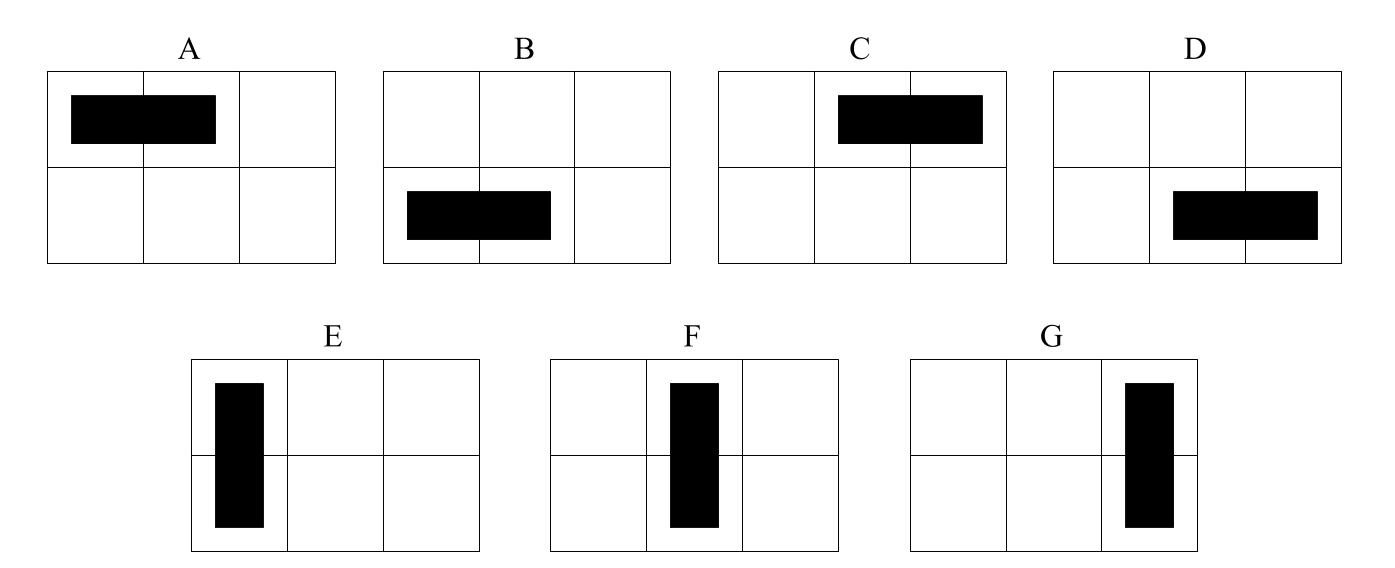
\includegraphics[width=1\textwidth]{figuras/posiciones-domino.png}
\end{figure}

\begin{figure}[ht]
\caption{Posibles posiciones de la ficha de dominó}
\label{fig:posiciones}
\centering
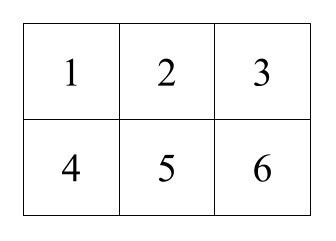
\includegraphics[width=0.4\textwidth]{figuras/posiciones.png}
\end{figure}

\begin{table}[ht]
\begin{center}
\caption[Matriz de pagos del juego con dominó]{Matriz de pagos del juego con dominó}
\label{table:pagos-domino}
\begin{tabular}{ c | c | c | c | c | c | c |}
  &  1 &  2 &  3 &  4 &  5 &  6 \\ \hline
A & -1 & -1 &  1 &  1 &  1 &  1 \\ \hline
B &  1 &  1 &  1 & -1 & -1 &  1 \\ \hline
C &  1 & -1 & -1 &  1 &  1 &  1 \\ \hline
D &  1 &  1 &  1 &  1 & -1 & -1 \\ \hline
E & -1 &  1 &  1 & -1 &  1 &  1 \\ \hline
F &  1 & -1 &  1 &  1 & -1 &  1 \\ \hline
G &  1 &  1 & -1 &  1 &  1 & -1 \\ \hline
\end{tabular}
\end{center}
\end{table}

El problema de programación lineal asociado es:
\begin{equation}
\begin{array}{r r r r r r r r r r r r r r r r r r}
max        &z& &   & &   & &   & &   & &   & &   & &   &      & \\
\text{s. a}
	& & &x_1&+&x_2&+&x_3&+&x_4&+&x_5&+&x_6&+&x_7& =    &1 \\
    &z&+&x_1&-&x_2&-&x_3&-&x_4&+&x_5&-&x_6&-&x_7& \leq &0 \\
    &z&+&x_1&-&x_2&+&x_3&-&x_4&-&x_5&+&x_6&-&x_7& \leq &0 \\
    &z&-&x_1&-&x_2&+&x_3&-&x_4&-&x_5&-&x_6&+&x_7& \leq &0 \\
    &z&-&x_1&+&x_2&-&x_3&-&x_4&+&x_5&-&x_6&-&x_7& \leq &0 \\
    &z&-&x_1&+&x_2&-&x_3&+&x_4&-&x_5&+&x_6&-&x_7& \leq &0 \\
    &z&-&x_1&-&x_2&-&x_3&+&x_4&-&x_5&-&x_6&+&x_7& \leq &0 \\
    & & &x_1,&&x_2,&&x_3,&&x_4,&&x_5,&&x_6,&&x_7,&\geq &0 \\
\end{array}
\end{equation}

Este problema no tiene solución única (lo que implica que el juego no tiene un equilibrio de Nash único), una solución viene dada por $(z^*, x^*_1, x^*_2, x^*_4, x^*_5, x^*_6, x^*_6, x^*_7) = (\frac{1}{3}, \frac{1}{3}, \frac{1}{3}, 0, 0, 0, 0, \frac{1}{3})$ y $(w^*, y^*_1, y^*_2, y^*_3,  y^*_4, y^*_5, y^*_6) = (\frac{1}{3}, \frac{1}{3}, 0, \frac{1}{3}, 0, \frac{1}{3}, 0)$, esta solución corresponde a la estrategia en la que el jugador $1$ elige las posiciones A, B y G con probabilidad $\frac{1}{3}$ cada una, y el jugador $2$ elige las posiciones $1$, $3$, y $5$ con probabilidad $\frac{1}{3}$ cada una.

\subsection{Coronel Blotto}
En este juego cada uno de los jugadores tiene $S$ soldados en total, y cada soldado puede ser asignado a uno de los $N$ campos de batalla. Cualquier número de soldados puede ser colocado en cualquier campo, incluyendo el cero. Un jugador obtiene un campo de batalla si asigna más soldados que su oponente en ese campo de batalla. El juego es ganado por el jugador que obtenga un mayor número de campos y su pago es igual a la diferencia entre el número de campos obtenidos por cada uno de los jugadores \cite{bib:introductionCFR}.

Formalmente el juego puede ser descrito de la siguiente manera. Cada jugador debe elegir $N$ números enteros, digamos $(a_1, a_2, ..., a_N)$ y $(b_1, b_2, ..., b_N)$, para el jugador $1$ y $2$ respectivamente, tales que $a_1 + a_2 + ... + a_N = S$ y $b_1 + b_2 + ... + b_N = S$, con $N < S$. Para estas distribuciones, la ganancia del jugador $1$ viene dada por:
\begin{alignat}{1}
|\{ 1 \leq i \leq N : a_i > b_i\}| - |\{ 1 \leq i \leq N : a_i < b_i\}|
\end{alignat}

\subsection{Kunh Poker}
Este juego fue descrito en la sección \ref{section:kuhn-poker}. A diferencia de los juegos anteriores, es un juego secuencial, por lo que su representación natural es en forma extensiva. Sin embargo, como se mostró en la sección \ref{section:normal-extensiva}, todo juego en forma extensiva puede ser representado en forma normal, por lo que se pueden aplicar los algoritmos a al forma normal correspondiente.

En este juego, el jugador $2$ tiene una ganancia esperada de $\frac{1}{18}$ por mano, como se prueba en \cite{bib:kuhn-poker}. Además, el primer jugador tiene infinitas estrategias óptimas, las cuales pueden ser representadas por la elección de un parámetro $\alpha \in [ 0, \frac{1}{3} ]$. Una vez elegido este parámetro, en la primera jugada del primer jugador, este apuesta con probabilidad $\alpha$ cuando su carta tenga el número $1$, apuesta con una probabilidad $3 \alpha$ cuando tiene el número $3$ y siempre pasa cuando tiene el número $2$. Si el primer jugador tiene un segundo turno, debe pasar siempre que tenga el número $1$, apostar cuando tiene el número $3$, y en el caso que tenga el número $2$ debe apostar con probabilidad $\alpha + \frac{1}{3}$.

El segundo jugador tiene una única estrategia mixta óptima: apostar siempre que tenga el número $3$. Cuando tenga el número $1$, pasar siempre que el primer jugador haya apostado y apostar con probabilidad $\frac{1}{3}$ en caso contrario. Cuando tenga el número $2$, debe pasar cuando el oponente haya pasado previamente y apostar con probabilidad $\frac{2}{3}$ en caso contrario. La figura \ref{fig:kunh-poker-estrategias} muestra el árbol con las distribuciones de probabilidad de las estrategias previamente descritas en cada uno de los nodos alcanzables en el juego.

\begin{figure}[ht]
\begin{center}
\caption{Equilibrio de Nash del juego de Kunh poker}
\label{fig:kunh-poker-estrategias}
\begin{tikzpicture}[
chance/.style={circle, draw=black, fill=gray, thick, minimum size = 6mm},
player1/.style={circle, draw=black, solid, thick, minimum size = 4mm},
player2/.style={circle, thick, minimum size=4mm},
terminal/.style={rectangle, draw=black, solid, fill=black, thick, minimum size=2mm},
level 1/.style={sibling distance=26mm, level distance=30mm},
level 2/.style={sibling distance=13mm, level distance=20mm},
level 3/.style={sibling distance=6.5mm, level distance=15mm},
]
\node[chance] [label=above:{Nodo de azar}] {} {
	child {node [player1] (P1) [label=above:{$(1, 2)$}]{}
		child { node [player2] [draw=red, fill=red] {} 
				child { node [terminal] [label=below:{$-1$}] {}
						edge from parent [dashed] node [left, draw=none] {\tiny{$1$}} {} }
				child { node [player1] (A) {} 
						child { node [terminal] [label=below:{$-1$}] {}
								edge from parent [dashed] {} }
						child { node [terminal] [label=below:{$-2$}] {} 
								edge from parent [solid, double] {} }
						edge from parent [solid, double] node [right, draw=none] {\tiny{$0$}}  {}
				}
				edge from parent [dashed] node [left, draw=none] {\tiny{$1-\alpha$}}  {}
		}
		child { node [player2] [draw=red] {} 
				child { node [terminal] [label=below:{$1$}] {}
						edge from parent [dashed] node [left, draw=none] {\tiny{$\frac{2}{3}$}} {} }
				child { node [terminal] [label=below:{$-2$}] {}
						edge from parent [solid, double] node [right, draw=none] {\tiny{$\frac{1}{3}$}} {} }
				edge from parent [solid, double] node [right, draw=none] {\tiny{$\alpha$}}{}
		}
	}
	child {node [player1] (P2) [label=above:{$(1, 3)$}]{}
		child { node [player2] [draw=blue, fill=blue] {} 
				child { node [terminal] [label=below:{$-1$}] {}
						edge from parent [dashed] node [left, draw=none] {\tiny{$0$}} {} }
				child { node [player1] (B) {} 
						child { node [terminal] [label=below:{$-1$}] {}
								edge from parent [dashed] node [left, draw=none] {\tiny{$1$}} {} }
						child { node [terminal] [label=below:{$-2$}] {}
								edge from parent [solid, double] node [right, draw=none] {\tiny{$0$}} {} }
						edge from parent [solid, double] node [right, draw=none] {\tiny{$1$}} {}
				}
				edge from parent [dashed] node [left, draw=none] {\tiny{$1-\alpha$}} {}
		}
		child { node [player2] [draw=blue] {} 
				child { node [terminal] [label=below:{$1$}] {}
						edge from parent [dashed] node [left, draw=none] {\tiny{$0$}} {} }
				child { node [terminal] [label=below:{$-2$}] {}
						edge from parent [solid, double] node [right, draw=none] {\tiny{$1$}} {} }
				edge from parent [solid, double] node [right, draw=none] {\tiny{$\alpha$}} {}
		}
	}
	child {node [player1] (P3) [label=135:{$(2, 1)$}]{}
		child { node [player2] [draw=green, fill=green] {} 
				child { node [terminal] [label=below:{$1$}] {}
						edge from parent [dashed] node [left, draw=none] {\tiny{$\frac{2}{3}$}} {} }
				child { node [player1] (C) {} 
						child { node [terminal] [label=below:{$-1$}] {}
								edge from parent [dashed] node [left, draw=none] {\tiny{$\frac{2}{3}-\alpha$}} {} }
						child { node [terminal] [label=below:{$2$}] {} 
                        		edge from parent [solid, double] node [right, draw=none] {\tiny{$\alpha+\frac{1}{3}$}} {} }
						edge from parent [solid, double] node [right, draw=none] {\tiny{$\frac{1}{3}$}} {}
				}
				edge from parent [dashed] node [left, draw=none] {\tiny{$1$}} {}
		}
		child { node [player2] [draw=green] {} 
				child { node [terminal] [label=below:{$1$}] {}
						edge from parent [dashed] {} }
				child { node [terminal] [label=below:{$2$}] {}
						edge from parent [solid, double] {} }
				edge from parent [solid, double] node [right, draw=none] {\tiny{$0$}} {}
		}
	}
	child {node [player1] (P4) [label=45:{$(2, 3)$}]{}
		child { node [player2] [draw=blue, fill=blue]{} 
				child { node [terminal] [label=below:{$-1$}] {}
						edge from parent [dashed] node [left, draw=none] {\tiny{$0$}} {} }
				child { node [player1] (D) {} 
						child { node [terminal] [label=below:{$-1$}] {}
								edge from parent [dashed] node [left, draw=none] {\tiny{$\frac{2}{3}-\alpha$}} {} {} }
						child { node [terminal] [label=below:{$-2$}] {}
								edge from parent [solid, double] {} node [right, draw=none] {\tiny{$\alpha+\frac{1}{3}$}} {} }
						edge from parent [solid, double] node [right, draw=none] {\tiny{$1$}} {}
				}
				edge from parent [dashed] node [left, draw=none] {\tiny{$1$}} {}
		}
		child { node [player2] [draw=blue] {} 
				child { node [terminal] [label=below:{$1$}] {}
						edge from parent [dashed] {} }
				child { node [terminal] [label=below:{$-2$}] {}
						edge from parent [solid, double] {} }
				edge from parent [solid, double] node [right, draw=none] {\tiny{$0$}} {}
		}
	}
	child {node [player1] (P5) [label=above:{$(3, 1)$}]{}
		child { node [player2] [draw=green, fill=green] {} 
				child { node [terminal] [label=below:{$1$}] {}
						edge from parent [dashed] node [left, draw=none] {\tiny{$\frac{2}{3}$}} {} }
				child { node [player1] (E) {} 
						child { node [terminal] [label=below:{$-1$}] {}
								edge from parent [dashed] node [left, draw=none] {\tiny{$0$}} {} }
						child { node [terminal] [label=below:{$2$}] {}
								edge from parent [solid, double] node [right,draw=none] {\tiny{$1$}} {} }
						edge from parent [solid, double] node [right, draw=none] {\tiny{$\frac{1}{3}$}} {}
				}
				edge from parent [dashed] node [left, draw=none] {\tiny{$1-3 \alpha$}} {}
		}
		child { node [player2] [draw=green] {} 
				child { node [terminal] [label=below:{$1$}] {}
						edge from parent [dashed] node [left, draw=none] {\tiny{$1$}} {} }
				child { node [terminal] [label=below:{$2$}] {}
						edge from parent [solid, double] node [right, draw=none] {\tiny{$0$}} {} }
				edge from parent [solid, double] node [right, draw=none] {\tiny{$3 \alpha$}} {}
		}
	}
	child {node [player1] (P6) [label=above:{$(3, 2)$}]{}
		child { node [player2]  [draw=red, fill=red] {} 
				child { node [terminal] [label=below:{$1$}] {}
						edge from parent [dashed] node [left, draw=none] {\tiny{$1$}} {} }
				child { node [player1] (F) {} 
						child { node [terminal] [label=below:{$-1$}] {}
								edge from parent [dashed] {}}
						child { node [terminal] [label=below:{$2$}] {}
								edge from parent [solid, double] {} }
						edge from parent [solid, double] node [right, draw=none] {\tiny{$0$}} {}
				}
				edge from parent [solid, double] node [left, draw=none] {\tiny{$1-3\alpha$}} {}
		}
		child { node [player2]  [draw=red] {} 
				child { node [terminal] [label=below:{$1$}] {}
						edge from parent [dashed] node [left, draw=none] {\tiny{$\frac{2}{3}$}} {} }
				child { node [terminal] [label=below:{$2$}] {}
						edge from parent [solid, double] node [right, draw=none] {\tiny{$\frac{1}{3}$}} {} }
				edge from parent [solid, double] node [right, draw=none] {\tiny{$3\alpha$}} {}
		}
	}
};
\end{tikzpicture}
\end{center}
\end{figure}
 % REORGANIZED: copied into regret-matching.tex
%\section{Detalles de Implementación}

En esta sección se describen los detalles relacionados a la implementación de los algoritmos utilizados para la parte experimental de la investigación. Los algoritmos fueron implementados en el lenguaje de programación C++, utilizando la librería estándar y una librería adicional llamada \textit{Eigen}, para factorizar matrices y resolver sistemas de ecuaciones.

\subsection{Regret Matching}
Se implementó una clase para encontrar un equilibrio de Nash mediante el algoritmo de \textit{Regret Matching}. En cada iteración la actualización de las estrategias depende de cada procedimiento según las fórmulas propuestas en la sección anterior.

\subsection{Juegos en forma extensiva}

Para representar el árbol en forma extensiva se creó la clase \textit{Nodo}, la cual tiene como atributos el jugador correspondiente, el conjunto de información, la distribución de probabilidad en caso que sea un nodo de azar y la ganancia del jugador $1$ en caso que sea un nodo terminal o apuntadores a sus hijos en caso que no lo sea.

El constructor de esta clase utiliza \textit{Depth First Search} para la lectura del árbol desde un archivo. El archivo de texto debe seguir el siguiente formato, una línea con tres valores enteros: el número del jugador ($p$), el conjunto de información ($I$) y el número de hijos del nodo ($N$). El nodo es de azar si el número del jugador es igual a cero, en este caso la línea debe tener $N$ números adicionales que sean una distribución de probabilidad sobre los hijos. Por otra parte, si el nodo es terminal ($N = 0$) entonces la línea debe tener un valor adicional que representa la utilidad para el jugador $1$. Una vez leído la información del nodo actual el constructor es llamado con cada uno de los hijos para construir cada uno de los subárboles.

\subsection{Forma normal a partir de la forma extensiva}
\label{subsec:FN-FE}

Para aplicar los algoritmos de \textit{Regret Matching} en juegos en formas extensiva es necesario hallar la forma normal correspondiente. Para esto se utiliza \textit{dfs} para determinar la cantidad de conjuntos de información de cada jugador y cuantas acciones diferentes tiene en cada uno, el árbol debe ser una instancia de la clase descrita anteriormente. Las estrategias puras son listadas usando \textit{backtracking} y para obtener el valor de pago se recorre el árbol mediante \textit{dfs}, pero sólo expandiendo los nodos que corresponden a la estrategia dada.

\subsection{Estrategia de comportamiento a partir estrategia mixta}
\label{subsec:EC-EM}
Una vez encontrado un equilibrio de Nash para la forma normal en un juego en forma extensiva originalmente, es deseable ser capaz de encontrar la estrategia de comportamiento respectiva. Debido a que más de un árbol pueden generar la misma matriz de pagos en forma normal, es necesario que tanto el árbol como la matriz de pagos sean proporcionados de forma explícita. Por otra parte, es necesario listar nuevamente todas las estrategias puras (de la misma forma que se listaron para encontrar la forma normal), para poder hacer la correspondencia entre cada estrategia pura del jugador $1$ y cada fila de la matriz, y cada estrategia pura del jugador $2$ y cada columna.

Para encontrar la distribución de probabilidad en cada conjunto de información se utiliza \textit{dfs} por cada estrategia mixta de cada jugador para encontrar, para cada conjunto de información $I$ y cada acción $a \in A(I)$, la probabilidad de alcanzar $I$ ($\pi(I)$) y la probabilidad de elegir la acción $a$ dado que $I$ es alcanzado. Luego, es utilizada la ecuación \ref{eq:mixta-a-comportamiento} para obtener cada una de las distribuciones de probabilidad. % REORGANIZED: copied into regret-matching.tex
%\section{Resultados Experimentales}

En esta sección se presenta un resumen de los resultados experimentales obtenidos utilizando el algoritmo \textit{Regret Matching} en los juegos descritos. Cada procedimiento fue probado $10$ veces por juego, finalizando cada corrida cuando se obtenía un regret máximo menor que $0.005$.

La tabla \ref{tab:resumen-resultados-RM} muestra un resumen de los resultados. En esta tabla se muestra, por cada juego, el tamaño de la matriz de pagos, el valor teórico del juego ($u_t$), el valor del juego utilizando la estrategia obtenida en la última corrida del algoritmo ($u_e$) y la explotabilidad ($\varepsilon_{\sigma}$). Las dos últimas métricas se presentan para cada uno de los procedimientos (A, B y C). En todos los casos se observa que la utilidad esperada para las estrategias obtenidas es cercana al valor del juego, además, se obtuvo una explotabilidad menor o igual que $0.011$, por lo que las estrategias obtenidas representan buenas aproximaciones al equilibrio de Nash en cada juego.

\begin{table}[htpb]
    \centering
    \begin{tabular}{l|r|r r r|r r r}
        &  & \multicolumn{3}{|c}{$u_e$} & \multicolumn{3}{|c}{$\varepsilon_{\sigma}$}  \\ \hline
        Juegos & $u_t$ & \multicolumn{1}{|c}{A} & \multicolumn{1}{c}{B} & \multicolumn{1}{c|}{C}
          & \multicolumn{1}{|c}{A} & \multicolumn{1}{c}{B} & \multicolumn{1}{c}{C} \\ \hline
        Matching Pennies
            & $0$ & $0$ & $0$ & $0$ & $0.006$ & $0.006$ & $0.008$ \\
        Piedra, Papel o Tijeras
            & $0$ & $-0.000012$ & $0.000004$ & $0.000022$ & $0.006$ & $0.01$ & $0.009$ \\
        Ficha vs. Dominó
            & $\frac{1}{3}$ & $0.333$ & $0.334$ & $0.334$ & $0.01$ & $0.007$ & $0.004$ \\
        Coronel Blotto
            & $0$ & $0.000219$ & $-0.000502$ & $0.000024$ & $0.01$ & $0.011$ & $0.009$ \\
        \hline
    \end{tabular}
    \caption{Resumen de los resultados y evaluación de las estrategias obtenidas usando el algoritmo de Regret Matching en juegos en forma normal}
    \label{tab:resumen-resultados-RM}
\end{table}

Para evaluar la convergencia se midió el tiempo necesario para alcanzar el regret desea y el número de iteraciones, en la Tabla \ref{tab:resumen-regret-tiempo-RM} se presenta el tiempo ($T$), el número de iteraciones ($I$) y el tiempo por iteración ($T/I$) obtenido para cada uno de los juegos para cada procedimiento. Estos resultados son el promedio de las $10$ corridas realizadas por juego y procedimiento. Además, se crearon gráficas del regret por iteración para observar como disminuye a medida que corre el algoritmo, la  Figura  \ref{fig:regret-blotto} muestra las gráficas para el juego Coronel Blotto y los $3$ procedimientos. Estas gráficas son mostradadas con una escala logarítmica en el eje $x$ para apreciar mejor los resultados. En el Apéndice A se muestran las tablas detalladas con los resultados en cada una de las corridas y las gráficas de cada juego con los $3$ procedimientos.

\begin{figure}[htpb!]
    \caption{Gráficas del regret con respecto al número de iteraciones del juego Coronel Blotto}
    \label{fig:regret-blotto}
    \centering
    \includegraphics[width=0.58\textwidth]{graficas/coronel-blotto/procedimiento-A.png}
    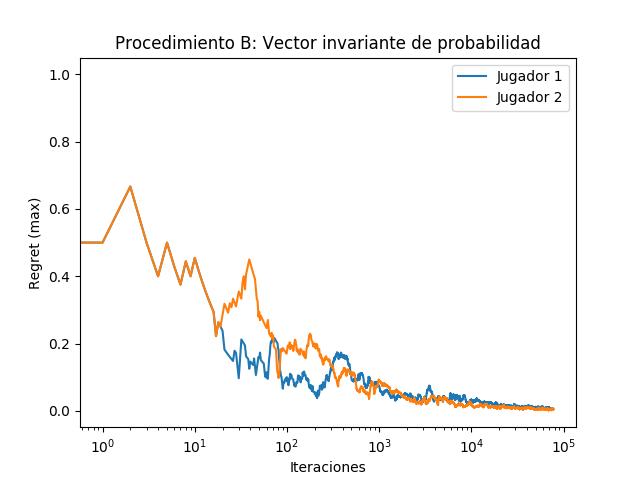
\includegraphics[width=0.58\textwidth]{graficas/coronel-blotto/procedimiento-B.png}
    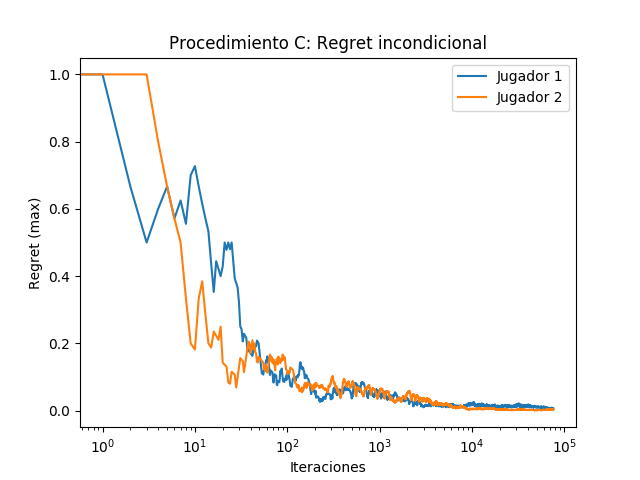
\includegraphics[width=0.58\textwidth]{graficas/coronel-blotto/procedimiento-C.png}
\end{figure}

\begin{table}[htpb]
    \centering
    \begin{tabular}{l | c |r r r}
        Juegos & Proc. & $T$ & $I$ & $T/I$ \\ \hline
        \multirow{3}{*}{Matching Pennies}
            & A & $10.276$ & $3892550.4$ & $2.64 {\times} 10^{-06}$ \\
            & B &  $0.777$ &   $25616.6$ & $3.03 {\times} 10^{-05}$ \\
            & C &  $0.042$ &   $16260.5$ & $2.58 {\times} 10^{-06}$ \\ \hline
        \multirow{3}{*}{Piedra, Papel o Tijeras}
            & A & $12.198$ & $4519054.1$ & $2.70 {\times} 10^{-06}$ \\
            & B &  $0.345$ &    $6601.3$ & $5.23 {\times} 10^{-05}$ \\
            & C &  $0.049$ &   $19321.1$ & $2.54 {\times} 10^{-06}$ \\ \hline
        \multirow{3}{*}{Ficha vs. Dominó}
            & A & $319.179$ & $108319272.4$ & $2.95 {\times} 10^{-06}$ \\
            & B &  $11.275$ &     $75250.2$ & $1.50 {\times} 10^{-04}$ \\
            & C &   $0.237$ &     $84318.5$ & $2.81 {\times} 10^{-06}$ \\ \hline
        \multirow{3}{*}{Coronel Blotto}
            & A & $875.533$ & $190222305.3$ & $4.60 {\times} 10^{-06}$ \\
            & B &  $79.358$ &     $66378.4$ & $1.20 {\times} 10^{-03}$ \\
            & C &   $0.166$ &     $48613.5$ & $3.41 {\times} 10^{-06}$ \\ \hline
    \end{tabular}
    \caption{Resumen de los resultados y evaluación de las estrategias obtenidas usando el algoritmo de Regret Matching en juegos en forma normal}
    \label{tab:resumen-regret-tiempo-RM}
\end{table}

A continuación se se analiza el desempeño de los procedimientos, comparándolos entre sí, observando la rapidez de convergencia de cada uno de ellos.

\subsection{Complejidad de cada iteración}

Los procedimientos cambian en la forma en que se elige la siguiente estrategia en cada iteración. En los procedimientos A y B se utiliza un regret condicional, en el que se mide el \textit{arrepentimiento} de cambiar una estrategia por otra en específica. Esta métrica se debe mantener a lo largo de todas las iteraciones, por lo que cada iteración necesita memoria adicional de complejidad $\mathcal{O}(N^2 + M^2)$, donde $N$ y $M$ es el número de acciones posibles para el jugador $1$ y $2$, respectivamente. En el procedimiento C se utiliza únicamente el regret incondicional, por lo que la cantidad de memoria adicional es del orden $\mathcal{O}(N + M)$.

Con respecto a la complejidad de tiempo se tiene que los procedimientos de regret condicional e incondicional (A y C), son lineales al número de acciones. Sin embargo, en el procedimiento B es necesario resolver un sistema de ecuaciones lineales para elegir cada estrategia nueva, del tamaño del número de acciones del jugador respectivo, obteniendo que la complejidad total es $\mathcal{O}(N^3 + M^3)$. La Tabla \ref{tab:complejidades-iteraciones} muestra un resumen de la complejidad es tiempo y memoria adicional.

\begin{table}[ht]
    \centering
    \begin{tabular}{c|c|c}
         Procedimiento & Memoria & Tiempo  \\ \hline
         A & $\mathcal{O}(N^2 + M^2)$ & $\mathcal{O}(N + M)$ \\ 
         B & $\mathcal{O}(N^2 + M^2)$ & $\mathcal{O}(N^3 + M^3)$ \\
         C & $\mathcal{O}(N + M)$     & $\mathcal{O}(N + M)$ \\ \hline
    \end{tabular}
    \caption{Complejidad por iteración de cada uno de los procedimientos}
    \label{tab:complejidades-iteraciones}
\end{table}

Por lo anterior, se observa que la velocidad de las iteraciones del procedimiento que calcula el vector invariante de probabilidad es más lenta en todos los casos, estando uno o dos órdenes de magnitud por encima, según el tamaño de la matriz. Por lo que, si la matriz es sumamente grande, el segundo método sería el menos adecuado.

\subsection{Número de iteraciones}

En la Tabla \ref{tab:resumen-regret-tiempo-RM} se puede observar un resumen de las iteraciones promedio de los tres procedimientos en cada uno de los juegos. Se nota que el procedimiento A, regret incondicional es el que necesita muchas más iteraciones para converger. Con respecto a los procedimientos B y C, se observa que en algunos casos el promedio en el procedimiento B fue menor y en otros el promedio del procedimiento C. También es importante destacar que en el juego de piedra, papel o tijera se tienen varios casos donde se obtiene la convergencia en menos de $10$ iteraciones (ver apéndice A), esos son casos donde se obtiene el equilibrio de Nash de forma exacta en pocas iteraciones.

\subsection{Tiempo transcurrido}

Observando el tiempo promedio de los procedimientos en la tabla \ref{tab:resumen-regret-tiempo-RM}, se nota que el procedimiento A es el que emplea más tiempo en todos los casos, esto ocurre porque necesita muchas más iteraciones que los otros dos procedimientos. Por otra parte el procedimiento C es también más rápido que el procedimiento B, ya que la complejidad en cada iteración para resolver el sistema de ecuaciones enlentece el tiempo total necesario, incluso, si la matriz es muy grande este procedimiento podría ser más lento que el procedimiento A y no sería factible.

Aunque el procedimiento donde se aplica regret matching al regret incondicional (procedimiento C), es el más sencillo de implementar y el más rápido en converger, este procedimiento tiene una desventaja con respecto a los otros dos. Al utilizar el regret condicional, los dos primeros procedimientos garantizan que el regret condicional tiende a cero para cualquier par de estrategias de cada jugador y por lo tanto, conducen siempre a un equilibrio correlacionado. El tercer procedimiento sólo minimiza el regret incondicional y por lo tanto, si el juego es de más de dos jugadores o no es de suma cero, entonces ya no es de utilidad para hallar alguna solución del juego.

 % REORGANIZED: copied into regret-matching.tex
%\chapter{Conterfactual Regret Minimization}
%\section{Monte Carlo Conterfactual Regret Minimization}

En la sección \ref{section:cfr} se explicó el algoritmo de CFR, utilizado para resolver juegos en forma extensiva. Sin embargo, en la versión presentada es necesario recorrer el árbol completo en cada iteración, esta versión suele conocerse como \textit{vanilla} CFR. En \cite{bib:montecarlo-cfr} se describe una familia general de algoritmos CFR (basados en muestreo) denominada \textbf{Monte Carlo Conterfactual Regret Minimization} (MCCRF), para evitar recorrer el árbol completo en cada iteración.

La idea general es restringir los estados terminales alcanzados en cada iteración, pero manteniendo el mismo valor esperado para la utilidad contrafactual. Dada la definición \ref{def:informacion-incompleta}, sea $\mathcal{Q} = \{Q_1, Q_2, ..., Q_r\}$, un conjunto de subconjuntos de $Z$ tal que su unión sea igual a $Z$. Cada uno de estos conjuntos será llamado un bloque. Sea $q_j > 0$ la probabilidad de considerar el bloque $Q_j$ para la iteración actual (donde $\sum_{j = 1}^r {q_j} = 1$). 
Sea $q(z) = \sum_{j | j \in Q_i}$, es decir, $q(z)$ es la probabilidad de considerar $z$ en la iteración actual. La utilidad contrafactual muestreada, cuando se actualiza el bloque $j$ es:

\begin{alignat}{1}
\tilde{u}_i(\sigma, I | j) = \sum_{h \in I, z \in Q_j} \frac{\pi^{\sigma_{-i}}(h) \pi^{\sigma}(h, z) u_i(z)}{q(z) \pi^{\sigma_{-i}}(I)}
\end{alignat}

\begin{lemma}
$E_{j \sim q_j} [\tilde{u}_i(\sigma, I | j)] = u_i(\sigma, I)$
\end{lemma}

\begin{proof}
\begin{alignat}{2}
    E_{j \sim q_j}[\tilde{u}_i(\sigma, I | j)] & = \sum_{j} {q_j u_i(\sigma, I)} \\
    & = \sum_{j} { q_j \frac{\sum_{h \in I, z \in Q_j} \pi^{\sigma_{-i}}(h) \pi^{\sigma}(h, z) u_i(z)}{q(z) \pi^{\sigma_{-i}}(I)}} \\ \label{eq:def-esperanza}
    & = \sum_{j} \sum_{ \substack{h \in I \\ z \in Q_j}} \frac{q_j \pi^{\sigma_{-i}}(h) \pi^{\sigma}(h, z) u_i(z)}{ q(z) \pi^{\sigma_{-i}}(I)} \\ \label{eq:reorder-sum-1}
    & = \sum_{ \substack{h \in I \\ z \in Z} } \sum_{j | z \in Q_j} \frac{q_j \pi^{\sigma_{-i}}(h) \pi^{\sigma}(h, z) u_i(z)}{ q(z) \pi^{\sigma_{-i}}(I)} \\ \label{eq:reorder-sum-2}
    & = \sum_{ \substack{h \in I \\ z \in Z} } \left(\frac{\sum_{j | z \in Q_j} q_j }{q(z)}\right) \frac{\pi^{\sigma_{-i}}(h) \pi^{\sigma}(h, z) u_i(z)}{\pi^{\sigma_{-i}}(I)} \\
    & = \sum_{ \substack{h \in I \\ z \in Z} } \frac{\pi^{\sigma_{-i}}(h) \pi^{\sigma}(h, z) u_i(z)}{\pi^{\sigma_{-i}}(I)}  = u_i(\sigma, I) \label{eq:lemma-final-eq}
\end{alignat}

La ecuación \ref{eq:def-esperanza} se obtiene de la definición de $\tilde{u}_i(\sigma, I | j)$. \ref{eq:reorder-sum-1} y \ref{eq:reorder-sum-2} se obtienen al reordenar las sumatorias y considerando que la unión de los bloques generan a $Z$. La ecuación \ref{eq:lemma-final-eq}
\end{proof}

Si se elige $\mathcal{Q} = {Z}$, es decir un único bloque con todas las historias terminales y $q_1 = 1$, la utilidad contrafactual es igual a la utilidad contrafactual muestreada y se obtiene el algoritmo \textit{vanilla} CFR. Si se eligen los bloques para incluir todas las historias terminales con la misma secuencia de acciones en los nodos de azar se obtiene el \textit{chance-sampled} CFR, siendo esta última versión la utilizada para estudiar los juegos presentados en este trabajo de grado. Se implementa el algoritmo como es detallado en \cite{bib:introductionCFR} que se presenta en el \textit{\textbf{apéndice X}}. % REORGANIZED: copied into ch6-CFR.tex
%\section{Evaluación de las estrategias y explotabilidad}

Para evaluar la convergencia de los algoritmos y la estrategia obtenida se utilizaron las métricas de \textit{regret} y explotabilidad, respectivamente.

La explotabilidad se obtiene al calcular la mejor respuesta de la estrategia de cada jugador y sumar los resultados, como se explicó en la sección \textit{\textbf{Explicar explotabilidad en el capítulo 2}}. Sin embargo, la diferencia es que en los juegos de forma extensiva no se pueden listar todas las estrategias fácilmente como en los juegos en forma normal, ya que esta tarea es exponencial en el tamaño del árbol.

Para calcular la explotabilidad en estos juegos se utilizó el algoritmo propuesto en \cite{bib:thesis-marc-lanctot}, denominado \textit{Generalized Expectimax Best Response} (GEBR), descrito en el apéndice \textit{\textbf{X}}. La complejidad de este algoritmo es $\mathcal{O}(ND)$ donde $N$ es el número de nodos del árbol y $D$ es la profundidad del árbol. Note que el algoritmo tiene una alta complejidad, por lo que se usará únicamente para calcular la explotabilidad de la estrategia final. % REORGANIZED: copied into ch6-CFR.tex
%\section{Detalles de implementación}
Los algoritmos y la representación de los juegos fueron implementados en el lenguaje de programación C++. Para la representación de los juegos se utilizó una clase abstracta llamada \textit{Game}, que recibe como template los tipos para el estado, las acciones, las propiedades, los conjunto de información y el Hash del juego específico.

Esta clase contiene las funciones virtuales necesarias para recorrer el árbol del juego de forma \textbf{implícita}, tales como: \textit{actions}, que retornan las acciones del juegos en el estado actual, \textit{update\_state}, que actualiza el estado del juego dada una acción a realizar, \textit{terminal\_state} que indica si un estado es terminal o no, \textit{utiliy} que retorna la utilidad en un estado terminal, entre otras. Los algoritmos CFR y GEBR utilizan esta clase abstracta en su implementación.

Para cada tipo de juego, se creó una clase derivada de la clase \textit{Game}, donde se implementaron las funciones según las reglas de cada juego. De esta forma se puede utilizar la misma implementación de los algoritmos para todos los juegos.

Cabe destacar que todos los juegos fueron representados mediantes árboles con la raíz como único nodo de azar. Algunos juegos tienen esta representación de forma natural, por ejemplo, el Kuhn Poker, ya que las cartas se reparten al inicio y luego se juega acorde a esa distribución, sin volver a introducir ninguna jugada aleatoria. Otros juegos pueden tener nodos de azar distintos a la raíz, sin embargo siempre es posible transformarlos a un árbol que represente el mismo juego donde todos los nodos de azar son condensados en la raíz y cada hijo de la raíz representa una elección por cada uno de los nodos de azar del árbol original. En esta representación se asume que todas las decisiones aleatorias se toman al inicio del juego.

La clase \textit{Game} y todos los algoritmos se implementados suponiendo la raíz como único nodo de azar del juego. % REORGANIZED: copied into ch6-CFR.tex
%\section{Descripción de los juegos}
\label{section-description-juegos-forma-extensiva}

Para probar los algoritmos se implementaron tres tipos de juegos diferentes: \textit{One Card Poker} (OCP), \textit{Dudo}, un juego de dados, y una versión del juego de dominó para $2$ personas. La descripción detallada de las reglas de los juegos se describen en esta sección.

\subsection{One-Card Poker}
One-Card Poker, abreviado OCP(N), es la versión generalizada del juego Kuhn Póker, explicado en la sección \ref{section:kuhn-poker}. En este juego, cada jugador recibe una carta de un mazo de $N$ cartas, y luego pueden apostar o retirarse según las mismas reglas del Kuhn Póker. Note que OCP(3) es equivalente al Kuhn Poker. El árbol de este juego tiene $9N(N-1)+1$ nodos (incluyendo el nodo inicial, que es el nodo de azar) y hay $4N$ conjuntos de información entre ambos jugadores. 

\subsection{Dudo}
Dudo, también conocido como \textit{Bluff}, \textit{Liar's Dice} o Perudo, es un juego de dados y apuestas. Usualmente se juega entre $2$ y $6$ jugadores. Los jugadores se ubican en forma circular y cada uno de ellos tiene un número de dados. De forma simultánea, todos lanzan sus dados, cada jugador puede ver el resultado de sus propios dados, pero no puede ver el resultado de los dados de los otros jugadores. Una vez hecho esto, los jugadores empiezan a apostar sobre el número de veces que apareció una cara en específico en todos los dados que hay en la mesa.

Una apuesta consiste en decir $2$ números $(x, y)$, esto indica que el jugador apuesta que hay, al menos, $x$ dados cuyo resultado fue el número $y$. El primer jugador (que se elige previamente mediante el lanzamiento de $1$ dado o de alguna otra forma), realiza la primera apuesta y, en sentido horario, cada jugador puede hacer una apuesta más alta o decir \say{dudo} y retar al jugador anterior. Una apuesta es más alta que otra si el número de dados que se anuncian en la apuesta ($x$) es mayor, o si el número de dados es igual, pero la cara apostada ($y$) es mayor. Por ejemplo $(3, 1)$ es mayor que $(2, 5)$, y ambas apuestas son mayores que $(2, 3)$.

Por otra parte, si un jugador reta al jugador previo, se descubren todos los dados de todos los jugadores. Si la cantidad de dados con la cara $y$ es mayor o igual a $x$, donde $(x, y)$ fue la apuesta realizada por el jugador, el jugador que hizo el reto pierde un dado. En caso contrario, el jugador que hizo la apuesta pierde un dado. Luego, todos los jugadores lanzan sus dados nuevamente y una nueva ronda de apuestas empieza por el jugador que perdió la ronda anterior. Un jugador pierde cuando se queda sin dados, el ganador es el último jugador con al menos un dado restante. La figura \ref{fig:dudo} muestra una foto del juego, de \textit{Perudo}, una versión comercial de este juego, que está diseñada para $6$ jugadores, donde cada jugador empieza con $5$ dados. En la figura se observan los vasos que se utilizan para lanzar los dados y evitar que cada jugador vea los dados de los demás.

\begin{figure}[htb]
\caption[Juego Dudo]{Juego Dudo. Los vasos se utilizan para lanzar los dados y evitar que los oponentes vean el resultado}
\label{fig:dudo}
\centering
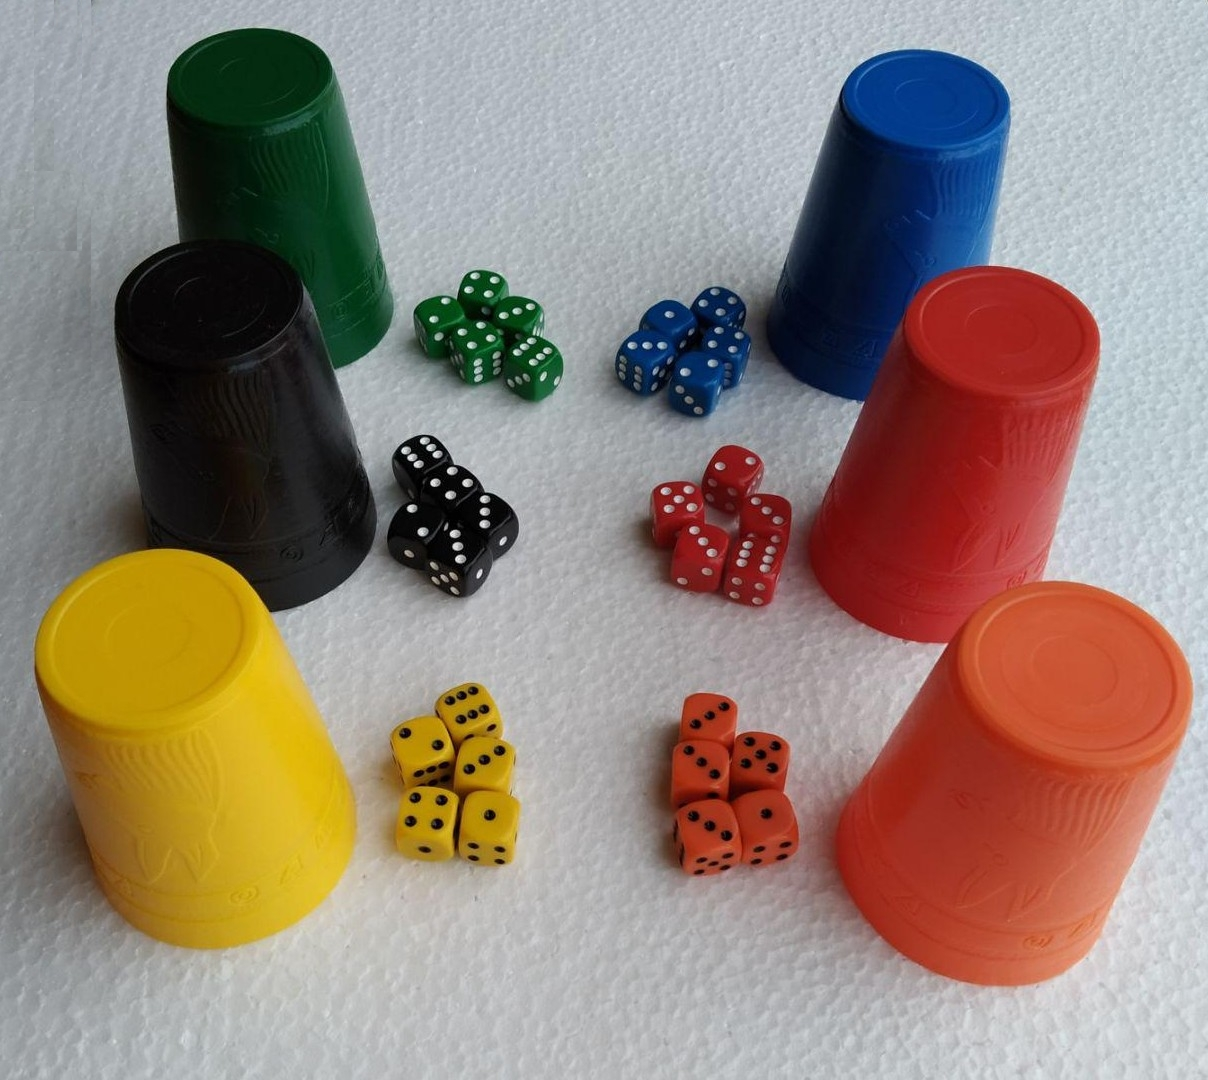
\includegraphics[width=0.6\textwidth]{figuras/dudo.jpg}
\end{figure}

En este trabajo de grado consideraremos este juego para $2$ jugadores únicamente. Dudo$(K, D_1, D_2)$ hará referencia a una única ronda de apuestas de $2$ jugadores, donde el primer jugador tiene $D_1$ dados, el segundo jugador tiene $D_2$ dados y cada dado tiene $K$ caras. El juego completo consiste en múltiples rondas, donde $D_1$ o $D_2$ disminuye en una unidad al finalizar cada ronda. Cuando uno de los jugadores pierde todos los dados obtiene una utilidad de $-1$, mientras que su oponente obtiene una utilidad de $1$. En este juego cada ronda se considerará un subjuego y se representará con un árbol independiente, donde los valores esperados para los juegos Dudo$(K, D_1 - 1, D_2)$ y Dudo$(K, D_1, D_2 - 1)$ se precalculan y se utilizan como utilidad para las hojas del árbol Dudo$(K, D_1, D_2)$. Note que, en el juego estándar, $K$ siempre tiene un valor de $6$.

Cuando el jugador $i$ lanza $D_i$ dados hay $\binom{D_i+K-1}{K-1}$ resultados posibles diferentes, ya que cada resultado puede ser representado con una tupla $(a_1, a_2, ..., a_k)$, donde $a_j$ representa el número de dados con la cara $j$, por lo que $\sum_j^K = D_i$ y $a_j \geq 0$. Por otra parte cada secuencia de apuestas puede ser representada por una secuencia binaria de longitud $K(D_1 + D_2)$, donde el $i$-ésimo bit es $1$ si la $i$-ésima secuancia más fuerte fue dicha durante la ronda y $0$ en caso contrario. Por ejemplo, si $D_1 = D_2 = 1$, las apuestas $(1, 1)-(1, 3)-(1, 6)-(2, 4)-(2, 5)-(1, 6)$ se representa con la secuencia binaria $101001000110$, por lo que hay $2^{K(D_1 + D_2)}$ secuencias diferentes. Cada secuencia pertenece a un jugador en específico, por lo que si $D_1 = D_2$, el número de conjuntos de información  es igual a  $\binom{D_i+K-1}{K-1}2^{K(D_1 + D_2)}$.

Para contar el número total de nodos, se puede considerar el lanzamiento de los dados de forma independiente, pues las secuencias posibles de apuestas no dependen del resultado de los dados. Por lo expuesto anteriormente el número posible de apuestas es igual a $2^{K(D_1+D_2)}$, pero después de cada secuencia siempre se puede decir \say{dudo}, salvo para la secuencia vacía. Luego el número total de nodos (incluyendo nodos terminales y no terminales) es igual a $\binom{D_1+K-1}{K-1}\binom{D_1+K-1}{K-1}(2^{K(D_1+D_2)+1}-1)+1$.

\subsection{Domino}
En este trabajo se utilizó una versión de este juego para $2$ jugadores. Al inicio del juego cada jugador toma una cantidad específica de piezas de forma aleatoria, las piezas restantes se dejan sin descubrir para ser usadas en turnos posteriores. Como en el juego tradicional de dominó, los jugadores juegan por turnos alternados (el primero jugador se elige de forma arbitraria), cada uno debe colocar una ficha válida acorde a las reglas \textit{estándares} en Venezuela del juego (ver apéndice \textit{\textbf{X}}). Si un jugador no puede colocar una ficha toma una ficha de las que no están descubiertas (si todavía hay disponibles), el jugador verifica si puede colocar la ficha tomada y en caso contrario pasa el turno y juega el oponente.

El juego termina cuando alguno de los jugadores usa todas las piezas o cuando ambos jugadores no pueden jugar ni tomar piezas nuevas, en este último caso se dice que el juego está bloqueado. El ganador es el jugador que se queda sin piezas o, en caso de bloqueo, el jugador que acumule menos puntos en todas las piezas que quedaron en su mano. La utilidad obtenida es el número de puntos que el jugador perdedor acumuló en las piezas que quedaron en su mano (con signo positivo para el jugador ganador y signo negativo para el perdedor). Cabe destacar que sólo se puede tomar una pieza o pasar, si no se puede realizar una jugada con la mano actual.

Usualmente se utilizan $28$ piezas, donde las piezas pueden tener entre $0$ y $6$ puntos en cada extremo, y cada jugador recibe $7$ piezas al inicio del juego. En este trabajo se parametriza el número máximo de puntos que puede tener una ficha, así como la cantidad de piezas repartidas inicialmente. De esta forma se hará referencia a Domino$(M, N)$ an un juego donde las piezas tienen entre $0$ y $M$ puntos (con un total de $M(M+1)/2$ piezas) y cada jugador recibe $N$ piezas al inicio del juego.

En este juego no es fácil calcular el tamaño del árbol y el número de conjuntos de información, principalmente porque las acciones posibles en un estados dependen tanto de la mano del jugador, como de las piezas en la mesa. En el Kuhn Póker simpre hay $2$ acciones posibles ${pasar, apostar}$ y en el Dudo las acciones disponibles dependen únicamente de la última apuesta y no dependen de los dados que tengan los jugadores. Así que se decidió estimar estos parámetros recorriendo el árbol del juego mediante DFS. La tabla \ref{tab:tree-domino}, muestra el número de nodos del árbol y el número de conjuntos de información por cada juego de dominó que se presenta.

\begin{table}[ht]
    \centering
    \begin{tabular}{c|r|r}
        & Conjutos de Información & Nodos \\ \hline
       Domino$(1, 1)$ & $3$ & $13$ \\
       Domino$(2, 2)$ & $441$   & $7321$ \\
       Domino$(3, 2)$ & $844437$   & $46534657$ \\
       Domino$(3, 3)$ & $1082290$   & $246760993$ \\ 
       Domino$(3, 4)$ & $902218$   & $1547645185$ \\ \hline
    \end{tabular}
    \caption{Número de nodos y conjuntos de Información en diferentes juegos de Dominó}
    \label{tab:tree-domino}
\end{table}


 % REORGANIZED: copied into ch6-CFR.tex
%\subsection{Resultados experimentales}

Se crearon varias instancias de los $3$ juegos explicados en la sección \ref{section-description-juegos-forma-extensiva} con diferentes parámetros. Para cada instancia se utilizó el algoritmo de CFR y se iteró sobre el árbol durante $10$ (\textit{\textbf{número tentativo}}) horas (se excluye el tiempo que se calcula el regret ya que no forma parte del algoritmo y esto se hace únicamente para obtener las gráficas). Una vez terminado el tiempo asignado se calcula la mejor respuesta para cada jugador y la explotabilidad. Una instancia de un juego se considerará resuelta si la explotabilidad de la estrategia obtenida es menor que el $1\%$ de la mínima unidad de utilidad posible según cada juego.

La tabla \ref{tab:resultados-CFR} resume los resultados, donde $N$ representa el número de nodos del árbol $I$ el número de conjuntos de información, $u_{\sigma}$ el valor del juego usando la estrategia obtenida y $\varepsilon_{\sigma}$ la explotabilidad. También se agrega el número de iteraciones y la última columna indica si el juego fue resuelto o no, según lo establecido en el párrafo anterior.

\begin{table}[ht]
    \centering
    \begin{tabular}{l|r|r|r|r|r|c}
        Juego & $N$ & $I$ & Iteraciones & $u$ & $\varepsilon$ & Resuelto \\ \hline
        OCP$(3)$    &        $55$ &    $12$ & & & & \cmark \\
        OCP$(12)$   &      $1189$ &    $48$ & & & & \cmark \\
        OCP$(50)$   &     $22051$ &   $200$ & & & & \cmark \\
        OCP$(200)$  &    $358201$ &   $800$ & & & & \cmark \\
        OCP$(1000)$ &   $8991001$ &  $4000$ & & & & \cmark \\
        OCP$(4000)$ & $143964001$ & $16000$ & & & & \cmark \\
        \hline
        Dudo$(3, 1, 1)$ &      $1144$ &      $192$ & & & & \cmark \\
        Dudo$(3, 2, 1)$ &     $18415$ &     $2304$ & & & & \cmark \\
        Dudo$(3, 1, 2)$ &     $18415$ &     $2304$ & & & & \cmark \\
        Dudo$(3, 2, 2)$ &    $294877$ &    $24576$ & & & & \cmark \\
        Dudo$(4, 1, 1)$ &      $8177$ &     $1024$ & & & & \cmark \\
        Dudo$(4, 2, 1)$ &    $327641$ &    $28672$ & & & & \cmark \\
        Dudo$(4, 1, 2)$ &    $327641$ &    $28672$ & & & & \cmark \\
        Dudo$(4, 2, 2)$ &  $13107101$ &   $655360$ & & & & \xmark \\
        Dudo$(5, 1, 1)$ &     $51176$ &     $5120$ & & & & \cmark \\
        Dudo$(5, 2, 1)$ &   $4915126$ &   $327680$ & & & & \cmark \\
        Dudo$(5, 1, 2)$ &   $4915126$ &   $327680$ & & & & \cmark \\
        Dudo$(5, 2, 2)$ & $471858976$ & $15728640$ & & & & \xmark \\
        Dudo$(6, 1, 1)$ &    $294877$ &    $24576$ & & & & \cmark \\
        Dudo$(6, 2, 1)$ &  $66060163$ &  $3538944$ & & & & \cmark \\
        Dudo$(6, 1, 2)$ &  $66060163$ &  $3538944$ & & & & \cmark \\
        Dudo$(6, 2, 2)$ &  $14797504071$ &  $352321536$ & & & & \xmark \\
        \hline
        Domino$(2, 2)$ &     $441$ &       $7321$ & & & & \cmark \\
        Domino$(3, 2)$ &  $844437$ &   $46534657$ & & & & \cmark \\
        Domino$(3, 3)$ & $1082290$ &  $246760993$ & & & & \cmark \\
        Domino$(3, 4)$ &  $902218$ & $1547645185$ & & & & \cmark \\
        Domino$(4, 2)$ & & & & & & \xmark \\
        \hline
    \end{tabular}
    \caption{Resultados del algortimo CFR en los diferentes juegos}
    \label{tab:resultados-CFR}
\end{table}

La gráfica \textit{\textbf{Mostrar una o dos gráficas interesantes y decir algo al respecto}}. En el apéndice \textit{\textbf{X}} se pueden observar todas las gráficas del regret con respecto al número de iteraciones, se nota que el regret tiende a $0$ en todos los casos (\textit{\textbf{Agregar algún otro detalle interesante que se vea en las gráficas}}) % REORGANIZED: copied into ch6-CFR.tex
\chapter*{Conclusiones}

Sugerencias y revisiones de esta clase enviarlos a los correos \texttt{ccontreras@usb.ve} y \texttt{asajo@usb.ve}.
\nocite{*}
\bibliography{referencias}
\appendix
\chapter{Resultados Experimentales. Regret Matching en Juegos en Forma Normal}

Para cada uno de los juegos se muestra una tabla con la estrategia obtenida en la última corrida de cada uno de los procedimientos y, en caso de conocerse, el equilibrio de Nash. Para cada estrategia se muestra el \textit{peor caso} de cada jugador. Es decir, el peor caso para el jugador $i$ cuando utiliza la estrategia $\sigma_{i}$ es $u_i(\sigma_i, \sigma^*_{-i})$, donde $\sigma^*_{-i}$ es mejor respuesta a $\sigma_i$.

Por otra parte, para cada juego se presenta una tabla que indica el tiempo de cada corrida ($T$), el número de iteraciones para alcanzar la cota deseada ($I$) y el tiempo promedio de cada iteración en cada una de las corridas ($T/I$), así como el promedio del tiempo y del número de iteraciones para cada procedimiento. Además, también se muestran las gráficas del \textit{regret} por iteraciones, para observar su convergencia. Estas gráficas son mostradadas con una escala logarítmica en el eje $x$ para apreciar mejor los resultados.

\newcommand{\graphicsRM}[2]{
\begin{figure}[htpb!]
    \caption{Gráficas del regret con respecto al número de iteraciones del juego #1}
    \label{fig:regret-#2}
    \centering
    \includegraphics[width=0.497\textwidth]{graficas/#2/procedimiento-A.png}
    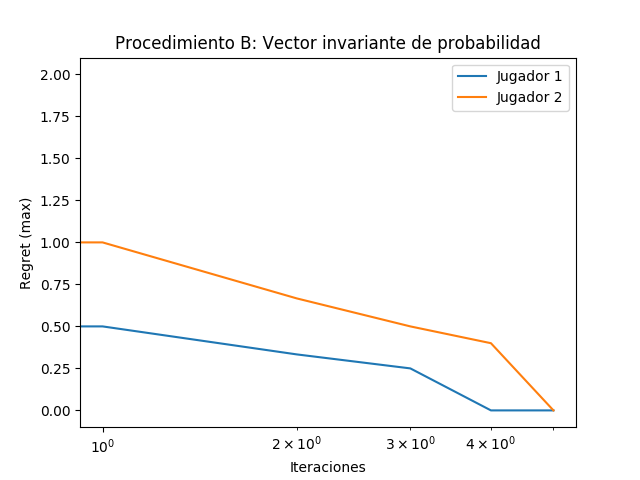
\includegraphics[width=0.497\textwidth]{graficas/#2/procedimiento-B.png}
    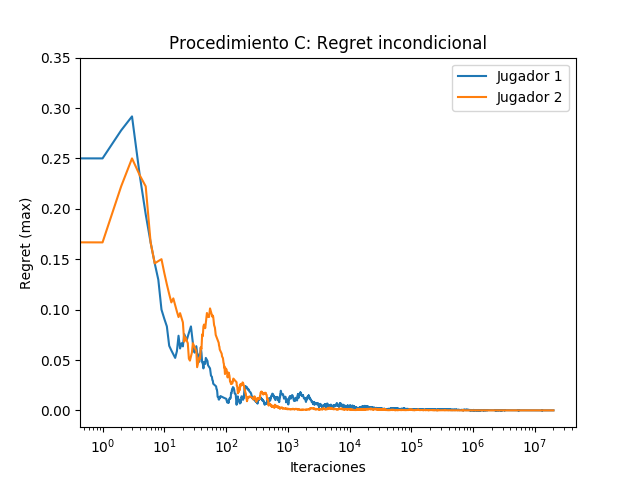
\includegraphics[width=0.497\textwidth]{graficas/#2/procedimiento-C.png}
\end{figure}
}

\section{Matching Pennies}

En este juego, si un jugador elige cada acción con una probabilidad de $0.5$, entonces su ganancia esperada es igual a $0$, sin importar la estrategia de su oponente, obteniendo el equilibrio de Nash cuando ambos jugadores utilizan esta estragia. Las estrategias obtenidas no corresponden al equilibrio de Nash, sin embargo, garantizan una utilidad cercana a $0$ en todos los casos, siendo la más baja igual a $-0.008$, como se muestra en la Tabla \ref{tab:estrategias-matching-pennies}. Por lo que todas las estrategias obtenidas son un $\varepsilon$- equilibrio de Nash, con $\varepsilon < 0.008$.

\begin{table}[hbt!]
    \centering
    \begin{tabular}{c|c|c|c|c}
        & E.N. & A & B & C \\ \hline
        $\sigma_1$   & $(0.500, 0.500)$ & $(0.500, 0.500)$ & $(0.500, 0.500)$ & $(0.500,  0.500)$ \\
        $\sigma_2$   & $(0.500, 0.500)$ & $(0.497, 0.503)$ & $(0.503, 0.497)$ & $(0.504,  0.496)$ \\ \hline
        $(v_1, v_2)$ & $(0.000, 0.000)$ & $(0.000, -0.006)$ & $(0.000, -0.006)$ & $(0.000, -0.008)$ \\ \hline
    \end{tabular}
    \caption{Estrategias obtenidas del juego Matching Pennies}
    \label{tab:estrategias-matching-pennies}
\end{table}



La Tabla \ref{tab:resultados-matching-pennies} muestra los resultados obtenidos relacionados al tiempo y número de iteraciones de los procedimientos. El procedimiento A, regret condicional, tuvo una duración promedio de $10.276$ segundos, con un número promedio de iteraciones de $3892550.4$, obteniendo un promedio de $2.64 {\times} 10^{-6}$ segundos por iteración. Con el procedimiento B, que utiliza un vector invariante de probabilidad, se obtuvo un tiempo, número de iteraciones y tiempo por iteración promedios de $3.777$ segundos, $25616.6$ iteraciones y $3.03 {\times} 10^{-5}$ segundos por iteración, respectivamente. Por último, el procedimiento C, regret incondicional, se obtuvo un tiempo promedio de $0.042$, el número de iteraciones promedio fue de $16260.5$, obteniendo un promedio de $2.58 {\times} 10^{-6}$ segundos por iteración. 

\begin{table}[hbt!]
    \centering
    \begin{tabular}{r r r | r r r | r r r}
    \multicolumn{3}{c}{A} & \multicolumn{3}{c}{B} & \multicolumn{3}{c}{C} \\ \hline
    $T$ & $I$ & $T/I$ & $T$ & $I$ & $T/I$ & $T$ & $I$ & $T/I$ \\  \hline
	$7.663$ & $3068341$ & $2.50 {\times} 10^{-06}$ & $0.985$ & $32510$ & $3.03 {\times} 10^{-05}$ & $0.002$ & $955$ & $2.53 {\times} 10^{-06}$ \\
	$9.650$ & $3857071$ & $2.50 {\times} 10^{-06}$ & $1.748$ & $56946$ & $3.07 {\times} 10^{-05}$ & $0.064$ & $24968$ & $2.55 {\times} 10^{-06}$ \\
	$23.313$ & $8950013$ & $2.60 {\times} 10^{-06}$ & $0.552$ & $18401$ & $3.00 {\times} 10^{-05}$ & $0.061$ & $23854$ & $2.57 {\times} 10^{-06}$ \\
	$11.757$ & $4240611$ & $2.77 {\times} 10^{-06}$ & $0.309$ & $10197$ & $3.03 {\times} 10^{-05}$ & $0.025$ & $9724$ & $2.57 {\times} 10^{-06}$ \\
	$2.377$ & $877335$ & $2.71 {\times} 10^{-06}$ & $0.747$ & $24892$ & $3.00 {\times} 10^{-05}$ & $0.011$ & $4188$ & $2.59 {\times} 10^{-06}$ \\
	$5.062$ & $1818992$ & $2.78 {\times} 10^{-06}$ & $0.848$ & $28142$ & $3.01 {\times} 10^{-05}$ & $0.025$ & $9666$ & $2.60 {\times} 10^{-06}$ \\
	$4.281$ & $1557496$ & $2.75 {\times} 10^{-06}$ & $0.132$ & $4405$ & $3.01 {\times} 10^{-05}$ & $0.045$ & $16951$ & $2.64 {\times} 10^{-06}$ \\
	$22.110$ & $8230100$ & $2.69 {\times} 10^{-06}$ & $1.307$ & $43116$ & $3.03 {\times} 10^{-05}$ & $0.021$ & $8155$ & $2.64 {\times} 10^{-06}$ \\
	$3.691$ & $1432846$ & $2.58 {\times} 10^{-06}$ & $0.639$ & $21311$ & $3.00 {\times} 10^{-05}$ & $0.093$ & $35270$ & $2.64 {\times} 10^{-06}$ \\
	$12.853$ & $4892699$ & $2.63 {\times} 10^{-06}$ & $0.500$ & $16246$ & $3.08 {\times} 10^{-05}$ & $0.076$ & $28874$ & $2.64 {\times} 10^{-06}$ \\ \hline
	$10.276$ & $3892550.4$ & $2.64 {\times} 10^{-06}$ & $0.777$ & $25616.6$ & $3.03 {\times} 10^{-05}$ & $0.042$ & $16260.5$ & $2.58 {\times} 10^{-06}$ \\ \hline
    \end{tabular}
    \caption{Resultados del juego Matching Pennies}
    \label{tab:resultados-matching-pennies}
\end{table}

La Figura \ref{fig:regret-matching-pennies} muestra el regret incondicional con respecto al tiempo de la última corrida, para los $3$ procedimientos. Se observa que en todos los casos el \textit{regret} total de cada jugador converge a cero.

\graphicsRM{Matching Pennies}{matching-pennies}


\section{Piedra, Papel o Tijeras}

En este juego, al igual que en el anterior, ambos jugadores pueden garantizar una utilidad esperada de $0$ sin importar la estrategia utilizada por su oponente, que se obtiene al elegir cada acción con igual probabilidad. Las estrategias obtenidas son presentadas en la tabla \ref{tab:estrategias-RPS}. No todas corresponden al equilibrio de Nash exacto, sin embargo, cada una de ellas es un $\varepsilon$-equilibrio de Nash con $\varepsilon < 0.006$.

\begin{table}[hbt]
    \centering
    \scriptsize
    \begin{tabular}{c|c|c|c|c}
        & E.N. & A & B & C \\ \hline
        $\sigma_1$ &  $(0.333, 0.333, 0.333)$ & $(0.332, 0.335, 0.332)$ & $(0.330, 0.334, 0.336)$ & $(0.333, 0.337, 0.330)$ \\
        $\sigma_2$ &  $(0.333, 0.333, 0.333)$ & $(0.331, 0.334, 0.335)$ & $(0.329, 0.335, 0.337)$ & $(0.336, 0.330, 0.335)$ \\ \hline
        $(v_1, v_2)$ & $(0.000, 0.000)$ & $(-0.003, -0.003)$ & $(-0.004, -0.006)$ & $(-0.004, -0.005)$ \\ \hline
    \end{tabular}
    \caption{Estrategias obtenidas del juego Piedra, Papel o Tijeras}
    \label{tab:estrategias-RPS}
\end{table}

La Tabla \ref{tab:resultados-RPS} muestra los resultados obtenidos relacionados al tiempo y número de iteraciones de los procedimientos. El procedimiento A, \textit{regret} condicional, tuvo una duración promedio de $25.715$ segundos, con un número promedio de iteraciones de $4519054.1$, obteniendo un promedio de $2.7 {\times} 10^{-6}$ segundos por iteración. Con el procedimiento B, que utiliza un vector invariante de probabilidad, se obtuvo un tiempo, número de iteraciones y tiempo por iteración promedios de $0.345$ segundos, $6601.3$ iteraciones y $5.23 {\times} 10^{-5}$ segundos por iteración, respectivamente. Por último, el procedimiento C, \textit{regret} incondicional, se obtuvo un tiempo promedio de $0.049$, el número de iteraciones promedio fue de $19321.1$, obteniendo un promedio de $2.54 {\times} 10^{-6}$ segundos por iteración.

\begin{table}[hbt]
    \scriptsize
    \centering
    \begin{tabular}{r r r | r r r | r r r}
    \multicolumn{3}{c}{A} & \multicolumn{3}{c}{B} & \multicolumn{3}{c}{C} \\ \hline
    $25.715$ & $9107389$ & $2.82 {\times} 10^{-06}$ & $0.724$ & $13750$ & $5.26 {\times} 10^{-05}$ & $0.034$ & $12967$ & $2.64 {\times} 10^{-06}$ \\
    $29.494$ & $10951479$ & $2.69 {\times} 10^{-06}$ & $0.692$ & $13257$ & $5.22 {\times} 10^{-05}$ & $0.041$ & $16096$ & $2.57 {\times} 10^{-06}$ \\
    $7.015$ & $2641656$ & $2.66 {\times} 10^{-06}$ & $0.000$ & $6$ & $4.36 {\times} 10^{-05}$ & $0.063$ & $24423$ & $2.56 {\times} 10^{-06}$ \\
    $4.610$ & $1748365$ & $2.64 {\times} 10^{-06}$ & $0.849$ & $16255$ & $5.22 {\times} 10^{-05}$ & $0.048$ & $18613$ & $2.56 {\times} 10^{-06}$ \\
    $8.051$ & $3033028$ & $2.65 {\times} 10^{-06}$ & $0.000$ & $3$ & $4.28 {\times} 10^{-05}$ & $0.082$ & $32222$ & $2.55 {\times} 10^{-06}$ \\
    $9.870$ & $3717278$ & $2.66 {\times} 10^{-06}$ & $0.000$ & $3$ & $4.28 {\times} 10^{-05}$ & $0.084$ & $33042$ & $2.54 {\times} 10^{-06}$ \\
    $2.749$ & $1037895$ & $2.65 {\times} 10^{-06}$ & $0.000$ & $3$ & $4.06 {\times} 10^{-05}$ & $0.049$ & $19316$ & $2.55 {\times} 10^{-06}$ \\
    $11.971$ & $4517546$ & $2.65 {\times} 10^{-06}$ & $0.556$ & $10644$ & $5.23 {\times} 10^{-05}$ & $0.024$ & $9601$ & $2.54 {\times} 10^{-06}$ \\
    $14.974$ & $5606070$ & $2.67 {\times} 10^{-06}$ & $0.000$ & $3$ & $3.74 {\times} 10^{-05}$ & $0.014$ & $5621$ & $2.55 {\times} 10^{-06}$ \\
    $7.532$ & $2829835$ & $2.66 {\times} 10^{-06}$ & $0.631$ & $12089$ & $5.22 {\times} 10^{-05}$ & $0.054$ & $21310$ & $2.55 {\times} 10^{-06}$ \\ \hline
    $12.198$ & $4519054.1$ & $2.70 {\times} 10^{-06}$ & $0.345$ & $6601.3$ & $5.23 {\times} 10^{-05}$ & $0.049$ & $19321.1$ & $2.54 {\times} 10^{-06}$ \\ \hline
    \end{tabular}
    \caption{Resultados del juego Piedra, Papel o Tijeras}
    \label{tab:resultados-RPS}
\end{table}

La Figura \ref{fig:regret-RPS} muestra el regret incondicional con respecto al tiempo de la última corrida para los procedimientos A, B y C. Se observa como el \textit{regret} total de ambos jugadores converge a cero.

\graphicsRM{Piedra, Papel o Tijeras}{RPS}

\section{Ficha vs. Dominó}

El primer jugador puede garantizar una ganancia esperada de, al menos $1/3$, por lo que el segundo jugador puede garantizar no perder más de $1/3$. A diferencia de los juegos anteriores, la matriz de pagos de este juegos no es simétrica y el primer jugador tiene ventaja sobre el segundo. Además, este juego no tiene un equilibrio de Nash único. En la Tabla \ref{tab:estrategias-RPS} se observa que las estrategias obtenidas para el primer jugador le permiten obtener una ganancia esperada al menos de $0.330$, $0.326$ y $0.329$, respectivamente para los procedimientos A, B y C. Todos estos valores son menores que $1/3$, pero con una diferencia menor que $0.01$. Por otra parte el segundo jugador puede garantizar un valor esperado no menor que $-0.338$ con cualquiera de los procedimientos.

\begin{table}[hbt]
    \centering
    \begin{tabular}{c c|c|r}
        & & Estrategias & $v_1 / v_2$\\
        \hline
        \multirow{2}{*}{E.N.}
        & $\sigma_1$ & $(0.333, 0.333, 0.000, 0.000, 0.000, 0.000, 0.333)$ & $0.333$ \\
        & $\sigma_2$ & $(0.333, 0.000, 0.333, 0.000, 0.333, 0.000)$ &  $-0.333$\\
        \hline
        \multirow{2}{*}{A}
        & $\sigma_1$ & $(0.136, 0.137, 0.116, 0.118, 0.198, 0.081, 0.214)$ & $0.328$ \\
        & $\sigma_2$ & $(0.165, 0.171, 0.163, 0.166, 0.166, 0.169)$ & $-0.338$\\
        \hline
        \multirow{2}{*}{B}
        & $\sigma_1$ & $(0.121, 0.118, 0.135, 0.137, 0.214, 0.078, 0.198)$ & $0.331$ \\
        & $\sigma_2$ & $(0.157, 0.178, 0.156, 0.177, 0.157, 0.175)$ & $-0.335$\\
        \hline
        \multirow{2}{*}{C}
        & $\sigma_1$ & $(0.128, 0.128, 0.129, 0.134, 0.208, 0.073, 0.202)$ & $0.330$ \\
        & $\sigma_2$ & $(0.169, 0.165, 0.168, 0.164, 0.169, 0.165)$ & $-0.334$\\
        \hline
    \end{tabular}
    \caption{Estrategias obtenidas del juego Ficha vs Dominó}
    \label{tab:estrategias-domino}
\end{table}

La Tabla \ref{tab:resultados-domino} muestra los resultados obtenidos relacionados al tiempo y número de iteraciones de los procedimientos de este juego. El procedimiento A, regret condicional, tuvo una duración promedio de $319.179$ segundos, con un número promedio de iteraciones de $108319272.4$, obteniendo un promedio de $2.95 {\times} 10^{-6}$ segundos por iteración. Con el procedimiento B, que utiliza un vector invariante de probabilidad, se obtuvo un tiempo, número de iteraciones y tiempo por iteración promedios de $11.275$ segundos, $75250.2$ iteraciones y $1.5 {\times} 10^{-4}$ segundos por iteración, respectivamente. Por último, el procedimiento C, regret incondicional, se obtuvo un tiempo promedio de $0.237$, el número de iteraciones promedio fue de $84318.5$, obteniendo un promedio de $2.81 {\times} 10^{-6}$ segundos por iteración. 

\begin{table}[hbt]
   \scriptsize
    \centering
    \begin{tabular}{r r r | r r r | r r r}
    \multicolumn{3}{c}{A} & \multicolumn{3}{c}{B} & \multicolumn{3}{c}{C} \\ \hline
	$669.839$ & $215859538$ & $3.10 {\times} 10^{-06}$ & $4.458$ & $29721$ & $1.50 {\times} 10^{-04}$ & $0.188$ & $66700$ & $2.81 {\times} 10^{-06}$ \\
	$309.685$ & $117568373$ & $2.63 {\times} 10^{-06}$ & $9.019$ & $60333$ & $1.49 {\times} 10^{-04}$ & $0.260$ & $92401$ & $2.82 {\times} 10^{-06}$ \\
	$399.170$ & $152612646$ & $2.62 {\times} 10^{-06}$ & $3.646$ & $24338$ & $1.50 {\times} 10^{-04}$ & $0.212$ & $75674$ & $2.81 {\times} 10^{-06}$ \\
	$131.570$ & $38097125$ & $3.45 {\times} 10^{-06}$ & $12.996$ & $86898$ & $1.50 {\times} 10^{-04}$ & $0.145$ & $51776$ & $2.80 {\times} 10^{-06}$ \\
	$263.482$ & $96741015$ & $2.72 {\times} 10^{-06}$ & $4.516$ & $30170$ & $1.50 {\times} 10^{-04}$ & $0.134$ & $47862$ & $2.80 {\times} 10^{-06}$ \\
	$203.854$ & $77156602$ & $2.64 {\times} 10^{-06}$ & $15.420$ & $103021$ & $1.50 {\times} 10^{-04}$ & $0.385$ & $136950$ & $2.81 {\times} 10^{-06}$ \\
	$201.267$ & $76467409$ & $2.63 {\times} 10^{-06}$ & $17.399$ & $115935$ & $1.50 {\times} 10^{-04}$ & $0.351$ & $124882$ & $2.81 {\times} 10^{-06}$ \\
	$316.007$ & $97849871$ & $3.23 {\times} 10^{-06}$ & $17.266$ & $115056$ & $1.50 {\times} 10^{-04}$ & $0.203$ & $72315$ & $2.81 {\times} 10^{-06}$ \\
	$383.736$ & $110341861$ & $3.48 {\times} 10^{-06}$ & $12.805$ & $85532$ & $1.50 {\times} 10^{-04}$ & $0.271$ & $96438$ & $2.81 {\times} 10^{-06}$ \\
	$313.177$ & $100498284$ & $3.12 {\times} 10^{-06}$ & $15.227$ & $101498$ & $1.50 {\times} 10^{-04}$ & $0.220$ & $78187$ & $2.81 {\times} 10^{-06}$ \\ \hline
	$319.179$ & $108319272.4$ & $2.95 {\times} 10^{-06}$ & $11.275$ & $75250.2$ & $1.50 {\times} 10^{-04}$ & $0.237$ & $84318.5$ & $2.81 {\times} 10^{-06}$ \\ \hline
    \end{tabular}
    \caption{Resultados del juego Ficha vs Dominó}
    \label{tab:resultados-domino}
\end{table}

La Figura \ref{fig:regret-domino} muestra el regret incondicional con respecto al tiempo de la última corrida, para los procedimientos A, B y C. Se observa como el \textit{regret} máximo converge a cero para ambos jugadores en cada uno de los procedimientos.

\graphicsRM{Ficha vs. Dominó}{domino}

\section{Coronel Blotto}

En este juego no se posee un equilibrio de Nash como referencia. Sin embargo, como la matriz de pagos es simétrica, el valor del juego debe ser $0$, así que las estrategias obtenidas, se mostradas en la Tabla \ref{tab:estrategias-coronel-blotto}, deben garantizar un valor esperado cercano a $0$. En esta tabla, también se observa que cada una de las estrategias puede garantizar un valor esperado mayor o igual que $-0.008$ en todos los casos.

\begin{table}[hbt]
    \scriptsize
    \centering
    \begin{tabular}{c}
        Estrategias \\
        \hline
        Procedimiento A \\ \hline
         $(0, 0, 0.126, 0.113, 0, 0, 0, 0.080, 0, 0.100, 0, 0.131, 0, 0.001, 0.111, 0.118, 0.094, 0.124, 0, 0, 0)$ \\
         $(0, 0, 0.101, 0.109, 0, 0, 0, 0.116, 0, 0.139, 0, 0.132, 0, 0.002, 0.076, 0.076, 0.141, 0.106, 0, 0, 0)$\\
         $(v_1, v_2) = (-0.008, -0.002)$ \\
        \hline
        Procedimiento B \\ \hline
         $(0, 0.002, 0.093, 0.110, 0.001, 0, 0.002, 0.111, 0.001, 0.128, 0.001, 0.126, 0, 0.001, 0.076, 0.112, 0.088, 0.145, 0.001, 0.001, 0)$ \\
         $(0, 0.001, 0.102, 0.107, 0.001, 0, 0.0, 0.154, 0.001, 0.099, 0, 0.055, 0.001, 0, 0.156, 0.113, 0.140, 0.069, 0.002, 0.001, 0)$ \\
         $(v_1, v_2) = (-0.007, -0.004)$ \\
        \hline
        Procedimiento C \\ \hline
         $(0, 0, 0.119, 0.106, 0, 0, 0, 0.110, 0, 0.107, 0, 0.108, 0, 0, 0.122, 0.122, 0.117, 0.1, 0, 0, 0)$ \\
         $(0, 0, 0.148, 0.096, 0, 0, 0, 0.099, 0, 0.095, 0, 0.093, 0, 0, 0.155, 0.126, 0.117, 0.070, 0, 0, 0)$ \\
         $(v_1, v_2) = (-0.005, -0.004)$ \\
        \hline
    \end{tabular}
    \caption{Estrategias obtenidas del juego Coronel Blotto}
    \label{tab:estrategias-coronel-blotto}
\end{table}

Los resultados obtenidos relacionados al tiempo y número de iteraciones de cada procedimiento son mostrados en la Tabla \ref{tab:resultados-coronel-blotto}. El procedimiento A, regret condicional, tuvo una duración promedio de $875.533$ segundos, con un número promedio de iteraciones de $190222305.3$, obteniendo un promedio de $4.60 {\times} 10^{-6}$ segundos por iteración. Con el procedimiento B, que utiliza un vector invariante de probabilidad, se obtuvo un tiempo, número de iteraciones y tiempo por iteración promedios de $79.358$ segundos, $66378.4$ iteraciones y $1.2 {\times} 10^{-3}$ segundos por iteración, respectivamente. Por último, el procedimiento C, regret incondicional, se obtuvo un tiempo promedio de $0.166$, el número de iteraciones promedio fue de $48613.5$, obteniendo un promedio de $3.41 {\times} 10^{-6}$ segundos por iteración.

\begin{table}[hbt]
   \scriptsize
    \centering
    \begin{tabular}{r r r | r r r | r r r}
    \multicolumn{3}{c}{A} & \multicolumn{3}{c}{B} & \multicolumn{3}{c}{C} \\ \hline
	$940.377$ & $197127165$ & $4.77 {\times} 10^{-06}$ & $90.239$ & $75420$ & $1.20 {\times} 10^{-03}$ & $0.047$ & $13559$ & $3.50 {\times} 10^{-06}$ \\
	$532.020$ & $109697363$ & $4.85 {\times} 10^{-06}$ & $74.886$ & $62704$ & $1.19 {\times} 10^{-03}$ & $0.192$ & $56383$ & $3.41 {\times} 10^{-06}$ \\
	$396.583$ & $82924728$ & $4.78 {\times} 10^{-06}$ & $56.735$ & $47416$ & $1.20 {\times} 10^{-03}$ & $0.046$ & $13664$ & $3.39 {\times} 10^{-06}$ \\
	$362.203$ & $80521418$ & $4.50 {\times} 10^{-06}$ & $41.290$ & $34596$ & $1.19 {\times} 10^{-03}$ & $0.162$ & $47742$ & $3.40 {\times} 10^{-06}$ \\
	$967.890$ & $207963652$ & $4.65 {\times} 10^{-06}$ & $69.359$ & $58123$ & $1.19 {\times} 10^{-03}$ & $0.090$ & $26547$ & $3.40 {\times} 10^{-06}$ \\
	$1016.540$ & $245737655$ & $4.14 {\times} 10^{-06}$ & $64.457$ & $53560$ & $1.20 {\times} 10^{-03}$ & $0.118$ & $34715$ & $3.41 {\times} 10^{-06}$ \\
	$553.971$ & $112170109$ & $4.94 {\times} 10^{-06}$ & $80.789$ & $67624$ & $1.19 {\times} 10^{-03}$ & $0.261$ & $76657$ & $3.40 {\times} 10^{-06}$ \\
	$966.339$ & $204832370$ & $4.72 {\times} 10^{-06}$ & $138.294$ & $115846$ & $1.19 {\times} 10^{-03}$ & $0.358$ & $105149$ & $3.40 {\times} 10^{-06}$ \\
	$1787.020$ & $384044065$ & $4.65 {\times} 10^{-06}$ & $84.924$ & $70978$ & $1.20 {\times} 10^{-03}$ & $0.121$ & $35434$ & $3.42 {\times} 10^{-06}$ \\
	$1232.380$ & $277204528$ & $4.45 {\times} 10^{-06}$ & $92.610$ & $77517$ & $1.19 {\times} 10^{-03}$ & $0.260$ & $76285$ & $3.41 {\times} 10^{-06}$ \\ \hline
	$875.533$ & $190222305.3$ & $4.60 {\times} 10^{-06}$ & $79.358$ & $66378.4$ & $1.20 {\times} 10^{-03}$ & $0.166$ & $48613.5$ & $3.41 {\times} 10^{-06}$ \\ \hline
    \end{tabular}
    \caption{Resultados del juego Coronel Blotto}
    \label{tab:resultados-coronel-blotto}
\end{table}

 La Figura \ref{fig:regret-coronel-blotto} muestra el regret incondicional con respecto al tiempo de la última corrida para los tres procedimientos. Se observa que el regret máximo tiende a cero para cada uno de los jugadores en todos los procedimientos.
 
 \graphicsRM{Coronel Blotto}{coronel-blotto}



\end{document}
